\documentclass[11pt,a4paper]{article}
\special{papersize=210mm,297mm}
\usepackage[dvips,left=1in,right=1in,top=1in,bottom=1in,nohead,letterpaper]{geometry}
\usepackage[utf8]{inputenc}

\title{\bf State Machine Replication Among Strangers,\\Fast and Self-Sufficient\thanks{An abridged version of this paper appears in \emph{Proc. CRYPTO 2025.}}}

\RequirePackage{orcidlink,authblk}
\RequirePackage{xspace}
\RequirePackage{amsmath,amssymb,amsfonts,amsthm,thmtools,thm-restate,amsopn}
\RequirePackage{hyperref}
\RequirePackage{xcolor}
\RequirePackage{enumitem,marvosym}
\RequirePackage[most]{tcolorbox}
\RequirePackage{tabularx,colortbl,ltablex,booktabs}
\RequirePackage{algpseudocode,algorithm}
\RequirePackage[width=\textwidth,textfont=sl]{caption}
\RequirePackage[capitalize,noabbrev]{cleveref}
\RequirePackage{pifont}

\usetikzlibrary{backgrounds,fit,automata,positioning,shapes.geometric,decorations.markings,patterns.meta}

\providecommand*\email[1]{\href{mailto:#1}{\texttt{#1}}}
\renewcommand{\paragraph}[1]{\medskip\noindent\textbf{#1}}
\newcommand{\ignore}[1]{}

\makeatletter
\AddToHook{cmd/appendix/before}{\def\cref@section@alias{appendix}}
\AddToHook{cmd/appendix/before}{\def\cref@subsection@alias{appendix}}
\makeatother


%%%%%%%%%%%%%%%%%%%%%%%%%%%%%%%%%%%%%%%%%%%%%%%%%%%%%%%%%%%%%%%%%%%%%%%%%%%%%%%%
% ensuremath environment
%%%%%%%%%%%%%%%%%%%%%%%%%%%%%%%%%%%%%%%%%%%%%%%%%%%%%%%%%%%%%%%%%%%%%%%%%%%%%%%%
\newcommand*{\mathEnv}[1]{\ensuremath{#1}\xspace}


%%%%%%%%%%%%%%%%%%%%%%%%%%%%%%%%%%%%%%%%%%%%%%%%%%%%%%%%%%%%%%%%%%%%%%%%%%%%%%%%
% math
%%%%%%%%%%%%%%%%%%%%%%%%%%%%%%%%%%%%%%%%%%%%%%%%%%%%%%%%%%%%%%%%%%%%%%%%%%%%%%%%
\newcommand*{\EX}{\mathEnv{\mathbb{E}}}
\newcommand*{\Var}{\mathEnv{\mathbf{Var}}}
\renewcommand*{\Pr}{\mathEnv{\mathbf{Pr}}}
\newcommand*{\med}{\mathEnv{\mathsf{med}}}
\renewcommand*{\min}{\mathEnv{\mathsf{min}}}
\renewcommand*{\max}{\mathEnv{\mathsf{max}}}
\newcommand*{\concat}{\mathEnv{\mathbin\Vert}}
\newcommand*{\defeq}{\mathEnv{\overset{\mathrm{def}}{=}}}

\newcommand*{\true}{\mathEnv{\mathsf{true}}}
\newcommand*{\false}{\mathEnv{\mathsf{false}}}

\newcommand{\stringRev}[1]{\mathEnv{[#1]^{\mathsf{R}}}}
\newcommand{\stringSegment}[3]{\mathEnv{[#1]_{#2\sim#3}}}
\newcommand{\stringSegmentRev}[3]{\mathEnv{[#1]^{\mathsf{R}}_{#2\sim#3}}}


%%%%%%%%%%%%%%%%%%%%%%%%%%%%%%%%%%%%%%%%%%%%%%%%%%%%%%%%%%%%%%%%%%%%%%%%%%%%%%%%
% complexity class
%%%%%%%%%%%%%%%%%%%%%%%%%%%%%%%%%%%%%%%%%%%%%%%%%%%%%%%%%%%%%%%%%%%%%%%%%%%%%%%%
\newcommand*{\bigO}{\mathEnv{\mathcal{O}}}
\newcommand*{\bigOmega}{\mathEnv{\mathsf{\Omega}}}
\newcommand*{\bigTheta}{\mathEnv{\mathsf{\Theta}}}

\newcommand*{\poly}{\mathEnv{\mathsf{poly}}}
\newcommand*{\polylog}{\mathEnv{\mathsf{polylog}}}
\newcommand*{\negl}{\mathEnv{\mathsf{negl}}}
\newcommand*{\NP}{\mathEnv{\mathsf{NP}}}


%%%%%%%%%%%%%%%%%%%%%%%%%%%%%%%%%%%%%%%%%%%%%%%%%%%%%%%%%%%%%%%%%%%%%%%%%%%%%%%%
% party/adv notations
%%%%%%%%%%%%%%%%%%%%%%%%%%%%%%%%%%%%%%%%%%%%%%%%%%%%%%%%%%%%%%%%%%%%%%%%%%%%%%%%
\newcommand*{\party}{\mathEnv{\mathsf{P}}}
\newcommand*{\adv}{\mathEnv{\mathcal{A}}}
\newcommand*{\delay}{\mathEnv{\varDelta}}

\newcommand*{\partyset}{\mathEnv{\mathcal{P}}}
\newcommand*{\honestPartySet}{\mathEnv{\mathcal{H}}}
\newcommand*{\newParty}{\mathEnv{\party_{\mathsf{new}}}}

\newcommand*{\E}{\mathEnv{\mathcal{E}}}


%%%%%%%%%%%%%%%%%%%%%%%%%%%%%%%%%%%%%%%%%%%%%%%%%%%%%%%%%%%%%%%%%%%%%%%%%%%%%%%%
% blockchain
%%%%%%%%%%%%%%%%%%%%%%%%%%%%%%%%%%%%%%%%%%%%%%%%%%%%%%%%%%%%%%%%%%%%%%%%%%%%%%%%
\newcommand*{\block}{\mathEnv{\mathcal{B}}}
\newcommand*{\chain}{\mathEnv{\mathcal{C}}}
\newcommand*{\chainLocal}{\mathEnv{\chain_{\mathsf{loc}}}}
\newcommand*{\ledger}{\mathEnv{\mathcal{L}}}

\newcommand*{\tx}{\mathEnv{\mathtt{tx}}}

\newcommand{\chainHead}[1]{\mathEnv{\mathrm{head}(#1)}}
\newcommand{\timestamp}[1]{\mathEnv{\mathsf{TS}(#1)}}
\newcommand{\chainPrefixUB}[2]{\mathEnv{#1^{{#2}\rceil}}}
\newcommand{\chainLength}[1]{\mathEnv{\mathrm{len}(#1)}}
\newcommand{\chainDiff}[1]{\mathEnv{\mathsf{diff}(#1)}}

\newcommand*{\parallelChains}{\mathEnv{\mathbb{C}}}
\newcommand{\parallelChainsIdx}[1]{\mathEnv{\parallelChains^{(#1)}}}
\newcommand*{\parallelChainsLocal}{\mathEnv{\parallelChains_{\mathsf{local}}}}
\newcommand*{\blockTree}{\mathEnv{\mathcal{T}}}
\newcommand*{\parallelTrees}{\mathEnv{\mathbb{T}}}
\newcommand*{\parallelTreesLocal}{\mathEnv{\parallelTrees_{\mathsf{local}}}}

\newcommand*{\IB}{\mathEnv{\mathtt{IB}}}

\newcommand*{\twoforone}{\mathEnv{2{\times}1}}
\newcommand*{\mforone}{\mathEnv{m{\times}1}}

\newcommand{\blockify}{\mathEnv{\mathsf{Blockify}}}


%%%%%%%%%%%%%%%%%%%%%%%%%%%%%%%%%%%%%%%%%%%%%%%%%%%%%%%%%%%%%%%%%%%%%%%%%%%%%%%%
% theorem style
%%%%%%%%%%%%%%%%%%%%%%%%%%%%%%%%%%%%%%%%%%%%%%%%%%%%%%%%%%%%%%%%%%%%%%%%%%%%%%%%
% bold note for plain and definition theoremstyle
\makeatletter
\def\th@plain{\thm@notefont{}\itshape}
\def\th@definition{\thm@notefont{}\normalfont}
\makeatother

\newtheorem{theorem}{Theorem}
\newtheorem{lemma}{Lemma}
\newtheorem{proposition}{Proposition}
\newtheorem{corollary}{Corollary}
\newtheorem{claim}{Claim}
\newtheorem{definition}{Definition}

\newtheorem*{theorem*}{Theorem}
\newtheorem*{lemma*}{Lemma}
\newtheorem*{corollary*}{Corollary}
\newtheorem*{definition*}{Definition}
\newtheorem*{claim*}{Claim}

\newtheorem{fact}{Fact}

\theoremstyle{remark}
\newtheorem{remark}{Remark}

\Crefname{lemma}{Lemma}{Lemmas}


%%%%%%%%%%%%%%%%%%%%%%%%%%%%%%%%%%%%%%%%%%%%%%%%%%%%%%%%%%%%%%%%%%%%%%%%%%%%%%%%
% Tables
%%%%%%%%%%%%%%%%%%%%%%%%%%%%%%%%%%%%%%%%%%%%%%%%%%%%%%%%%%%%%%%%%%%%%%%%%%%%%%%%
\keepXColumns
\renewcommand{\tabularxcolumn}[1]{m{#1}}
\newcolumntype{Y}{>{\centering\arraybackslash}X}


%%%%%%%%%%%%%%%%%%%%%%%%%%%%%%%%%%%%%%%%%%%%%%%%%%%%%%%%%%%%%%%%%%%%%%%%%%%%%%%%
% UC Framework
%%%%%%%%%%%%%%%%%%%%%%%%%%%%%%%%%%%%%%%%%%%%%%%%%%%%%%%%%%%%%%%%%%%%%%%%%%%%%%%%
\newcommand*{\sid}{\mathEnv{\mathrm{sid}}}
\newcommand*{\pid}{\mathEnv{\mathrm{pid}}}
\newcommand*{\Z}{\mathEnv{\mathcal{Z}}}
\newcommand*{\ok}{\mathEnv{\mathsf{ok}}}

\newcommand*{\F}{\mathEnv{\mathcal{F}}}
\newcommand*{\func}{\mathEnv{\mathcal{F}}}

\newcommand*{\funcClock}{\mathEnv{\mathcal{G}_{\textsf{Clock}}}}
\newcommand*{\funcRO}{\mathEnv{\func_{\textsf{RO}}}}
\newcommand*{\funcCRS}{\mathEnv{\func_{\textsf{CRS}}}}
\newcommand*{\funcDiffuse}{\mathEnv{\func_{\textsf{Diffuse}}}}

\newcommand*{\funcDriftingClock}{\mathEnv{\mathcal{G}_{\textsf{DClock}}}}
\newcommand*{\funcLedger}{\mathEnv{\mathcal{G}_{\textsf{ledger}}}}

\newcommand{\wrapper}[1]{\mathEnv{\mathcal{W(#1)}}}

%%%%%%%%%%%%%%%%%%%%%%%%%%%%%%%%%%%%%%%%%%%%%%%%%%%%%%%%%%%%%%%%%%%%%%%%%%%%%%%%
% State variables
%%%%%%%%%%%%%%%%%%%%%%%%%%%%%%%%%%%%%%%%%%%%%%%%%%%%%%%%%%%%%%%%%%%%%%%%%%%%%%%%
\newcommand*{\pSMR}{\mathEnv{\mathsf{Permissionless\text{-}SMR}}}
\newcommand*{\val}{\mathEnv{\mathtt{val}}}
\newcommand*{\lock}{\mathEnv{\mathtt{lock}}}
\newcommand*{\decide}{\mathEnv{\mathtt{decide}}}
\newcommand*{\exit}{\mathEnv{\mathtt{exit}}}

\newcommand*{\isSync}{\mathEnv{\mathtt{isSync}}}
\newcommand{\protocolTime}[2]{\mathEnv{\langle #1, #2 \rangle}}

\newcommand*{\maxSkew}{\mathEnv{\varPhi}}
\newcommand*{\initSkew}{\mathEnv{\maxSkew_{\mathsf{init}}}}

\newcommand*{\syncLen}{\mathEnv{R}}
\newcommand*{\epochLen}{\mathEnv{M}}
\newcommand*{\clockDrift}{\mathEnv{\rho}}

\newcommand*{\round}{\mathEnv{\mathtt{r}}}
\newcommand*{\interval}{\mathEnv{\mathtt{itvl}}}
\newcommand*{\epoch}{\mathEnv{\mathtt{ep}}}

\newcommand*{\inputBlock}{\mathEnv{\mathtt{IB}}}
\newcommand*{\fetchCompleted}{\mathEnv{\mathtt{fetchCompleted}}}
\newcommand*{\shift}{\mathEnv{\mathsf{shift}}}


%%%%%%%%%%%%%%%%%%%%%%%%%%%%%%%%%%%%%%%%%%%%%%%%%%%%%%%%%%%%%%%%%%%%%%%%%%%%%%%%
% Algorithms
%%%%%%%%%%%%%%%%%%%%%%%%%%%%%%%%%%%%%%%%%%%%%%%%%%%%%%%%%%%%%%%%%%%%%%%%%%%%%%%%
\newcommand*{\localTime}{\mathEnv{\mathtt{localTime}}}
\newcommand*{\buffer}{\mathEnv{\mathtt{buffer}}}
\newcommand*{\inputBlockBuffer}{\mathEnv{\mathtt{IBBuffer}}}
\newcommand*{\futureChains}{\mathEnv{\mathtt{futureChains}}}
\newcommand*{\kbootstr}{\mathEnv{k_{\mathsf{bootstr}}}}
\newcommand*{\state}{\mathEnv{\mathtt{state}}}


\tcbset{
  cccBox/.style={
      enhanced,
      breakable,
      attach boxed title to top left={yshift=-4mm,xshift=5mm},
      coltitle=black,
      boxed title style={colback=white},
      colback=white,
      top=5mm,
      drop fuzzy shadow,
      sharp corners,
      fontupper=\small,
      enlarge top by=2mm,
      enlarge bottom by=3mm,
      segmentation style = {solid, line width = .5mm}
    }
}


%%%%%%%%%%%%%%%%%%%%%%%%%%%%%%%%%%%%%%%%%%%%%%%%%%%%%%%%%%%%%%%%%%%%%%%%%%%%%%%%
% Algorithm Box
%%%%%%%%%%%%%%%%%%%%%%%%%%%%%%%%%%%%%%%%%%%%%%%%%%%%%%%%%%%%%%%%%%%%%%%%%%%%%%%%
\newcounter{algorithmCounter}
\setcounter{algorithmCounter}{0}

\newtcolorbox[use counter=algorithmCounter]{algorithmbox}[2]{
  cccBox,
  title={\large \textbf{Algorithm} #1},
  label=algorithm:#2
}

\newcommand{\fboxfootalgorithm}{}
\newenvironment{cccAlgorithm}[3]{
  \renewcommand{\fboxfootalgorithm}{#3}
  \begin{algorithmbox}{#1}{#2}
    }{
    \tcblower
    Algorithm~{\thetcbcounter}: {\sl \fboxfootalgorithm}
  \end{algorithmbox}
}

\crefname{algorithmCounter}{Algorithm}{Algorithms}

\makeatletter
\algnewcommand{\LineComment}[1]{\Statex\hskip\ALG@thistlm{{\color{gray}$\triangleright$ #1}}}
\makeatother
\algrenewcommand{\algorithmiccomment}[1]{\hfill{\color{gray} $\triangleleft$ #1}}
\newcommand{\oneLineIf}[2]{\State{\textbf{if} #1 \textbf{then} #2}}


%%%%%%%%%%%%%%%%%%%%%%%%%%%%%%%%%%%%%%%%%%%%%%%%%%%%%%%%%%%%%%%%%%%%%%%%%%%%%%%%
% Protocol Box 
%%%%%%%%%%%%%%%%%%%%%%%%%%%%%%%%%%%%%%%%%%%%%%%%%%%%%%%%%%%%%%%%%%%%%%%%%%%%%%%%
\newcounter{protocolCounter}
\setcounter{protocolCounter}{0}

\newtcolorbox[use counter=protocolCounter]{protocolbox}[2]{
  cccBox,
  title={\large \textbf{Protocol} #1},
  label=protocol:#2
}

\newcommand{\fboxfootprotocol}{}
\newenvironment{cccProtocol}[3]{
  \renewcommand{\fboxfootprotocol}{#3}
  \begin{protocolbox}{#1}{#2}
    }{
    \tcblower
    Protocol~{\thetcbcounter}: {\sl \fboxfootprotocol}
  \end{protocolbox}
}

\crefname{protocolCounter}{Protocol}{Protocols}


%%%%%%%%%%%%%%%%%%%%%%%%%%%%%%%%%%%%%%%%%%%%%%%%%%%%%%%%%%%%%%%%%%%%%%%%%%%%%%%%
% Functionality Box
%%%%%%%%%%%%%%%%%%%%%%%%%%%%%%%%%%%%%%%%%%%%%%%%%%%%%%%%%%%%%%%%%%%%%%%%%%%%%%%%
\newcounter{functionalityCounter}
\setcounter{functionalityCounter}{0}

\newtcolorbox[use counter=functionalityCounter]{tboxfunctionality}[2]{
  cccBox,
  title={\large \textbf{Functionality} #1},
  label=functionality:#2
}

\newcommand{\fboxfootfunctinoality}{}
\newenvironment{cccFunctionality}[3]{
  \renewcommand{\fboxfootfunctinoality}{#3}
  \begin{tboxfunctionality}{#1}{#2}
    }{
    \tcblower
    Functionality~{\thetcbcounter}: {\sl \fboxfootfunctinoality}
  \end{tboxfunctionality}
}

\crefname{functionalityCounter}{Functionality}{Functionalities}


\newenvironment{cccItemize}[1][]{
  \begin{enumerate}[label=\FlatSteel, leftmargin=*, #1]
    }{\end{enumerate}}

\newenvironment{cccEnum}[1][]{
  \begin{enumerate}[label={\arabic*.}, leftmargin=*, #1]
    }{\end{enumerate}}


\begin{document}

\author{
    Juan Garay\textsuperscript{1 \orcidlink{0000-0003-0366-7110}},
    Aggelos Kiayias\textsuperscript{2 \orcidlink{0000-0003-2451-1430}} and
    Yu Shen\textsuperscript{3 \orcidlink{0000-0002-4316-8116}}
}

\affil{
    \textsuperscript{1}Texas A\&M University,
    \email{garay@cse.tamu.edu}\\
    \textsuperscript{2}University of Edinburgh and IOG,
    \email{aggelos.kiayias@ed.ac.uk}\\
    \textsuperscript{3}University of Edinburgh,
    \email{shenyu.tcv@gmail.com}
}

\date{}\renewcommand\footnotemark{}

\maketitle

\begin{abstract}
    A set of unacquainted parties, some of which may misbehave, communicate with each other over an unauthenticated and unreliable gossip network.
    %
    They wish to jointly replicate a state machine $\Pi$ so that each one of them has fair access to its operation.
    %
    Specifically, assuming parties' computational power is measured as queries to an oracle machine $H(\cdot)$, parties can issue symbols to the state machine in proportion to their queries to $H(\cdot)$ at a given fixed rate.
    %
    Moreover, if such access to the state machine is provided continuously in expected constant time installments we qualify it as \emph{fast fairness.}

    A \emph{state machine replication} (SMR) protocol in this \emph{permissionless} setting is expected to offer consistency across parties and reliably process all symbols that honest parties wish to add to it in a timely manner despite continuously fluctuating participation and in the presence of an adversary who commands less than half of the total queries to $H(\cdot)$ per unit of time.

    A number of protocols strive to offer the above guarantee together with fast settlement --- notably, the Bitcoin blockchain offers a protocol that settles against Byzantine adversaries in polylogarithmic rounds, while fairness only holds in a fail-stop adversarial model (due to the fact that Byzantine behavior can bias access to the state machine in the adversary's favor).
    %
    In this work, we put forth the first Byzantine-resilient protocol solving SMR in this setting with both expected-constant-time settlement and fast fairness.
    %
    Furthermore, our protocol is \textbf{self-sufficient} in the sense of performing its own time keeping while tolerating an adaptively fluctuating set of parties.
\end{abstract}

\newpage
\tableofcontents
\newpage

\section{Introduction}
\label{sec:introduction}

In the \emph{state machine replication} (SMR) problem~\cite{CSUR:Schneider90}, a state machine $\Pi = (Q, \Sigma, \delta)$, with $\delta (q, \sigma) \rightarrow q'$ its transition function, is to be replicated across a number of parties.
%
At any given time, the machine $\Pi$ is at a certain state that results from the application of a sequence of symbols $\sigma_1 \ldots \sigma_n$ to its transition function.
%
In the most common interpretation of the problem, it is mandated that each party \party maintains a log, denoted by $\mathsf{log}_\party$, of such symbols such that the following two fundamental properties are satisfied:
%
\begin{cccItemize}[noitemsep]
    \item \textbf{Consistency:}  At any two times $t,t'$, for any two parties $\party, \party'$, it holds that $\mathsf{log}_\party \not \preceq \mathsf{log}_{\party'}$ implies $ \mathsf{log}_{\party'} \preceq \mathsf{log}_\party $, where  $\preceq$ stands for the prefix relation.

    \item \textbf{Liveness:} If all honest parties attempt to introduce a symbol $\sigma$ into the log, then after $u$ steps in nominal time it holds that every honest party's log will include  $\sigma$.
\end{cccItemize}

We note that the liveness property, as expressed above, refers to a notion of \emph{nominal} time, which will not be available to the parties --- indeed, to achieve it, the parties themselves may have to synchronize with each other in order to approximate nominal time using their local clocks which might be drifting:
%
In particular, the setting of interest here is being equipped with local clocks that run at different speeds but where there is an upper bound \clockDrift on how fast they can run compared to nominal time.

To properly reflect this timing requirement into our objectives, we will focus on state machines that incorporate time into their state.
%
Specifically, such a state machine has the following structure $\Pi = (Q \times \mathbb{N}, \Sigma, \delta)$ and includes a special ``clock tick'' symbol $\sigma_\mathsf{ct}$ that satisfies $\delta((q,t), \sigma_\mathsf{ct})= (q,t + 1)$, for any $q, t$.
%
Let \round be the resulting SMR clock value and, with foresight, denote by $\varGamma$ its accuracy (cf.~\cref{subsec:drifting-clocks-and-synchronization}).
%
The relevant property regarding time keeping is as follows:
%
\begin{cccItemize}[noitemsep]
    \item \textbf{$\varGamma$-Timekeeping:}
    %
    Let $\varGamma \in \mathbb{R}^+$.
    %
    At nominal time $t$, the state machine internal clock \round satisfies $(1+ \varGamma)^{-1} \leq  \round / t \leq (1+\varGamma) $.
    %
    We refer to \round as the ``SMR time.''
\end{cccItemize}
%
Sometimes we will refer to an SMR that keeps its own time under the mere assumption that parties have drifting local clocks as ``self-sufficient.''

Contrary to the ``classical'' SMR setting where parties have point-to-point channels and/or are capable of authenticating digital signatures issued by each other, we are interested in a setting where parties are \textbf{unacquainted}, in the sense that they have no information about each other, and communicate via an unauthenticated ``diffusion channel'' that allows the adversary to inject any arbitrary number of messages.
%
Moreover, parties may come and go without any announcement to others whatsoever, with their overall number fluctuating over time; hence, the common protocol design technique of counting the number of incoming messages may not be particularly helpful.
%
This is what sometimes is referred to as the ``permissionless'' setting.

The permissionless setting suggests a rather insurmountable target for SMR as it can be easily seen by the following argument:
%
A set $A$ of $n$ parties is about to engage in the protocol, while another set $A'$ of equal number of parties are about to do the same --- parties in $A$ are unaware of the existence of $A'$ and vice versa.
%
Consider now two symbols $\sigma \neq \sigma'$ so that parties in $A$ attempt to insert $\sigma$ while parties in $A'$ attempt to insert $\sigma'$.
%
The adversary can expedite message delivery within the sets $A, A'$ and hence  eventually $A$, (resp., $A'$) will have to settle $\sigma$ (resp., $\sigma'$), due to Liveness.
%
It follows that, if we are to solve SMR in this setting, we have to assume that communication delays are always bounded, say, by a quantity \delay.
%
Even with bounded delays though, an adaptation of the classical FLP impossibility result \cite{JACM:FisLynPat85} can be used to show that SMR is still impossible (cf.~\cite{CSF:PasShi17}).
%
The challenge stems from the ability of the adversary to simulate protocol messages ``in its head'' without any cost and the fact that lack of authentication enables the adversary to serve such messages as if they were part of a legitimate protocol execution.
%
To circumvent this impossibility, we will assume the existence of an (random) oracle $H(\cdot)$ and impose a restriction on how many queries to $H(\cdot)$ the adversary can pose.
%
This small asymmetry between honest and adversarial parties turns out to be sufficient to circumvent this impossibility.

The Liveness property introduced above is preconditioned on all honest parties attempting to insert the same symbol in the log.
%
In the permissioned setting, where all parties are acquainted with each other, it can be straightforward to create circumstances where honest parties attempt to insert the same symbol (e.g., all parties may propose symbols in a round-robin fashion).
%
In the permissionless setting, however, this is problematic:
%
Without any form of authentication or throttling, it is possible for an adversary to flood the incoming tapes with symbols it prefers while stifling useful inputs.
%
To address this consideration we will require an additional \emph{fairness} property for permissionless SMRs:
%
Any honest party gets a chance to introduce a special symbol of their choice\footnote{Think of a `coinbase' transaction in Bitcoin.} with probability
in proportion to the number of queries posed by the party to the  oracle $H(\cdot)$.
%
More formally:
%
\begin{cccItemize}[noitemsep]
    \item \textbf{Fairness:}
    %
    Let \round denote the SMR time when a special symbol $\sigma^*$ is introduced to the log of all honest parties.
    %
    Then, for the window of nominal time $W_\round$ ending in \round of length $B\in \mathbb{N}$, a property parameter, we say that party \party has weight $w_\party$ that is equal to the number of queries posed by \party to $H(\cdot)$ during $W_\round$.
    %
    Fairness requires that special symbol $\sigma^*$ is issued from an honest party \party with probability $q$ such that  $q \ge (1 - \epsilon) (w_\party / \sum_{\party'} w_{\party'} )$, for any $\epsilon\in (0, 1)$.
\end{cccItemize}
%
A parameter of particular interest of the above property is the length of the time window $W_\round$; i.e., how fast does the protocol sample the distribution of queries to $H(\cdot)$ to allow a new symbol in the log.
%
In particular, if the length of this window is of constant size, we will refer to the property as \emph{Fast Fairness}.

\subsection{Summary of Our Results}
\label{subsec:our-results}

In this paper we put forth a protocol for SMR in the permissionless setting that, for the first time, satisfies all the properties enumerated above, while ensuring in addition that Liveness is achieved in expected-constant time (a condition usually referred to as ``fast [transaction] settlement''\footnote{We will use `symbols' and `transactions' interchangeably, as it is common in the blockchain literature.}).
%
See \cref{table:PoW-BA} for a comparison with existing results.

\begin{table*}[ht]
    \newcommand*{\checkMark}{\ding{51}}
    \newcommand*{\crossMark}{{\color{lightgray} \ding{55}}}

    \begin{tabularx}{\textwidth}{Y @{} Y @{} Y @{} Y @{} Y}
        \toprule
        \textbf{Protocol}
         & \textbf{Settlement}
         & \textbf{Dynamic}
         & \textbf{Timekeeping}
         & \textbf{Drifting Clocks}
        \\ \midrule
        \cite{EC:GarKiaLeo15}
         & $\bigO(\polylog \kappa)$
         & \crossMark
         & \crossMark
         & \crossMark
        \\ \midrule
        \cite{C:GarKiaLeo17}
         & $\bigO(\polylog \kappa)$
         & \checkMark
         & \crossMark
         & \crossMark
        \\ \midrule
        \cite{CCS:BKTFV19}
         & Expected $\bigO(1)^\ast$
         & \crossMark
         & \crossMark
         & \crossMark
        \\ \midrule
        \cite{TCC:FGKR20}
         & Expected $\bigO(1)^\ast$
         & \checkMark
         & \crossMark
         & \crossMark
        \\ \midrule
        \cite{EC:GarKiaShe24}
         & Expected $\bigO(1)$
         & \crossMark
         & \crossMark
         & \crossMark
        \\ \midrule
        \cite{TCC:GarKiaShe22}
         & $\bigO(\polylog \kappa)$
         & \checkMark
         & \checkMark
         & \crossMark
        \\ \midrule
        This work
         & Expected $\bigO(1)$
         & \checkMark
         & \checkMark
         & \checkMark
        \\ \bottomrule
        
        \caption{Comparison of permissionless SMR protocols in terms of their settlement time, ability to handle dynamic participation and timekeeping against drifting clocks. $^\ast$: Running time here refers to the optimistic case when no transactions are ``double-spent.''}
        \label{table:PoW-BA}
    \end{tabularx}
\end{table*}

As the table shows, our permissionless SMR protocol is the first to be ``self-sufficient'' in terms of being its own time keeper, and in the more realistic model where parties' clocks may drift.
%
In contrast, all existing protocols either have assumed the availability of a global clock; or that such functionality is realized by means of some heuristic, as in the case of Bitcoin~\cite{EPRINT:GarKiaLeo20}; or that parties' clocks might be off but proceed at the same speed~\cite{TCC:GarKiaShe22}.

We achieve this by means of a \textbf{new clock synchronization} protocol for the permissionless setting that achieves a constant (i.e., asymptotically optimal) ``skew'' tolerating an adversary that controls less than $50\%$ of the computational power (a bound we prove to be optimal in our setting), and may be of independent interest.
%
Specifically, the skew of the clocks is $\bigTheta(\clockDrift \delay)$, where \clockDrift is the upper bound on clock drift rates and \delay is the maximum network latency.
%
Importantly, and in contrast to previous treatments of network delay in the blockchain literature (e.g.,~\cite{EC:PasSeeshe17,C:BMTZ17,EPRINT:GarKiaLeo20,EPRINT:CEMMPS20}), where the delay is specified in terms of network `rounds,' here it is specified in terms of nominal time, as in the original distributed-computing formulation~\cite{JACM:DwoLynSto88}, as in our setting the notion of `round' is a local/per-party one, and, further, may not be of uniform duration (in nominal time).
%
(Refer to~\cref{subsec:drifting-clocks-and-synchronization} for background on fault-tolerant clock synchronization basics.)

Furthermore, the protocol allows for a fully transient participation pattern---i.e., even if every protocol participant fully functions in only one round and immediately goes offline, our protocol still remains secure---and is based on the following key components:
%
(i) A novel blockchain approach that utilizes \emph{parallel blockchains};
%
(ii) a new clock adjustment algorithm that runs \emph{approximate agreement} on top of parallel blockchains and enables parties to concentrate a clock shift value so they can adjust their local clocks maintaining a bounded overall skew and near optimal accuracy (up to an arbitrary small constant) with respect to nominal time;
%
and (iii) a new bootstrapping protocol that allows a newly joining party with no knowledge other than the initial setup (i.e., the genesis block) to ``catch up'' with the synchronized parties.
%
I.e., after bootstrapping, a new party adjusts its local clock to exhibit a  deviation from the existing online parties' clocks that is well-bounded (in the order of the network latency).

Our parallel blockchain construction allows, in addition, a state update for every interval of constant duration, thus making it possible to run a PoW-based expected-constant-time consensus protocol (specifically, the ``Chain-King Consensus'' protocol in~\cite{EC:GarKiaShe24}) ``on top'' of our clock synchronization protocol, to yield a distributed ledger whose security does not rely on parties having access to a global clock, and where \textbf{all} incoming symbols (e.g., transactions) can be added to parties' logs in expected-constant time.
%
Furthermore, our protocol utilizes a suitable pre-agreement phase that facilitates Fast Fairness.

\subsection{Related Work}
\label{subsec:related-work}

\paragraph{SMR protocols.}
%
In the traditional, permissioned setting~\cite{CSUR:Schneider90}, an SMR protocol is executed by a fixed set of servers that are ``acquainted'' with each other (e.g., they know each other's public key and/or have explicit point-to-point communication channels with each other).
%
Numerous protocols have been proposed in this setting, with more recent work focusing on efficient constructions (e.g.,~\cite{OSDI:CasLis99,PODC:YMRGA19,EC:ChaPasShi19,SP:AMNRY20,EUROSys:DKSS22}), invariably exploiting the ability of participants to issue votes in the form of signatures and have those votes counted by the recipients to ensure that a suitable quorum has been reached and parties can settle the transactions in the log.
%
It is clear that such techniques are not readily amenable to the permissionless setting.

The only known design technique for achieving SMR in the permissionless setting with dynamic participation is based on the Bitcoin blockchain (cf.~\cite{Nak08,C:GarKiaLeo17}).
%
In this protocol, the oracle $H(\cdot)$ is utilized to realize a proof-of-work (PoW) functionality \cite{C:DwoNao92} with a moderate difficulty that is periodically adjusted to accommodate fluctuations in participation.
%
From our perspective, the protocol exhibits a number of deficiencies, namely, Liveness with a parameter proportional to the security parameter, lack of fairness (due to block withholding selfish mining attacks \cite{FC:EyaSir14,EC:GarKiaLeo15}) and Timekeeping whose accuracy is based on the participants' having access to a shared global clock (so the protocol is not self-sufficient).
%
Follow up work to Bitcoin addressed some of these issues individually; for example in the static participant setting, Fruitchains focused on the issue of fairness~\cite{PODC:PasShi17}, and Prism on the issue of transaction throughput~\cite{CCS:BKTFV19}.
%
For further overview as well as impossibility results see~\cite{CSF:PasShi17,RSA:GarKia20}.
%
Nonetheless, to date, no SMR protocol in the permissionless setting has been proposed that addresses all the relevant considerations simultaneously fairness and self-sufficiency.

\paragraph{Clock synchronization.}
%
The clock synchronization problem has been studied for over four decades by the distributed computing community.
%
\emph{Synchronizers} are distributed fault-tolerant protocols that solve the synchronization problem --- to mention a few, pulse synchronizer \cite{JACM:LamMel85,PODC:LunLyn84,PODC:HSSD84,JACM:SriTou87,PODC:LenLos22} where parties re-synchronize their clocks periodically and one-shot synchronizer \cite{InfCon:LunLyn84,JoComp:HalMegMun85} where the goal is to synchronize clocks with initial large skews.
%
These traditional protocols operate in the permissioned model where the participants are known \emph{a priori} (or, parties can join upon approval from all honest parties, cf.~\cite{PODC:HSSD84}).

Dolev \textit{et al.} \cite{JCSS:DHS86} showed that without setup assumptions, clock synchronization cannot be achieved with more than one-third of the corrupted parties (i.e., it requires $t < n / 3$).
%
With unforgeable signatures, the corruption bound can be improved to $t < n / 2$ \cite{JACM:SriTou87,PODC:LenLos22}, or to the dishonest majority setting~\cite{PODC:HSSD84}.
%
When the protocol allows new parties to join, a majority of the honest parties is necessary.

\emph{Bounded skew} (i.e., the level of simultaneity) is a fundamental property when measuring the performance of synchronizers.
%
In the fault-free setting, Lynch and Welch~\cite{InfCon:LunLyn84} showed that even if clocks run at exactly the same rate, network uncertainty is impossible to overcome.
%
Precisely, in a network with \delay delay (again, measured in real time) and $n$ processors, it is impossible to synchronize clocks more closely than $\delay (1 - 1 / n)$.
%
This result was later extended to any network by \cite{JoComp:HalMegMun85}.
%
Since this result holds under strong assumptions, they also apply to the drifting clock model.
%
When it comes to pulse synchronizers, the interval between two synchronization points should be at least $\bigTheta(\delay)$ rounds apart from each other, during which the clock has already drifted for more than $\bigTheta(\clockDrift \delay)$ time.
%
Hence, $\bigTheta(\clockDrift \delay)$ turns out to be the (asymptotically) optimal skew one could expect.

With pulse synchronization, another fundamental metric is the degree of deviation from real time, namely \emph{accuracy}.
%
Dolev \textit{et al.} showed that synchronization is a non-trivial task only when the target logical time stays in a linear envelope of real time \cite{JCSS:DHS86}.
%
Srikanth and Toueg \cite{JACM:SriTou87} showed that the logical linear envelope cannot be smaller than the physical one; and, that to stay in the same envelope with physical clocks, a majority of the participants should be honest.

More recently, the clock synchronization problem has been re-considered in the context of blockchains, however in a \textbf{weaker model} of imperfect local clocks where the adversary can (only) apply an \textbf{additive} drift $\varPhi_{\mathsf{clock}}$ to the honest parties' clocks throughout the whole execution~\cite{EC:BGKRZ21,TCC:GarKiaShe22}.
%
In the ``classical'' setting, this model is not meaningful in that when parties are always online, their skew will never deviate further than $\varPhi_{\mathsf{clock}}$.
%
The above works considered this weaker model in the permissionless environment with dynamic participation where parties can join and leave as they please.
%
As a result, protocol participants can no longer filter messages based on the total number of parties, and newly joining parties should be able to bootstrap and synchronize their clocks with honest parties by passively listening to the network.
%
Since the clock model is weaker, those results in~\cite{EC:BGKRZ21,TCC:GarKiaShe22} are not directly comparable to the traditional literature with drifting clocks.
%
From our perspective, the key observation is that there are two challenging dimensions to clock synchronization: drifting clocks, analyzed mostly in the permissioned literature, and imperfect clocks exhibiting a bounded skew in a setting where participants join and leave the protocol at will.
%
Handling both these dimensions at once is a critical missing piece for achieving SMR in the permissionless setting.

\paragraph{Timing models in cryptography.}
%
In distributed computing parlance, following the treatment from~\cite{JACM:DwoLynSto88}, the synchrony hierarchy yields three levels:
%
(i) Synchronous --- there are \emph{known} upper bounds on clock drift and maximum network delay.
%
(ii) Partially-synchronous\footnote{\cite{JACM:DwoLynSto88} also considers a second type of partially synchrony where there is an \emph{unknown} global stable time (GST) such that a \emph{known} maximum network delay holds after GST however no restriction on message transmission is imposed before GST.} --- upper bounds on clock drift and delay do exist yet they are \emph{unknown} to honest parties;
%
note that in~\cite{JACM:DwoLynSto88}, delay is measured by a \emph{real time clock} outside the system.
%
(iii) Asynchronous --- there is no upper bound on local clock speeds and message transmission (though messages between honest parties are eventually delivered).

Timing shows as a tool in cryptography, nonetheless, there lacks a unified approach on modeling time and delays, especially they are ill-defined within the UC setting.
%
Here we provide a short survey.

Timing models came into consideration for the secure concurrent zero-knowledge protocols \cite{STOC:DwoNaoSah98,C:DwoSah98}, where Dwork, Naor and Sahai proposed the $(\alpha, \beta)$-constraint (for some [known] $\alpha \le \beta$) --- for any two parties \party and  $\party'$, if \party measures $\alpha$ elapsed time on its local clock and $\party'$, starting after \party, measures $\beta$ elapsed time on its local clock, then $\party'$ finishes after \party --- an assumption that is implicit under the (appropriately-bounded) drifting clock model.
%
In concurrent composition of secure computation \cite{STOC:KalLinPra05}, Kalai, Lindell and Prabhakaran work in a model where local clocks run within known bounded rates and message transmission takes up to a known \delay time.
%
Yet, they define delay based on \emph{all clocks} --- i.e., maximum message transmission is subject to the bound on clock drifts (cf.~\cite[footnote 10]{STOC:KalLinPra05}).

In the UC setting, despite its inherent asynchronous message transmission scheduling, Katz \textit{et al.} \cite{TCC:KMTZ13} model synchronous computation via the co-design of a synchronized clock and bounded-delay channel functionalities.
%
In more detail, real time (represented as a global round counter) is forwarded only when all honest parties claim finishing their computation in that round, and message is delivered to a party after receiving sufficiently many \textsc{fetch} requests where honest parties issue one \textsc{fetch} query per \emph{local} round, and the adversary can accumulatively increment the fetch counter for up to \delay rounds.
%
Recently, Canetti \textit{et al.} \cite{CSF:CHMV17} provide a treatment of the network time protocol by means of a global clock functionality with bounded additive drifts and unbounded response delays.
%
Aided with such global clock, they also present another functionality that measures the local clock drifts (i.e., relative time elapsed between two global clock reads).

\paragraph{Parallel blockchains and \mforone PoWs.}
%
Parallel blockchain designs have been found applications in improving the performance of blockchain-based SMR.
%
For example, in ``Ledger Combiners'' \cite{TCC:FGKR20} a ranking function is proposed on top of a set of  parallel chains to accelerate transaction settlement --- for the case of non-conflicting transactions.
%
In~\cite{EC:GarKiaShe24}, parallel blockchains serve as a platform to port classical consensus protocols and enable building a PoW-based, expected-constant-time Byzantine agreement protocol, and achieve SMR with expected-constant settlement time, albeit for the \emph{static} participation case.

The fundamental cryptographic primitive that secures parallel blockchains is \emph{\mforone Proof-of-Work}\footnote{Pronounced ``m-for-1'' PoW.}, which guarantees that the mining procedure of single chains are mutually independent (or, sub-independent with bounded statistical distance --- cf.~\cite{TCC:FGKR20}); i.e., the adversary cannot gain advantage on a specific chain by dropping from others.
%
The \mforone PoW is in fact a generalization of the \twoforone PoW technique introduced in~\cite{EC:GarKiaLeo15} that achieves an equitable distribution of inputs contributed into a blockchain based on the oracle queries posed by the participants to the oracle $H(\cdot)$.
%
In~\cite{EC:GarKiaLeo15}, the \twoforone PoW primitive was used to improve the corruption resiliency of permissionless Byzantine agreement, and has also been utilized in~\cite{PODC:PasShi17} to design a blockchain protocol in the \emph{static} participation setting that offers a notion of fairness
(although not fast).
%
Combining fairness with dynamic participation and clock synchronization (i.e., self-provided timekeeping) has remained until now an open question.

In~\cite{EC:GarKiaShe24}, the \mforone PoW scheme that yields SMR with expected-constant settlement time works by running $m = \bigTheta(\polylog \kappa)$ chains in parallel, where $\kappa$ is the output length of the hash function, with $\bigOmega(\polylog \kappa)$ bits allocated to each chain.
%
As mentioned above, this protocol is designed for the static participation setting.
%
Finally, note that in the PoS context, full independence among $m$ parallel chains can be achieved by separately evaluating $m$ VRFs with different nonces, which yields a simple but equivalent alternative construction to \mforone PoW.

\paragraph{On transient faults and dynamic participation.}
%
To wrap up, our setting is typified by a fluctuating number of participants who may come and go without announcement.
%
As a result, at nominal time $t$ the number of participants is $n_t$, with the initial number of parties being $n_0$.
%
Dynamic availability has been considered in prior work~\cite{AC:PasShi17,CCS:BGKRZ18}, but not in the completely unacquainted setting as we do here:
%
These works operated under the assumption that a consistent public-key directory is known to all participants and the adversary may choose an arbitrary subset of registered parties to run the protocol.
%
In the permissionless setting, dynamic availability was considered in~\cite{C:GarKiaLeo17} under the assumption that the sequence $n_1,n_2, \ldots$ is \textbf{not} adaptively determined --- an important restriction that is not present in our modeling.


\paragraph{Organization of the paper.}
%
The rest of the paper is organized as follows.
%
In the next section we provide a technical overview of our results.
%
In~\cref{sec:preliminaries}, we introduce our clock, network and adversary models and provide basic notation and definitions.
%
Then, in~\cref{sec:reaching-weak-approx-agreement}, we solve two ``one-shot problems'' --- permissionless Weak Agreement and permissionless Approximate Agreement --- as basic building blocks.
%
In~\cref{sec:permissionless-smr} we present the full permissionless SMR protocol, which is based on the new parallel blockchain construction (\cref{subsec:new-parallel-blockchain}) and permissionless clock synchronization procedure (\cref{subsec:clock-sync-procedure}).
%
The full protocol analysis is presented in~\cref{sec:full-protocol-analysis}.


\section{Technical Overview}
\label{sec:technical-overview}

Our protocol, which we term \pSMR, divides time (in parties' local views) into consecutive, non-overlapping ``intervals.''
%
At the end of each interval, based on their local view of their state parties update their internal ledger state and re-synchronize their clocks.

\paragraph{A new parallel blockchain construction.}
%
We propose a novel blockchain construction that utilizes parallel blockchains and preserves the optimal corruption resilience threshold while accommodating dynamic participation.
%
We highlight the key sub-components of our new construction.

First, parallel chains are extended independently and continuously --- for each chain, parties always select and work on the ``longest'' (in fact, ``heaviest'' in terms of accumulated difficulty) chain; however, all forks are maintained for future potential use, i.e., our parallel blockchains are in fact parallel \emph{blocktrees}.
%
The mining procedures of the parallel blocktrees are bound together using \mforone PoW, where one random oracle query may yield multiple valid blocks on different chains yet all sub-procedures are mutually independent.

Second, we introduce a new timestamping scheme where each timestamp consists of a pair of interval and round indices.
%
Contrary to previous abstractions of blockchain protocols that ask for monotonically increasing timestamps on a single chain, our new scheme allows parties to insert timestamps where monotonicity is only enforced on the interval index, while round indices are allowed to also decrease.
%
In terms of incoming blocks, parties defer their processing when they report timestamps that either in rounds or intervals are in the future, based on the local clock.

Third, we introduce a state retrieval mechanism whereby parties joining the protocol execution can learn all the forks that used to be the longest chain at the end of any previous interval (and remain in the common view of honest participants that are online at the time the new party joins).
%
This applies to all past chains that are now orphaned.
%
To accommodate this retrieval mechanism, our protocol asks parties to include their local views of the previous interval into the blocks they are mining as input blocks for the next interval.
%
If it happens that on sufficiently many parallel chains, the majority of the input blocks report the same block hash, then all these blocks are retrieved, even if they are on orphaned chains that no party is extending any more.
%
It is worth pointing out that this retrieval mechanism can be done in a ``trace-back'' manner --- i.e., newly joining parties can first observe the longest $m$ chains in the current interval, and then retrieve the blocktrees of the previous intervals one by one from the latest interval going all the way back to the first interval.
%
In this way, the retrieval mechanism provides an oblivious agreement over the common blocktrees at the end of each interval, and we show that this weak type of agreement is sufficient to synchronize parties' internal clocks and states in the bootstrapping procedure for a new client.
%
A detailed specification of our new parallel chain construction is presented in~\cref{subsec:new-parallel-blockchain}.

\paragraph{Clock synchronization.}
%
In each interval, with some initial skew \initSkew, the honest parties' clocks will deviate from each other as time elapses; to compensate, parties run an \emph{Approximate Agreement} (AA) protocol~\cite{JACM:DLPSW86} in order to maintain their local clocks within the \initSkew skew.
%
AA mandates that if all honest parties' inputs belong to a certain range, then the outputs of the parties belong to a more concentrated range (this is a relaxation of the Agreement/Consistency property, since the honest parties do not have to perfectly agree on the output).
%
As part of our clock synchronization objective we propose a \emph{permissionless} AA protocol (see \cref{subsec:apa-honst-majority}) that can achieve any constant output concentration as a function of the running time.
%
However, na\"ively using an AA protocol is still not sufficient for the goal of clock synchronization.
%
To see that, consider parties entering as input to the AA their local timestamps; even if the AA protocol concentrates the output into a single value, due to the fact that there is no simultaneous termination, the parties adjusting their clocks to their output from the AA protocol would not result in a meaningful skew reduction.

To tackle this problem, we take a relative clock correction approach and we run AA on-chain.
%
Recall that our mining procedure is performed using \mforone PoWs, and hence all parallel instances are mutually independent.
%
We first use ledger agreement to continuously agree on a set of ``sync-messages''  with a certain bounded probability of failure in each chain individually.
%
We let these parallel chain invocations terminate in constant time, and hence with constant probability parties will have a common view of the sync-messages on chain, and the majority of these messages will convey information from honest participants' inputs (note that some of the $m$ chains may fail to the extent that they do not convey any useful information or even contain misleading information that the adversary injects).
%
Periodically, each party locally computes a clock shift which is the \emph{median} difference between a recorded sync-message on-chain and its corresponding local receiving time at the node.
%
In our $m$-way parallel blockchain setting, this will result in $m$ clock shifts.
%
Now the nodes perform an AA-style calculation that is reminiscent of the protocol in~\cite{JACM:DLPSW86}:
%
First, outliers are eliminated from the clock-shift sequence, then the sequence is split into segments, and finally a representative is selected from each segment by returning the average.
%
(The detailed recalculation expression is presented in~\cref{eq:sync-shift} in~\cref{subsec:clock-sync-procedure}.)
%
This guarantees a concentrated clock-shift outcome that the party can now use to adjust its local clock in a relative manner (further, note that the adjustment can be either negative or positive).
%
This gives us:
%
\begin{lemma}[Informal]
    Assume that parties are equipped with physical clocks with bounded drift \clockDrift, the diffusion network has bounded delays \delay and the fluctuation on computational power (resp., number of participants) is bounded for every time window of fixed length.
    %
    Then, when appropriately parameterized, there exists a permissionless clock synchronization protocol that achieves (i) bounded skew (equal to $\bigTheta(\clockDrift \delay)$) between honest participants' clocks, and (ii)
    $\varGamma$-accuracy, for a constant $\varGamma \approx \clockDrift$, against an adversary that controls a minority of the computational power, except with probability negligibly small in the security parameter.
\end{lemma}

\begin{proof}[Proof (sketch)]
    The proof is based on the following observations.
    %
    First, in an (unknown yet sufficiently large) subset of the $m$ parallel chains, in constant time, parties will reach agreement over the sync-messages.
    %
    Second, each chain individually suggests a particular clock shift that a party may apply to adjust its clock --- we say that a clock shift is ``good'' if it is on a chain that the participants agree on.
    %
    Third, due to the fact that the local arrival times of the sync-messages are different for every participant, good clock shifts are bounded by the network delay \delay plus the clock drift that has taken place during
    this synchronization window, overall a skew of $\clockDrift \cdot \syncLen + \delay$, where \syncLen is the length of the window.
    %
    Fourth, the approximate-agreement step will concentrate the clock shifts into output values that for all honest parties exhibit a skew very close to $\clockDrift \cdot \syncLen + \delay$.

    That completes the bounded skew argument.
    %
    Regarding accuracy, the intuition behind the proof is that fast parties will continuously adjust their clocks backwards and slow parties will similarly continuously push their clocks forward.
    %
    The reason this does not achieve perfect drift \clockDrift against nominal time is due to the network delay \delay, but by adjusting the synchronization window's length to be a multiple of \delay we can approximate \clockDrift from above by up to any constant.
\end{proof}

\paragraph{Permissionless and self-sufficient SMR with fast fairness.}
%
Next, we show how a permissionless SMR protocol with the desired properties can be built by extending our parallel-blockchain-based clock synchronization mechanism.
%
The starting point is the one-shot PoW-based consensus protocol in~\cite{EC:GarKiaShe24}, which enables a set of unacquainted participants to agree on a batch of transactions in expected-constant time assuming an honest majority
of queries to oracle $H(\cdot)$.

Note that a sequential composition of many instances of the protocol in~\cite{EC:GarKiaShe24} does not suffice for our purposes.
%
To understand why, recall that in their construction, the parallel blockchains are secured via a hard-coded \emph{density} parameter such that for a chain to be valid in an interval, it has to point to sufficiently many dense chains in the previous interval; this guarantees freshness as dense chains contain honest parties' contributions.
%
While employing a hard-coded density parameter in the protocol helps in the \textbf{fixed participation} case, where the mining difficulty remains always the same, it fundamentally depends on having access to a shared notion of time that is not available in our setting (unless one runs a clock synchronization procedure).
%
But even if one composes our clock synchronization protocol in parallel with their ledger protocol, the resulting scheme will not be secure in the honest majority setting.

Indeed, when the adversary has the power to influence the mining difficulty (by building chains jointly with the honest parties, or completely dropping out from the protocol), the density parameter value should be set
%
(i) relatively small so that even if the adversary completely drops out, the honest parties alone can build chains that are sufficiently dense, as otherwise the protocol ``dies'';
%
and (ii) relatively large so that the adversary cannot mine a dense private fork alone early on before the end of an interval.
%
These two conflicting requirements imply that with dynamic participation, hard-coding a density parameter cannot work with an adversary that controls more than one third of the computational resources, as otherwise he can break the protocol by maliciously influencing the mining target.

We now describe at a high level how our new parallel chains approach is built on top of our clock synchronization protocol.
%
We divide time in synchronization intervals, and our protocol combines two phases, a pre-agreement phase that produces a candidate batch of transactions and an agreement phase where parties try to settle the batch of transactions.
%
As mentioned earlier, our protocol is inspired by the ``chain-king'' approach proposed in~\cite{EC:GarKiaShe24} that has parties collect transactions and submit them in the form of a batch together with their sync messages in the $m$ parallel blockchains while it sets one of the parallel chains as the ``king chain.''

In the pre-agreement phase, parties observe the batch of transactions with the minimum hash value and if their input batch is different to that, they switch their input.
%
Subsequently they follow the chain-king protocol in the agreement phase where parties will follow the batch dictated by the majority of the parallel chains, if that batch has strong support, while if not, the parties will fall back to the view provided by the king chain.
%
Observe that this enables the ledger to advance in expected-constant time.
%
Regarding target recalculation, we treat each blockchain independently, adjusting its mining target following the reverse Bitcoin blockchain's recalculation formula of~\cite{TCC:GarKiaShe22} at regular intervals.
%
Finally, by a suitable sequential composition of expected-constant-time consensus protocol invocations (where we have to deal with the nuisance of non-simultaneous termination), we obtain our permissionless SMR protocol.
%
The resulting protocol gives a distributed ledger that confirms all transactions in expected-constant time, and has no dependency on global clocks, yielding a \textbf{self-sufficient SMR protocol}.
%
In addition, regarding newly joining parties, our state retrieval and bootstrapping mechanism allows them to learn the online parties' common view of the previous consensus invocations, which as we show is sufficient for fresh parties to synchronize with the SMR protocol state.

Regarding (fast) fairness, the high-level idea is to let parties generate their own public-key/secret-key pairs, use their public keys as identifiers, and insert them as a special transaction (recall the ``coinbase'' transactions in the context of the Bitcoin protocol) when they submit their batch of transactions in the pre-agreement step.
%
This gives us:

\begin{theorem}[Informal] \label{thm:state-machine-replication}
    Assume that parties are equipped with physical clocks with bounded drift \clockDrift, the diffusion network has bounded delay \delay, and the fluctuation on computational power (resp., number of participants) is bounded for every time window of a given fixed length.
    %
    Then, assuming an appropriate parameterization, there exists a permissionless SMR protocol that achieves Consistency, \emph{expected-constant} Liveness, $\varGamma$-Timekeeping and Fast Fairness, against an adversary that controls a minority of the computational power, except with probability negligibly small in the security parameter.
\end{theorem}

\begin{proof}[Proof (sketch)]
    Our analytical framework is based on that in~\cite{C:GarKiaLeo17,EPRINT:GarKiaLeo20}; however, we make the necessary adaptations to our setting.

    As a warm-up, we first give a high-level overview of the original framework.
    %
    In~\cite{C:GarKiaLeo17,EPRINT:GarKiaLeo20}, an execution is said to be ``typical'' if, for any time interval of length at least $\lambda$ rounds (where $\lambda$ is a protocol security parameter), random variables with respect to the honest/adversarial mining success stay close to their expected value and bad events with respect to the random oracle never happen.
    %
    It is then shown that when $\lambda$ is sufficiently large, with overwhelming probability an execution is typical.
    %
    Based on the convergence properties of the relevant random variables, an induction-style proof shows that when good events --- steady block generation rate and accurate block timestamps --- hold at the beginning of the execution, they will also hold in all rounds thereafter by induction.
    %
    Next, all the basic blockchain properties --- i.e., chain growth, common prefix and chain quality --- are shown to hold throughout the execution.

    Unfortunately, the same type of argument cannot directly apply to our setting, as we aim at arguing that good properties on parallel blockchains happen for \emph{every} constant-size interval --- in other words, a sequence of constant number of rounds whose security (i.e., quality of convergence) has not been a concern in typical executions.

    To tackle the problem of analyzing executions for every constant-size interval, we revisit the definition of typical executions and make the following changes.
    %
    First, instead of looking for good convergence on random variables for every $\lambda$ rounds, we now reason about the convergence probability on every sequence of length at least $\ell$ rounds, where $\ell$ is a constant and is independent of the protocol security parameter.
    %
    In other words, our new definition of ``typical executions'' is stronger than the previous one as it concerns properties on shorter round sequences.
    %
    After reducing the minimum length of sequences that we are interested in, we then prove that for any such sequence, a set of ideal convergence properties (specified in~\cref{def:ideal-conv-events}) hold with a constant probability.
    %
    Next, we argue that, given the constant probability with which random variables yield good convergence, the ideal events of honest parties sharing a common view and producing a majority of input blocks also happens with constant probability for an interval of constant number of rounds.

    The above arguments are now sufficient to apply amplification across the $m$ parallel blockchains.
    %
    Given the independence of the $m$ parallel blockchain instances, we prove that at the end of each interval, honest parties share a common view and produce more input blocks on an (unknown) subset of more than $(1 - \delta)m$ chains, where $\delta > 0$ can be an arbitrarily small constant after tuning the protocol parameters (this property is termed \emph{interval oblivious agreement} --- see \cref{thm:interval-oblivious-agreement}).

    Using interval oblivious agreement, we then prove that by executing the synchronization procedure and state update algorithm, honest parties maintain good skews and correctly update their internal ledger state.

    Regarding Fairness, we observe that in our pre-agreement step parties will be able to mine blocks with probability proportional to the number of each party's queries to $H(\cdot)$ and the minimum hash value will select one of the transaction batches at random.
    %
    Provided that the king chain is good (a constant-probability event that can be calibrated close to $1$), all honest parties will switch to the same transaction batch which will satisfy the fairness property with a suitable error.
    %
    Therefore, we conclude that \pSMR solves SMR with all the desired properties.
\end{proof}

\section{Preliminaries}
\label{sec:preliminaries}

We adopt Canetti's formulation of ``real world'' notion of protocol execution \cite{JC:Canetti00,EPRINT:Canetti00} to model the computation for multi-party protocols.
%
The environment \Z provides input to parties that execute the protocol $\Pi$.
%
The adversary \adv is a single entity that controls all corrupted parties; and \adv is both ``adaptive'' (i.e., take control of parties on the fly) and ``rushing'' (i.e., \adv can observe honest parties' actions and then react).
%
We describe the ``resources'' that may be available to the protocol instances (e.g., access to a ``diffuse'' channel) as \emph{ideal functionalities} in the terminology of~\cite{EPRINT:Canetti00}.

\subsection{Drifting Clocks and Clock Synchronization}
\label{subsec:drifting-clocks-and-synchronization}

We assume the existence of ``nominal time'' (cf.~\cite{EC:BGKRZ21,TCC:GarKiaShe22}, also known as ``real time'' or ``Newtonian time'' \cite{JCSS:DHS86}), which is not directly observable by protocol participants.
%
Following the traditional assumption in distributed computing that each party is equipped with a physical clock, whose output is a real-valued function of nominal time, in this paper we consider the \textbf{drifting clock} model.
%
Specifically, honest parties possess physical clocks with a bounded rate of drift from nominal time (\cref{fig:drifting-clocks}) --- i.e., an honest physical clock stays within a \emph{linear envelope} of nominal time.\footnote{A function $f: \mathbb{R} \rightarrow \mathbb{R}$ is within a $(U, L)$-linear envelope if and only if it holds that $L \cdot x - c \leq f(x)\leq U \cdot x + c$, where $c$ is a constant and $x \in \mathbb{R}^+$.}
%
We use \clockDrift to denote the bound on the rate of honest physical clocks.
% 
Formally, for any nominal time $u > v$ and an honest physical clock $D$, it holds that
%
\[ (1 + \clockDrift)^{-1} (u - v) \le D(u) - D(v) \le (1 + \clockDrift) (u - v). \]

\begin{figure}[ht]
    \centering
    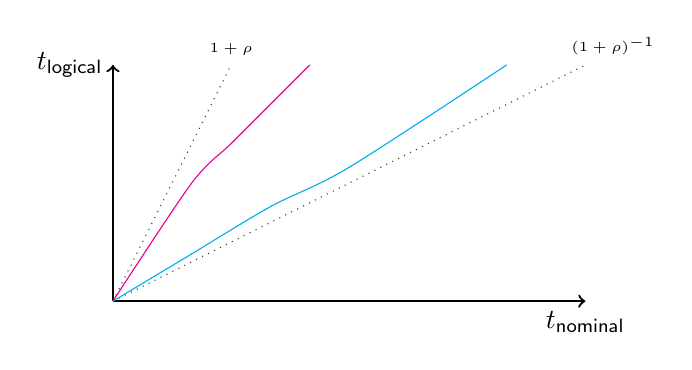
\begin{tikzpicture}
        \draw[->, thick] (0, 0) -- (6, 0) node[below] {$t_{\mathsf{nominal}}$};
        \draw[->, thick] (0, 0) -- (0, 3) node[left] {$t_{\mathsf{logical}}$};

        \draw[dotted, color = darkgray] (0, 0)--(6, 3) node[above, color = black, xshift=1em] {\tiny $(1 + \clockDrift)^{-1}$};
        \draw[dotted, color = darkgray] (0, 0)--(1.5, 3) node[above, color = black] {\tiny $1 + \clockDrift$};

        \draw[opacity=0]  (0,0) -- (1,1) -- (1.5, 2) -- (2, 2.5)  -- (3, 3);

        \draw [magenta] plot [smooth] coordinates { (0,0) (1,1.5) (1.5, 2) (2, 2.5) (2.5, 3)};

        \draw [cyan] plot [smooth] coordinates { (0, 0) (0.5, 0.3) (1, 0.6) (2, 1.2) (3, 1.7) (5, 3)};
    \end{tikzpicture}

    \caption{An illustration of drifting clocks within a $(0.5, 2)$-linear envelope (i.e., $\clockDrift = 1$). Without clock synchronization, two clocks (illustrated in magenta and cyan, respectively) deviate from each other unboundedly.}
    \label{fig:drifting-clocks}
\end{figure}


Note that time in the drifting clock model are real values, while our protocol execution model divides time into discrete integer-numbered steps.
%
In order to ``insert'' real-valued time into this structure, we model drifting local clocks as \funcDriftingClock, derived from the global clock functionality in~\cite{TCC:KMTZ13}.
%
In \funcDriftingClock, nominal time is defined by the number of times that the clock functionality moves forward the time-step variable $\tau$ (which is an internal variable and is unknown to the parties).
%
Instead of directly receiving the time from \funcDriftingClock, parties receive ``ticks'' from \funcDriftingClock which indicates that they should advance their local round number.
%
\funcDriftingClock advances the nominal time when all (honest) participants claim they have finished their computation in the current round.
%
Additionally, \funcDriftingClock allows the adversary to ``push'' or ``stall'' honest clocks, as long as these operations do not violate the \clockDrift-bounded linear envelope assumption.
%
We present \funcDriftingClock in~\cref{functionality:drifting-clock}.

\begin{remark}
    As opposed to the classical distributed computing setting (cf.~\cite{JACM:DwoLynSto88}) where rounds/time steps are defined as intervals of equal length in the view of an external real-time clock, in our model \funcDriftingClock does not guarantee that rounds/time steps are of equal duration.
    %
    In fact, the notions of `time' and `duration' are not defined in the UC setting.
    %
    Yet, our model shows the same effect in restricting local clock counters staying in a bounded linear envelope with respect to the nominal clock counter; moreover, the same amount of computation is carried out per local time counter increment --- which means that in the same window of nominal time, a faster CPU will solve more PoWs than a slower one.
\end{remark}

\begin{cccFunctionality}
    {\funcDriftingClock}
    {drifting-clock}
    {The drifting global clock.}

    This functionality maintains state variables as follows.

    \addtocounter{table}{-1}
    \begin{tabularx}{.9\textwidth}{c X}
        \toprule[.3mm]
        \textbf{State Variable}
         & \textbf{Description}
        \\ \midrule[.3mm]
        $\clockDrift \gets 0$
         & The bound on clock drifts.
        \\ \midrule
        $\partyset \gets \emptyset$
         & The set of registered parties $\party = (\pid, \sid)$.
        \\ \midrule
        $F \gets \emptyset$
         & The set of registered functionalities (together with their session identifier).
        \\ \midrule
        $\tau_\sid \gets 0$
         & The nominal-time variable for session \sid.
        \\ \midrule
        $d_\party \gets 0$
         & The clock-update variable for $\party = (\pid, \sid) \in \partyset$.  $d_\party$ is set to $1$ after \party finishes a round.
        \\ \midrule
        $b_\party \gets 1$
         & The tick-budget variable for $\party = (\pid, \sid) \in \partyset$.
        \\ \midrule
        $d(\F, \sid) \gets 0$
         & The clock-update variable for $(\F, \sid) \in F$.
        \\ \bottomrule[.3mm]
    \end{tabularx}

    \paragraph{Setting the drift:}
    %
    \begin{cccItemize}[nosep]
        \item Upon  receiving $(\textsc{set-drift}, \sid, r)$ from the adversary \adv, \textbf{if} \textsc{set-drift} has never been received then set $\clockDrift = r$. Return $(\textsc{set-drift}, \sid, \ok)$ to \adv.
    \end{cccItemize}

    \paragraph{Clock capabilities:}
    %
    \begin{cccItemize}[nosep]
        \item Upon receiving $(\textsc{clock-update}, \sid_C)$ from some party $\party \in \partyset$ set $d_\party \gets 1$ and $b_\party \gets b_\party - 1$; execute \textit{Time-Update} and forward $(\textsc{clock-update}, \sid_C , \party)$ to \adv.

        \item Upon receiving $(\textsc{clock-update}, \sid_C)$ from some functionality \F in a session \sid such that $(\F, \sid) \in F$ set $d(\F, \sid) \gets 1$, execute \emph{Time-Update} and return $(\textsc{clock-update},\allowbreak \sid_C, \F)$ to this instance of \F.

        \item Upon receiving $(\textsc{clock-forward}, \sid_C , \party)$ from \adv where $\party \in \partyset$, if $d_\party = 0$ or it is about to violate the \clockDrift-bounded linear envelope on \party, ignore the message.
        %
        Otherwise, update $d_\party = 0$ and $b_\party \gets b_\party + 1$; return $(\textsc{clock-forward-ok}, \sid_C , \party)$ to \adv.

        \item Upon receiving $(\textsc{clock-backward}, \sid_C , \party)$ from \adv where $\party \in \partyset$, if $d_\party = 0$ or it is about to violate the \clockDrift-bounded linear envelope on \party, ignore the message.
        %
        Otherwise, update $b_\party \gets b_\party - 1$; return $(\textsc{clock-backward-ok}, \sid_C , \party)$ to \adv.

        \item Upon receiving $(\textsc{clock-tick}, \sid_C)$ from any participant \party --- including the environment on behalf of a party --- or the adversary on behalf of a corrupted party \party (resp. from any ideal---shared or local---functionality \F), execute procedure \textit{Time-Update}, return $(\textsc{clock-tick}, \sid_C, d_{\party})$ (resp. $(\textsc{clock-tick}, \sid_C, d_{(\F, \sid)})$) to the requestor (where \sid is the session id of the calling instance).

        \item Upon receiving $(\textsc{clock-read}, \sid_C)$ from the adversary or the wapper functionalities, return $(\textsc{clock-read},\sid_C, \tau_{\sid})$ to the requestor (where \sid is the session id of the calling instance).
    \end{cccItemize}

    \medskip\emph{Procedure Time-Update:}
    %
    For each session \sid do: If (i) $d_{(\func, \sid)} = 1$ for all $\func \in F$, and (ii) $d_\party = 1$ and $b_\party \le 0$ for all honest parties $\party = (\cdot, \sid) \in \partyset$, then update $\tau_\sid \gets \tau_\sid + 1$, $d_{(\func,\sid)} \gets 0$ and $b_\party \gets b_\party + 1$ for all parties $\party = (\cdot, \sid) \in \partyset$.
    %
    Additionally, for all parties $\party = (\cdot, \sid) \in \partyset$ with $b_\party > 0$, update $d_\party \gets 0$.
\end{cccFunctionality}


We adapt the traditional definition of the clock synchronization problem (cf.~\cite{JCSS:DHS86,JACM:SriTou87}) to our permissionless setting.
%
In~\cref{def:clock-properties}, we consider two properties, \emph{bounded skew} and \emph{accuracy}, that establish upper bounds \maxSkew and $\varGamma$ on honest clock skew and their deviation from the nominal time, respectively.

\begin{definition}
    [Clock Synchronization]
    \label{def:clock-properties}
    There exist constants $\maxSkew \in \mathbb{N}$, $\varGamma \in \mathbb{R}^+$ such that honest parties' logical clocks satisfy the following two properties:
    %
    \begin{cccItemize}[nosep]
        \item \emph{\bf Bounded skew (with parameter $\maxSkew \in \mathbb{N}$).}
        %
        Let $\round_1, \round_2$ be the reported logical clocks of two
        honest parties at any nominal time $r$.
        %
        Then $|\round_ 1 - \round_2| \le \maxSkew$.

        \item \emph{\bf Accuracy (with parameter $\varGamma \in \mathbb{R}^+$).}
        %
        Each honest party's logical clock stays in a $(U, L)$-linear envelope with respect to the nominal time $r$, where $U = 1 + \varGamma$ and $L = 1 / (1 + \varGamma)$.
    \end{cccItemize}
\end{definition}

\subsection{Random Oracle, Network and Adversarial Model}
\label{subsec:ro-network-corruption}

\paragraph{Random oracle.}
%
By convention, we model the cryptographic hash function $H$ with output in $\{0, 1\}^\kappa$ (which is used to generate proofs of work [PoWs]) as a random oracle \funcRO~\cite{CCS:BelRog93}.

\input{functionalities/random-oracle}

We express our honest majority condition in terms of computational power, measured in particular by the number of queries to the RO that the parties are allowed to make per \emph{nominal time-step}, as opposed to expressing it by the number of parties (i.e., the ``flat'' model where parties are assumed to have equal computational power---cf.~\cite{EC:GarKiaLeo15}).

\begin{definition}[Honest Majority]
    Let $h_r, t_r$ denote the number of \emph{alert} and \emph{non-alert} random oracle queries at \emph{nominal} time $r$, respectively.
    %
    Then, for all $r \in \mathbb{N}$, it holds that $h_r > t_r$.
\end{definition}

This restriction on the number of RO queries is captured by a wrapper functionality on \funcRO via counting the number of \emph{alert} and other queries (see below) per nominal-time step.
%
The adversary is allowed to dynamically and adaptively determine the number of alert random oracle queries per nominal-time step, as long as it does not violate the restrictions imposed by the $(\gamma, s)$-respecting environment (see~\cref{def:respecting-environment} in the sequel).

\begin{cccFunctionality}
    {\wrapper{\funcRO}}
    {random-oracle-wrapper}
    {The random oracle wrapper.}

    This functionality maintains state variables as follows.

    \addtocounter{table}{-1}
    \begin{tabularx}{.9\textwidth}{c  X}
        \toprule[.3mm]
        \textbf{State Variable}
         & \textbf{Description}
        \\ \midrule[.3mm]
        $\partyset \gets \emptyset$
         & The set of registered parties; the current set of corrupted parties is denoted by $\partyset'$.
        \\ \midrule
        $\tau \gets 0$
         & The (real-time) clock tick counter.
        \\ \midrule
        $h_\tau$
         & An upper bound which restricts the \func-evaluations of all alert parties at time $\tau$.
        \\ \midrule
        $q_\honestPartySet, q_\adv \gets 0$
         & The alert/adversary evaluation counter.
        \\ \bottomrule[.3mm]
    \end{tabularx}

    \paragraph{Pre-mining attack handling (executed only if $\tau = 0$):}
    %
    \begin{cccItemize}[nosep]
        \item Upon receiving $(\textsc{eval}, \sid, x)$ from \adv on behalf of a corrupted party $P \in \partyset'$, forward the request to \funcRO and return to \adv whatever \funcRO returns.

        \item Upon receiving $(\textsc{Retrieved}, \sid)$ from \funcCRS, set $\tau = 1$.
    \end{cccItemize}

    \paragraph{Relaying inputs to the random oracle:}
    %
    \begin{cccItemize}[nosep]
        \item Upon receiving $(\textsc{eval}, \sid, x)$ from \adv on behalf of a corrupted party $P \in \partyset'$ or a de-synchronized party \party, first execute \textit{Round Reset}, then do the following.
        %
        \begin{cccEnum}[nosep]
            \item Set $q_\adv \gets q_\adv + 1$.
            \item \textbf{If} $q_\adv \le h_\tau$ \textbf{then} forward the request to \funcRO and return to \adv whatever \funcRO returns.
        \end{cccEnum}

        \item Upon receiving $(\textsc{eval}, \sid, x)$ from an alert party \party, first execute \textit{Round Reset}, then do the following.
        %
        \begin{cccEnum}[nosep]
            \item Set $q_\honestPartySet \gets q_\honestPartySet + 1$.
            \item \textbf{If} $q_\honestPartySet \le h_\tau$ \textbf{then} forward the request to \funcRO and return to \party whatever \funcRO returns.
            \item \textbf{If} $q_\honestPartySet \ge h_\tau$ \textbf{then} send $(\textsc{clock-update}, \sid_C)$ to \funcDriftingClock.
        \end{cccEnum}
    \end{cccItemize}

    \paragraph{Corruption handling:}
    %
    \begin{cccItemize}[nosep]
        \item Upon receiving $(\textsc{corrupt}, \sid, \party)$ from the adversary, set $\partyset' \gets \partyset' \cup \party$.
    \end{cccItemize}

    \medskip\emph{Procedure Round-Reset:}
    %
    Send $(\textsc{clock-read}, \sid_C)$ to \funcDriftingClock and receive $(\textsc{clock-read}, \allowbreak \sid_C, \tau')$ from \funcDriftingClock. If $|\tau - \tau' | > 0$, then do the following.
    %[
    \begin{cccEnum}[nosep]
        \item Set $q_\honestPartySet, q_\adv \gets 0$ and $\tau \gets \tau'$.

        \item Send $(\textsc{next-round})$ to \adv and receive as response $(\textsc{next-round}, h^*_{\tau'})$.
        %
        \textbf{If} $(h_1, h_2, \ldots, h'_{\tau'})$ is $(\gamma, s)$-respecting (\cref{def:respecting-environment}) \textbf{then} set $h_{\tau'} = h'_{\tau'}$; \textbf{else} set $h_{\tau'} = h_{\tau' - 1}$.
    \end{cccEnum}
\end{cccFunctionality}


In addition, pre-mining attack prevention is captured by restricting the number of adversarial queries after a fresh CRS is released (which we model as \funcCRS).

\begin{cccFunctionality}
    {\funcCRS}
    {CRS}
    {The common reference string.}

    The functionality is parameterized by a distribution $\mathcal{D}$.

    \begin{cccItemize}[noitemsep]
        \item \textbf{Retrieve.} Upon receiving $(\textsc{Retrieve}, \sid)$ from some party \party (or from \adv on behalf of a corrupted \party), do the following:
        %
        \begin{cccEnum}[nosep]
            \item If activated for the first time, choose a value $d \gets \mathcal{D}$, and send $(\textsc{Retrieved}, \sid)$ to \wrapper{\funcRO} and \wrapper{\funcDiffuse}.

            \item Return $(\textsc{Retrieve}, d)$ to \party.
        \end{cccEnum}
    \end{cccItemize}
\end{cccFunctionality}

\paragraph{The bounded-delay network.}
%
Regarding communication amongst parties, we consider a peer-to-peer diffusion network, where the message dissemination has an (unknown) \delay-bounded delay.
%
In more detail, an honest message sent at time $t$ will be received by all other honest parties before time $t + \delay$; regarding messages sent by the adversary, if $t$ is the earliest time such that at least one honest party receives those messages, they are guaranteed to be delivered to all honest parties before time $t + \delay$ (i.e., honest parties keep ``echoing'' messages).

We capture this communication network with \funcDiffuse (\cref{functionality:diffuse}).
%
Recall that existing diffuse functionalities (cf.~\cite{C:BMTZ17}) model delays in the following manner:
%
There is a fetch counter per message per recipient such that when each time an honest party \party is activated and received a new tick from the clock, \party fetches on \funcDiffuse which reduces counters by $1$ for all messages delivering to \party; she then receives a subset of those messages with counters reset to $0$.
%
Regarding the adversary, he can increase the counter for each message and recipient for up to \delay in accumulation (as well as swapping the order of messages).

By convention, different types of messages are diffused by different functionalities, and we write $\funcDiffuse^{\textsf{bc}}$, $\funcDiffuse^{\textsf{input}}$, $\funcDiffuse^{\textsf{tx}}$ to denote the network for chains, input blocks and transactions.

\input{functionalities/diffuse}

We highlight that such mechanism does \emph{not} work in our drifting clock model with \funcDriftingClock (it only works with a global clock where parties proceed with the same speed).
%
This is because, when modeling delays via fetches on the diffuse functionality, honest parties that experience relatively fast local rounds would request more \textsc{fetch} commands than the slow ones in the same window of nominal time --- i.e., if an honestly-sent message is set the same delay for two parties then it delivers to the fast one earlier; yet our goal is to model delays measured in the perspective of the nominal time (regardless of parties' local understanding of time).

We resolve this issue by introducing a new wrapper on \funcDiffuse (\cref{functionality:wrapper-diffuse}) that restricts the adversary's capability to delay messages for up to \delay nominal time.
%
After registering on \funcDriftingClock to learn the nominal time ticks, the wrapper functionality dynamically relays parties' \textsc{fetch} request to \funcDiffuse so that in every nominal-time step, exactly one fetch operation is relayed to \funcDiffuse for each honest party (even if that honest party receives multiple ticks from \funcDriftingClock).
%
Meanwhile, for each party \party that proceeds slowly and may not activate in a given nominal time, the wrapper queries \funcDiffuse on behalf of \party, buffers the response messages and delivers them to \party upon the next time \party interacts with the wrapper.

\begin{cccFunctionality}
    {\wrapper{\funcDiffuse}}
    {wrapper-diffuse}
    {The wrapper of diffuse network.}

    This functionality maintains state variables as follows.

    \addtocounter{table}{-1}
    \begin{tabularx}{.9\textwidth}{c  X}
        \toprule[.3mm]
        \textbf{State Variable}
         & \textbf{Description}
        \\ \midrule[.3mm]
        $\partyset \gets \emptyset$
         & The set of registered parties; the current set of corrupted parties is denoted by $\partyset'$.
        \\ \midrule
        $\tau \gets 0$
         & The (real-time) clock tick counter.
        \\ \midrule
        $\mathsf{fetch}(\party, \tau) \gets 0$
         & The fetch variable for party \party at nominal time $\tau$.
        \\ \midrule
        $\mathsf{buffer}_\party \gets []$
         & The fetch buffer for party \party.
        \\ \bottomrule[.3mm]
    \end{tabularx}

    \paragraph{Relaying inputs to the diffuse network:}
    %
    \begin{cccItemize}[nosep]
        \item Upon receiving $(\textsc{diffuse}, \sid, m)$ from \adv on behalf of some corrupted $\party \in \partyset'$, parse $m$ as blocks $\block_1, \ldots, \block_n$.
        %
        For each $\block_i$, if $\block_i$ has not been queried to \funcRO, send $(\textsc{eval}, \sid, \block_i)$ from a corrupted party.

        \item Upon receiving $(\textsc{fetch}, \sid)$ from an honest party \party, if $\mathsf{fetch}(\party, \tau) = 1$ ignore this request.
        %
        Otherwise, execute the following:
        %
        \begin{cccEnum}[nosep]
            \item Forward $(\textsc{fetch}, \sid)$ to \funcDiffuse and recevie as response $\vec{M}$, return $\mathsf{buffer}_\party \concat \vec{M}$.
            \item Set $\mathsf{buffer}_\party \gets []$ and $\mathsf{fetch}(\party, \tau) \gets 1$.
        \end{cccEnum}
    \end{cccItemize}

    \paragraph{Corruption handling:}
    %
    \begin{cccItemize}[nosep]
        \item Upon receiving $(\textsc{corrupt}, \sid, \party)$ from the adversary, set $\partyset' \gets \partyset' \cup \party$.
    \end{cccItemize}

    \medskip\emph{Procedure Round-Reset:}
    %
    Send $(\textsc{clock-read}, \sid_C)$ to \funcDriftingClock and receive $(\textsc{clock-read}, \allowbreak \sid_C, \tau')$ from \funcDriftingClock. If $|\tau - \tau' | > 0$, then do the following.
    %[
    \begin{cccEnum}[nosep]
        \item Set $\tau \gets \tau'$.

        \item  For each honest party $\party$ such that $\mathsf{fetch}(\party, \tau) = 0$, send $(\textsc{fetch}, \sid)$ to \funcDiffuse from \party and recevie as response $\vec{M}$, set $\mathsf{buffer}_\party \gets \mathsf{buffer}_\party \concat \vec{M}$.
        %
        For each honest party $\party$ such that $\mathsf{fetch}(\party, \tau) = 1$, set $\mathsf{fetch}(\party, \tau) \gets 0$.

        \item Send $(\textsc{clock-update}, \sid_C)$ to \funcDriftingClock.
    \end{cccEnum}
\end{cccFunctionality}


\paragraph{Dynamic availability and respecting environment.}
%
In order to apply a more fine-grained classification on protocol participants, we follow the treatment in~\cite{CCS:BGKRZ18} and classify parties into different types based on their accessible resources and synchronization states.
%
Specifically, a party is (i) \emph{operational} if she is registered with the random oracle \funcRO, and \emph{stalled} otherwise; (ii) \emph{online} if she is registered with the network \funcDiffuse, and \emph{offline} otherwise; (iii) \emph{time-aware} if she is registered with the drifting clock \funcDriftingClock, and \emph{time-unaware} otherwise; and (iv) \emph{synchronized} if she has been participated in the protocol for sufficiently long time and held ``synchronized state'' and ``synchronized time'' with other synchronized parties, and \emph{desynchronized} otherwise.

We define \emph{alert} parties based on the classification above.
%
Specifically, alert parties are those who have access to all the resources and are synchronized.
%
They are the core set of parties to carry out the protocol.

Next, we define a ``respecting environment'' in terms of the computational power (cf.~\cite{TCC:GarKiaShe22}) as opposed to number of parties (cf.~\cite{C:GarKiaLeo17,EPRINT:GarKiaLeo20}).
%
Our honest-majority assumption is that during the whole protocol execution, the alert computational power is higher than the adversarial one.
%
We restrict the environment so that the number of such queries will be bounded in a certain fashion.

\begin{definition} \label{def:respecting-environment}
    For $\gamma \in \mathbb{R}^+$ we call the sequence $(h_r)_{r \in [0, B)}$, where $B \in \mathbb{N}$, $(\gamma, s)$-respecting if for any set $S \subseteq [0, B)$ of at most $s$ consecutive integers, $\max_{r \in S} h_r \le \gamma \cdot \min_{r \in S} h_r$.
\end{definition}

\subsection{Blockchain Notation}

A block with target $T \in \mathbb{N}$ is a quadruple of the form $\block = \langle ctr, r, h, x \rangle$ where $ctr, r \in \mathbb{N}$, $h \in \{0, 1\}^{\kappa}$ and $x \in \{0, 1\}^*$.
%
A blockchain \chain is a (possibly empty) sequence of blocks; the rightmost block is denoted by \chainHead{\chain} (note $\chainHead{\varepsilon} = \varepsilon$).
%
These blocks are chained in the sense that if $\block_{i + 1} = \langle ctr, r, h, x \rangle$, then $h = H(\block_i)$.
%
We use \timestamp{\block} to denote the \emph{timestamp} of \block.
%
We denote by \chainPrefixUB{\chain}{t} the chain resulting from ``pruning'' the least number of rightmost blocks so that all block timestamps are less than $t$.
%
Let $\parallelChains = \langle \chain_1, \chain_2, \ldots, \chain_m \rangle$ denote $m$ \emph{parallel} chains and $\parallelChains_j$ the $j$-th chain $\chain_j$ in \parallelChains.

Next, we introduce some basic string notation, which will be useful when describing our multi-chain-oriented PoW mechanism.
%
For a $\kappa$-bit string $s$, where $\kappa$ is the security parameter, we will use $s_i~(i \in [m])$ to denote the $i$-th bit of $s$, \stringSegment{s}{i}{m} to denote the $i$-th segment after $s$ is equally divided into $m$ segments---i.e., $\stringSegment{s}{i}{m} = s_{[(i - 1) * \kappa / m ]+ 1}, \ldots, s_{i * \kappa / m}$.
%
Further, we will write \stringRev{s} as the reverse of string $s$ (i.e., the string obtained by reversing the order of its bits), and use \stringSegmentRev{s}{i}{m} to denote the reverse of the $i$-th segment.

Finally, we introduce some array operations, following the notation in~\cite{JACM:DLPSW86}, that will be useful when describing the protocol.
%
Let $\mathbf{V} = (v_1, \ldots, v_n)$ be a real array of $n$ elements and denote $\tilde{\mathbf{V}} = (\tilde{v}_1, \ldots, \tilde{v}_n)$ the array after ordering $\mathbf{V}$ non-decreasingly.
%
We define the operations \textsf{reduce} and \textsf{select}.
%
Intuitively, \textsf{reduce} with parameter $\mathbf{V}$ and $\eta$ first orders $\mathbf{V}$ non-decreasingly and then ``trims'' the $\eta$ largest and $\eta$ smallest elements in $\tilde{\mathbf{V}}$; \textsf{select} with parameter $\mathbf{V}$ and $\eta$ first orders $\mathbf{V}$ non-decreasingly and then selects every first element of $\eta$ consecutive elements and forms them as a new array.
%
Formally,
%
\begin{equation} \label{eq:reduce-select}
    \mathsf{reduce}(\mathbf{V}, \eta) = (\tilde{v}_{\eta + 1}, \ldots, \tilde{v}_{n - \eta})
    ~~\text{and}~~
    \mathsf{select}(\mathbf{V}, \eta) = (\tilde{v}_1, \tilde{v}_{\eta + 1}, \tilde{v}_{2\eta + 1}, \ldots).
\end{equation}
%
Additionally, for an array $\mathbf{V}$, let $\mathsf{avg}(\mathbf{V})$ denote the average of its elements, and $\med(\mathbf{V})$ denote the median.

\subsection{Weak/Approximate Agreement}
\label{subsec:weak-approximate-agreement}

\paragraph{Weak agreement.}
%
A variant of Byzantine agreement --- \emph{Weak Agreement} -- relaxes the agreement property to allow some parties to output a special failing symbol $\bot$ while requiring all non-$\bot$ outputs being consistent \cite{JoA:Dolev82}.
%
This simple primitive has been widely used in building stronger notion of agreement (e.g., graded agreement).
%
We here provide the definition of Weak Agreement.

\begin{definition}
    [Weak Agreement]
    \label{def:weak-agreement}
    A protocol $\Pi$ implements Weak Agreement provided it satisfies the following two properties:
    %
    \begin{cccItemize}[nosep]
        \item \emph{\textbf{Weak Agreement}}: There exists $y \in \{0, 1\}$ such that all honest parties output $y_i \in \{ y, \bot \}$.

        \item \emph{\textbf{Validity}}: If all honest parties have the same input $b \in \{0, 1\}$, they all output $y_i = b$.
    \end{cccItemize}
\end{definition}

\paragraph{Approximate agreement.}
%
\emph{Approximate Agreement} (AA), formulated in~\cite{JACM:DLPSW86}, is a variant of the Byzantine agreement problem~\cite{JACM:PeaShoLam80,TOPLAS:LamShoPea82} in which processes start with arbitrary real values rather than Boolean values or values from some bounded range, and in which approximate, rather than exact, agreement is the desired goal.
%
In the classical distributed computing literature, AA has served as a fundamental building block to achieve clock synchronization (see, e.g.,~\cite{PODC:LunLyn84,PODC:MahSch85,PODC:LenLos22}).

Next, we present a definition of AA which captures adaptive security.
%
Conventionally, the goal is to let honest parties agree on outputs where the difference between any two of them is upper-bounded by a constant.
%
In this paper, we provide an alternate yet equivalent definition which asks for a ``concentration'' on the outputs compared with the inputs.
%
We denote $\epsilon$ as the ``quality'' of the agreement---i.e., the ratio between honest-input distance and output distance.

\begin{definition}
    [Approximate Agreement]
    \label{def:approximate-agreement}
    A protocol $\Pi$ is an $\epsilon$-secure protocol for Approximate Agreement provided it satisfies the following two properties:
    %
    \begin{cccItemize}[nosep]
        \item \emph{\textbf{$\epsilon$-Agreement}}: There is a round after which (i) any two honest parties hold inputs with difference at most $\ell$, and (ii) any two honest parties return outputs with difference at most $\epsilon \cdot \ell$ (where $0 < \epsilon < 1$) if queried by the environment.

        \item \emph{\textbf{Validity}}: The output returned by an honest party \party falls in the convex hull of the inputs of all parties at round $1$ that are honest at the round \party's output is produced.
    \end{cccItemize}
\end{definition}


\section{Permissionless Weak/Approximate Agreement}
\label{sec:reaching-weak-approx-agreement}

In this section we consider weaker forms of agreement --- namely, weak agreement and approximate agreement as introduced in~\cref{subsec:weak-approximate-agreement} --- in the permissionless setting, and show that, when appropriately parameterized, they can be achieved in constant time against a minority of corrupted computational power.
%
We present two protocols: first, a protocol that is simple and easy to understand, but which tolerates only one-third of corrupted computational power.
%
We then improve this protocol to tolerate a dishonest minority and, in the context of AA, achieve better output quality (recall~\cref{def:approximate-agreement}).\footnote{Translating protocols presented in this section to the PoS setting (with dynamic availability) is straightforward, as the core mechanism that we use---\mforone PoW---can be emulated by independently evaluating multiple different VRF outputs.}

For simplicity, we consider a single protocol invocation and present our protocols in the \emph{static} setting where parties are always online and their number is fixed yet unknown to the protocol participants, and we assume a global clock and a diffusion network with \delay-bounded delay.
%
Later, in~\cref{sec:permissionless-smr}, we use the weak/approximate agreement protocols as sub-routines in a dynamic environment with drifting clocks.

\subsection{Weak/Approximate Agreement against a $(1/3)$-Bounded Adversary}
\label{subsec:apa-one-third}

We first provide a simple protocol that solves Weak/Approximate Agreement against an adversary that controls up to one-third of the computational power.
%
At a high level, in this protocol parties first use \mforone PoW to mine and exchange messages containing their input value (concatenated with a random string for uniqueness) for a pre-determined number of $\ell$ rounds; then each party \party decides its output locally based on the messages that it has received.

The protocol is parameterized by $\ell$ (the termination time), $m$ (the number of parallel mining procedures) and $T$ (a pre-determined PoW target value).
%
A party \party starting with input $v$ queries the RO and gets $u = H(r \concat v)$ where $r$ is a $\kappa$-bit random string.
%
For every ``chunk'' \stringSegment{u}{i}{m} of $\kappa / m$ bits, \party checks if $\stringSegment{u}{i}{m} < T$.
%
If \party solves a PoW in any of the chunks, it diffuses $(r, v)$ to the network.
%
Note that $(r, v)$ will be counted independently for different succeeding chunks; e.g., if a valid PoW is found in $m / 2$ segments, $(r, v)$ will be counted for $m / 2$ times.
%
Parties keep listening to the network and book-keep all valid PoW messages, extracting their corresponding values in an array \textbf{V}.

Parties decide their output based on their local array \textbf{V} at the end of round $\ell$.
%
For Weak Agreement, they output $0$ ($1$ resp.) iff. more than two-thirds of the elements in \textbf{V} are $0$s ($1$s resp.); and $\bot$ otherwise.
%
Regarding Approximate Agreement, the output decision procedure then follows the approach in~\cite{JACM:DLPSW86}:
%
For an ordered array \textbf{V} of size $n$, the smallest and largest $n / 3$ values are dropped and the party outputs the midpoint of the remaining values (i.e., the average of the maximum and minimum element).

The full description of the protocol is presented in~\cref{protocol:one-third-approximate-consensus}.

\begin{cccProtocol}
    {$\mathsf{{\frac{1}{3}-}ApproxAgr}(\ell, m, T)$}
    {one-third-approximate-consensus}
    {Weak/Approxmate Agreeement tolerating a $(1 / 3)$-bounded adversary.}

    \begin{algorithmic}[1]
        \LineComment{The following code is executed in each round \round (\val is the party input)}
        \If{$\round \le \ell$} \Comment{Step 1: mine and exchange messages.}

        \State{Fetch information and denote incoming PoW messages by $((r_1, v_1), \ldots, (r_n, v_n))$}
        \For{each $(r_i, v_i)$}
        \State{Set $c = |\{j \mathbin| j \in [m] \wedge \stringSegment{H(r_i, v_i)}{j}{m} < T\}|$}
        \State{Append $v_i$ to $\mathbf{V}$ for $c$ times}
        \EndFor

        \State{Set $u \gets H(ctr, \val)$}
        \oneLineIf{$\exists j \in [m]$ s.t. $\stringSegment{u}{j}{m} < T$}{Diffuse $(ctr, \val)$}

        \State{$ctr \gets ctr + 1$}

        \Else  \Comment{Step 2: decide output.}

        \State{Order $\mathbf{V}$ non-decreasingly and denote $n \gets |\mathbf{V}|$} \label{code:ordered-array}

        \If{deciding output for weak agreement}
        \oneLineIf{$\mathbf{V}_{n / 3} = \mathbf{V}_{2n / 3}$}{output $\mathbf{V}_{n / 3}$ \textbf{else} output $\bot$}
        \ElsIf{deciding output for approximate agreement}
        \State{Output the mid point of $\mathsf{reduce}(\mathbf{V}, n / 3)$}
        \EndIf

        \EndIf
    \end{algorithmic}
\end{cccProtocol}

Note that different parties may work on different sets of messages when the adversary chooses to hold and deliver its own PoW message at the last round (so that honest parties have no time to diffuse this message to others).
%
Nonetheless, for sufficiently large $\kappa$ and suitable value of $\ell$, the messages generated by different parties are roughly proportional to their computational power.
%
Thus, for all arrays held by honest parties, they will share a large (yet unknown) common subset.

\begin{lemma} \label{lemma:one-third-apa}
    Let \delay denote the upper bound on network delay, $h$ and $t$ denote the number of honest and adversarial queries per round ($h > 2t$), and $m$ be the number of independent PoW mining.
    %
    Let $V$ denote the honest input set ($V = \{0, 1\}$ for Weak Agreement and $V \subseteq \mathbb{R}$ for Approximate Agreement) and $\mathbf{V}$ denote the ordered array of PoW messages received by party \party after round $\ell$ (line~\ref*{code:ordered-array} in~\cref{protocol:one-third-approximate-consensus}), and assume that $\ell > 4 \delay$ and $m = \bigTheta(\log^2 \kappa)$.
    %
    Then, for any two honest parties $\party, \party'$ (possibly $\party = \party'$) and $\mathbf{V}, \mathbf{V}'$ with size $n, n'$, respectively, it holds that
    %
    \[ \min V \le \mathbf{V}_{n / 3} \le \mathbf{V}'_{2n' / 3} \le \max V, \]
    %
    except with probability negligible in $\kappa$.
\end{lemma}

\begin{proof}
    Let $\mathbf{V}^h \subseteq \mathbf{V}$ denote the subset of messages generated by the honest parties before round $\ell - \delay$.
    %
    Let $\mathcal{H}$ denote the set of honest parties at the end of round $\ell$, and suppose it holds that
    %
    \begin{equation} \label{eq:one-third-aa}
        \forall \party_j \in \mathcal{H}, \Big| \bigcap_{\party_i \in \mathcal{H}} \mathbf{V}^h_i \Big| \ge 2 |\mathbf{V}_j| / 3,
    \end{equation}
    %
    then for $\mathbf{V}$ held by any honest party, it would hold that $\min V \le \mathbf{V}_{n / 3} \le \med(\bigcap_{\party_i \in \mathcal{H}} \mathbf{V}^h_i) \le \mathbf{V}_{2n / 3} \le \max V$, which would conclude the proof.

    Now we only need to verify \cref{eq:one-third-aa}.
    %
    Let $X$ denote the number of PoW messages honest parties generated in the first $(\ell - \delay)$ rounds, and $Y$ denote the number of successful PoWs the adversary generated in the first $\ell$ rounds, plus all the honest PoWs in the last \delay rounds.
    %
    Since $\ell > 4 \delay$, we have $\EX[X] > \EX[2Y]$.
    %
    Note that $\EX[X] = \bigTheta(\EX[2Y]) = \bigTheta(\log^2 \kappa)$.
    %
    Now, by letting $\epsilon \in (0, (\EX[X] / \EX[2Y] - 1) / 2 )$ be a constant and applying the Chernoff bound (\cref{thm:chernoff-bounds}), we get
    %
    \[ \Pr[X > 2Y] \ge \Pr[X > (1 - \epsilon) \EX[X]] \wedge \Pr[2Y < (1 + \epsilon) \EX[2Y]] \ge 1 - \exp(-\bigOmega(\log^2 \kappa)), \]
    %
    which happens with overwhelming probability in $\kappa$, the security parameter.
\end{proof}

Given the good properties satisfied by $\mathbf{V}$ as described in~\cref{lemma:one-third-apa}, we conclude that (i) by comparing $\mathbf{V}_{n / 3}$ and $\mathbf{V}_{2n / 3}$, honest parties reach Weak Agreement; and (ii) by applying the mid-point on \textsf{reduce}, honest parties reach Approximate Agreement with concentration quality $1/2$.
%
We prove this for Approximate Agreement in~\cref{thm:apprx-agr-one-third} (and Weak Agreement can be argued alike).

\begin{theorem} \label{thm:apprx-agr-one-third}
    Under the same assumption as in~\cref{lemma:one-third-apa}, \cref{protocol:one-third-approximate-consensus} is a $(1/2)$-secure Approximate Agreement protocol against an adversary that controls less than one-third of the computational power, except with negligible probability in the security parameter.
\end{theorem}

\begin{proof}
    Validity follows directly, since for any honest party $\party_i$, all values in $\mathsf{reduce}(\mathbf{V}_i, |\mathbf{V}_i| / 3)$ are within the convex hull of the honest inputs, and so is the midpoint.

    Regarding $(1/2)$-Agreement, note that there exist a value $u$ such that for any honest party \party and $\mathbf{V}$,  $\mathbf{V}_{n / 3} \le u \le \mathbf{V}_{2n / 3}$ (cf.~\cref{lemma:one-third-apa}).
    %
    For any two honest parties \party and $\party'$ and their respective outputs $v, v'$, let $v_1, v_2$ ($v'_1, v'_2$, resp.) denote the smallest and largest values in $\mathsf{reduce}(\mathbf{V}_i, |\mathbf{V}_i| / 3)$ ($\mathsf{reduce}(\mathbf{V}'_i, |\mathbf{V}'_i| / 3)$, resp.).
    %
    We have
    %
    \[ |v - v'| = (|v_1 - v'_1|  + |v_2 - v'_2|)/ 2 \le (\max V - u + u - \min V|) / 2 = (\max V - \min V) / 2, \]
    %
    which concludes the proof.
\end{proof}

\begin{remark}
    We note that the output quality of a single invocation of AA as \cref{protocol:one-third-approximate-consensus} can be improved when the adversary controls less computational power.
    %
    This is in line with the classical AA algorithm by Dolev \textit{et al.} \cite{JACM:DLPSW86}.
\end{remark}

The output quality $\epsilon$ can be improved by calling the same Approximate Agreement protocol sequentially, with each invocation using the output of the previous one as input, resulting in $n$ sequential calls improving the output quality to $\epsilon' = \epsilon^n$.
%
In the classical setting(s) (point-to-point channels, or PKI), since deterministic termination is guaranteed, the sequential composition of AA protocols is trivial.
%
In a permissionless environment, however, where only a public setup is available, the sequential composition becomes more challenging in that a common reference string is needed for \emph{every} invocation in order to avoid pre-mining.
%
This problem has been addressed in~\cite{EC:GarKiaShe24} for the case of synchronous protocols (i.e., no [unknown] bounded delay) with static number of participants.
%
In~\cref{sec:permissionless-smr}, we show how this mechanism can be adapted to the drifting clock model with fluctuating number of parties.

\subsection{Weak/Approximate Agreement with Optimal Corruption Threshold}
\label{subsec:apa-honst-majority}

\cref{protocol:one-third-approximate-consensus} works only when the adversarial computational power is bounded by one-third, and in terms of AA the protocol offers concentration quality $\epsilon = 1 / 2$.
%
In this section we present a new protocol that improves the corruption threshold to honest majority for both Weak and Approximate Agreement.
%
Moreover, for Approximate Agreement, it achieves $\epsilon$-Agreement for an arbitrarily small $\epsilon > 0$ after a single invocation.

We first provide some intuition on why~\cref{protocol:one-third-approximate-consensus} fails in an honest majority setting, taking Approximate Agreement as an example.
%
Notice that with stronger adversarial computational power, the intersection of PoW message arrays held by an honest party at the decision phase becomes too small to account for two-thirds of its PoW message array.
%
Thus, since the common subset is not large enough, the \textsf{reduce} and mid-point computations can no longer guarantee $\epsilon$-Agreement for $\epsilon = 1 / 2$ and Validity at the same time.
%
In more detail, when the adversarial messages (and inconsistent honest messages due to network delay) can account for more than one-third of the messages, parties need to trim more values from both sides of the ordered array; otherwise, Validity would not hold because the mid-point computation may take some adversarially proposed values as input.
%
However, trimming more than one-third of the elements from both sides hurts $\epsilon$-Agreement, as the inequalities in~\cref{lemma:one-third-apa} no longer stand.

To circumvent the above situation, our solution is to categorize the different PoW messages based on their indices (in the $m$ parallel procedures) where they succeed, and select one message in each procedure to form a message array \textbf{V} of fixed size of $m$ values, thus providing a more refined approach to decide on an output value.

\paragraph{Protocol description.}
%
Here we show how to extend \cref{protocol:one-third-approximate-consensus} to the honest majority setting.
%
The protocol takes two additional parameters $k$ and $\eta$, which are explained below, and runs $m$ PoW-based Byzantine agreement (BA) procedures in parallel (cf.~\cite{EC:GarKiaLeo15})\footnote{We note that, while running a single invocation of such BA procedure \cite{EC:GarKiaLeo15} for $\bigTheta(\log^2 \kappa)$ rounds yields a full agreement, terminating after constantly many rounds does not give any form of weak agreement with overwhelming probability.}.
%
In each procedure, it builds a PoW-based blockchain (which at a high level follows the Nakamoto protocol) and binds the mining procedure of the chain with ``input-blocks'' using \twoforone PoWs (thus, each party maintains $m$ parallel blockchains which we denote by \parallelChains).
%
Specifically, for a RO query output $u$ and each chain index $i \in [m]$, alongside with checking if a block that is used to extend the chain is produced by evaluating $\stringSegment{u}{i}{m} < T$, the \twoforone mining further evaluates the reverse of this chunk \stringSegmentRev{u}{i}{m}.
%
If $\stringSegmentRev{u}{i}{m} < T$, an input-block \inputBlock containing the miner's input is mined and \inputBlock can be included in the corresponding $i$-th blockchain.
%
Yet, a single RO query can produce different valid blocks to extend different blockchains, as well as an input block that can be valid on multiple chains.
%
Refer to~\cref{protocol:approximate-consensus} Line~\ref*{code:mforone-pow-mining-begin} to \ref*{code:mforone-pow-mining-end} to see how the \mforone and \twoforone mining procedures are bound together in order to get $m$ independent parallel instances of the PoW-based BA protocol.
%
Also note that, parties extend each blockchain \chain independent following the longest chain selection rule (as specified in the Bitcoin backbone protocol~\cite{EC:GarKiaLeo15} which we omit the details on chain validation and selection here), and keeps including valid and unique input-blocks with respect to \chain.

After $\ell$ rounds, for each parallel chain $\chain_i$, parties extract all input-blocks in its prefix by pruning blocks based on their timestamp, subject to the ``common prefix'' parameter $k$.\footnote{In ordinary blockchains, after pruning $k$ blocks, parties hold a chain that is a prefix of any other party's with overwhelming probability, hence the term ``common prefix.'' However, since our protocol terminates in constant time, this pruning operation will lead to a common prefix only with constant probability.}
%
Then, these input-blocks are ordered based on their value contained and the median one is picked as the output of chain $\chain_i$.
%
This forms an array $\mathbf{V}$ of size $m$.
%
For Approximate Agreement, each party then decides its output based on its local $\mathbf{V}$ and a parameter $\eta < m / 2$, by first ordering $\mathbf{V}$ and removing the smallest and largest $\eta$ values, selecting the first element of every $\eta$ elements, and computing the average of the selected ones.
%
I.e., they output $\textsf{avg}(\mathsf{select}(\mathsf{reduce}(\mathsf{V}, \eta), \eta))$ and terminate.
%
In terms of Weak Agreement, parties output a value that accounts for a super-majority of the chains if it exists, and $\mathcal{\bot}$ otherwise.

\begin{cccProtocol}
    {$\mathsf{{\frac{1}{2}-}ApproxAgr}(\ell, m, T, k, \eta)$}
    {approximate-consensus}
    {Honest-majority Weak/Approxmate Agreeement.}

    \begin{algorithmic}[1]
        \LineComment{The following code is executed in each round \round (\val is the party input)}

        \If{$r \le \ell$}
        \State{Fetch incoming chains $(\chain_1, \ldots, \chain_N)$}

        \State{$\parallelChainsLocal \gets \mathsf{UpdateLocalChain}(\parallelChainsLocal, \chain_1, \ldots, \chain_N)$}
        \Comment{Select longest valid chains for each index}

        \State{Fetch incoming input-blocks $(\inputBlock_1, \ldots, \inputBlock_k)$}
        \State{Add valid $\inputBlock_1, \ldots, \inputBlock_{k'}$ to \buffer}

        \LineComment{\mforone PoW mining}

        \State{$h \gets \varepsilon$, $st \gets \varepsilon$} \label{code:mforone-pow-mining-begin}
        \For{$i = 1$ \textbf{to} $m$}
        \State{$h \gets h \concat \stringSegment{H(\chainHead{\parallelChains_i})}{i}{m}$}
        \State{Let $\buffer_i$ denote all \inputBlock that are valid yet not included w.r.t. $\parallelChains_i$}

        \State{$st \gets st \concat \blockify(\buffer_i)$\footnote{\blockify translates a sequence of transactions to the ledger state (cf.~\cite{C:BMTZ17}).}}

        \EndFor
        \State{$u \gets H(ctr, r, h, st, val)$}

        \For{$i = 1$ \textbf{to} $m$}
        \Comment{Check if PoW succeeds on any type of block.}
        \oneLineIf{$\stringSegment{u}{i}{m} < T$}{set $\parallelChains_i \gets \parallelChains_i \concat  \langle ctr, r, h, st, val \rangle$ and diffuse $\parallelChains_i$} \Comment{Extend chain}
        \oneLineIf{$\stringSegmentRev{u}{i}{m} < T$}{diffuse  $\inputBlock = \langle ctr, r, h, st, val \rangle$}
        \EndFor
        \State{$ctr \gets ctr + 1$} \label{code:mforone-pow-mining-end}

        \Else

        \State{Initialize $\mathbf{V}$ to an empty array}

        \For{$i$ \textbf{from} $1$ \textbf{to} $m$}
        \Comment{Extract output from parallel chains}

        \State{Initialize $\mathbf{M}$ to an empty array}
        \For{$\inputBlock \in \block \in \chainPrefixUB{\parallelChains_i}{\ell - k}$}
        \State{Parse \inputBlock as $\langle \cdot, \cdot, \cdot, \cdot, val \rangle$ and add $val$ to $\mathbf{M}$}
        \EndFor
        \State{Sort $\mathbf{M}$ and add $\med (\mathbf{M})$ to $\mathbf{V}$}
        \EndFor

        \LineComment{Decide final output}
        \If{deciding output for weak agreement}
        \State{Order $\mathbf{V}$ non-decreasingly and denote $n \gets |\mathbf{V}|$}
        \oneLineIf{$\mathbf{V}_\eta = \mathbf{V}_{n - \eta}$}{output $\mathbf{V}_{\eta}$ \textbf{else} output $\bot$}
        \ElsIf{deciding output for approximate agreement}
        \State{Output $\textsf{avg}(\mathsf{select}(\mathsf{reduce}(\mathbf{V}, \eta), \eta))$}
        \EndIf
        \EndIf
    \end{algorithmic}
\end{cccProtocol}


Next, in the following lemma we show that running the $m$ parallel chains and terminating in a constant number of rounds in a bounded delay network yields good properties on a fraction of the chains.
%
The two properties in~\cref{lemma:apa} have been proven for a synchronous network in~\cite{EC:GarKiaShe24}.
%
Here we extend this result to the bounded-delay network setting.

\begin{lemma} \label{lemma:apa}
    There exist parameterizations of~\cref{protocol:approximate-consensus} such that the following holds.
    %
    Let \parallelChains and $\parallelChains'$ denote the parallel chains held by two honest parties \party and $\party'$ at the end of round $\ell$, respectively.
    %
    There exists a subset $S \subseteq \{1, 2, \ldots, m \}$, $|S| > m - \eta$, such that for all $i \in S$, the following properties hold on chains $\chain = \parallelChains_i$ and $\chain' = \parallelChains'_i$:
    %
    \begin{cccItemize}[nosep]
        \item \emph{\bf Agreement}: $\chainPrefixUB{\chain}{\ell - k} = \chainPrefixUB{\chain'}{\ell - k}$.

        \item \emph{\bf Honest input-block majority}: More than half of the input-blocks included in $\chainPrefixUB{\chain}{\ell - k}$ and $\chainPrefixUB{\chain'}{\ell - k}$ are produced by honest parties.
    \end{cccItemize}
\end{lemma}

\begin{proof}[Proof (sketch)]
    Consider the $i$-th single chain $\chain = \parallelChains_i$ of a party \party.
    %
    There exist parameterizations such that at the end of round $\ell$, with constant probability $p > (m - \eta) / m$, $\chainPrefixUB{\chain}{\ell - k}$ yields a common view with any other honest party and includes a majority of honest input blocks.
    %
    Proving the above claim is mainly a reminiscence of the proof of~\cite[Theorem 2]{EC:GarKiaShe24}, with additionally extending it to the bounded-delay network (see, e.g., \cite[Section 7]{EPRINT:GarKiaLeo14}, for more details).

    Since any two single chains are mutually independent from each other, the probability that these two % good 
    properties hold on more than $p \cdot m  > m - \eta$ chains can be computed by the Chernoff bound (\cref{thm:chernoff-bounds}), with error probability negligibly small in the security parameter $\kappa$ (recall that $m = \polylog \kappa$).
\end{proof}

Given that the `good' properties hold on a sufficiently large subset of the values in the output decision array, we conclude that \cref{protocol:approximate-consensus} solves the Approximate Agreement problem with an arbitrarily small $\epsilon$.

\begin{theorem} \label{thm:honest-majority-approx-agreement}
    There exist protocol parameterizations such that \cref{protocol:approximate-consensus} is an $\epsilon$-secure Approximate Agreement protocol, for an arbitrarily small $\epsilon > 0$, against an adversary that controls less than half of the computational power, and all honest parties terminate at the end of round $\ell$, except with probability negligible in $\kappa$.
\end{theorem}

\begin{proof}
    Let $\eta = [\epsilon/(1 + 2\epsilon)]m$ and consider the arrays of size $m$ held by honest parties at the end of the execution.
    %
    Due to~\cref{lemma:apa}, there exist protocol parameterizations such that all honest parties share a common subset of at least size $m - \eta$, and since the output is picked as the median among a set with a majority of honest messages, all values in this subset stay in the convex hull of the input.
    %
    By following a similar argument as that in~\cref{lemma:one-third-apa}, it holds that for any (possibly the same) $\party_1, \ldots, \party_k \in \honestPartySet$,
    %
    \[ \min V \le \mathbf{V}^{\party_1}_{\eta + 1} \le \mathbf{V}^{\party_2}_{2\eta + 1} \le \ldots \le  \mathbf{V}^{\party_k}_{m - \eta} \le \max V. \]
    %
    Validity follows directly, and since all parties pick $1/\epsilon$ values after the $\mathsf{select}$ operation (\cref{eq:reduce-select}), the output quality is $\epsilon$.
\end{proof}


\section{Permissionless and Self-Sufficient State Machine Replication with Fast Fairness}
\label{sec:permissionless-smr}

In this section, we present our permissionless state machine replication protocol \pSMR.
% 
We first present a novel parallel blockchain construction serving as a basic platform to run the ``high-level'' tasks (e.g., agreement and clock synchronization) in~\cref{subsec:new-parallel-blockchain}.
%
In~\cref{subsec:clock-sync-procedure}, in order for parties to synchronize their clocks periodically,  we propose a new time adjustment algorithm (cf.~\cref{eq:sync-shift}) based on the honest-majority Approximate Agreement protocol in~\cref{subsec:apa-honst-majority}.
%
We then, in~\cref{subsec:new-smr-protocol}, show how Byzantine agreement and state machine replication with fast fairness can be built ``on top'' of the parallel blockchains.
%
A full description of protocol \pSMR is presented in~\cref{subsec:full-protocol-description}.

\subsection{A New Parallel Blockchain Construction}
\label{subsec:new-parallel-blockchain}

We describe how parallel blockchains can be run continuously for any (polynomially bounded) number of intervals, thus allowing Weak/Approximate Agreement protocols (and later clock synchronization and Byzantine agreement) to be sequentially invoked.

The PoW-based Approximate Agreement protocol presented in~\cref{subsec:apa-honst-majority} terminates in constant time, and the security of an invocation relies on a high-entropy CRS to invalidate all RO queries made by corrupted parties before the activation of honest parties (a.k.a. pre-mining attack).
%
Nonetheless, since CRS is available only at the beginning of the first invocation, sequentially running multiple invocations of \cref{protocol:approximate-consensus} does not provide any security guarantee for the second and later invocations.
%
More precisely, the na\"ive sequential composition of AA protocols, by keep extending $m$ separate chains and let online parties periodically update their internal state based on the blocks on the tip of the chains in their local view, incurs the following problem:
%
Since any interval might be ``reverted'' in the future as the adversary manages to create a longer fork and surpass the current one, parties that join after the beginning of an execution cannot synchronize with the online parties, as a large fraction of chains that online parties used to synchronize their clocks will get orphaned in the future.

To tackle this problem, we introduce a novel parallel blockchain construction, which we later show supports the following features:
%
(i) it enables interval-based state update, thus parties update their internal state at the end of each interval;
%
(ii) it has no dependency on a global clock and can self-synchronize all parties' local clocks as long as they proceed at some bounded rates;
%
and (iii) it allows difficulty adjustment thus supports dynamic participation while preserving the optimal corruption resiliency.

The main difference between our parallel blockchain construction and that employed by Chain-King Consensus in~\cite{EC:GarKiaShe24} is that, in~\cite{EC:GarKiaShe24} it requires a chain to be ``dense'' such that it possesses sufficiently many blocks in any time window of fixed length in an interval, and each chain should point to sufficiently many dense chains in the previous interval (i.e., cross chain reference).
%
Contrary, in our construction we completely eliminate the hardcoded density parameter and the cross chain references, hence switching from a ``fragmented'' chain structure to a ``continuous'' one.

\paragraph{Parallel blocktrees.}
%
Next, we elaborate on our construction.
%
We extend the parallel chain structure to \emph{parallel blocktrees} consisting of $m$ independent blocktrees.
%
Recall that, on a single chain, all blocks on the same height competes with each other and only the one on the longest chain survives; thus blocks in the current view might get discarded from the longest chain in the future.
%
To help parties retrieve previously-longest yet now-orphaned forks, all blocks needs to be bookkeeped.
%
In this sense, a single chain is extended to a \emph{blocktree}.
%
The root of this tree is the genesis block and each path corresponds to one fork.
%
We note that this adaption is for future retrieval only, and parties still follow the heaviest (i.e., with most accumulated difficulty; longest in case of static participation) chain rule to select and process incoming chains.
%
In other words, parties adopt the heaviest fork in a blocktree and try to extend that fork using PoW, but they also bookkeep all forks.

A parallel blocktree is simply a parallel repetition of $m$ blocktrees whose mining procedure on the heaviest fork is bounded using \mforone PoW.
%
See \cref{fig:parallel-blocktree} for an illustration.
%
We also extend the blockchain notations to capture this modification.
%
Specifically, we write \blockTree denoting a blocktree.
%
I.e., a genesis block with no incoming edges and all other blocks are connected by an incoming edge from exactly one other block.
%
We write $\chain \in \blockTree$ if \chain matches one path in \blockTree.
%
Regarding parallel chains, let \parallelTrees denote $m$ parallel chains and we write $\parallelChains \in \parallelTrees$ if $\forall \chain \in \parallelChains$, it holds that $\chain \in \blockTree$ where \blockTree is the corresponding blocktree in \parallelTrees.

\begin{figure}[ht] \centering
    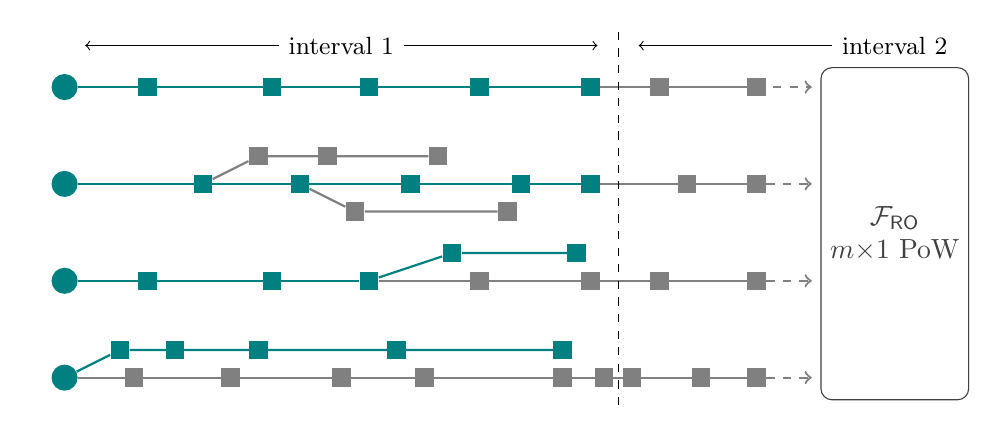
\begin{tikzpicture}
        \node (genesis) {};

        \node[fill = teal, circle] at ([xshift = 10pt, yshift = 50pt]genesis) (block11) {};
        \node[fill = teal] at ([xshift = 30pt]block11) (block12) {};
        \node[fill = teal] at ([xshift = 75pt]block11) (block13) {};
        \node[fill = teal] at ([xshift = 110pt]block11) (block14) {};
        \node[fill = teal] at ([xshift = 150pt]block11) (block15) {};
        \node[fill = teal] at ([xshift = 190pt]block11) (block16) {};
        \node[fill = gray] at ([xshift = 215pt]block11) (block17) {};
        \node[fill = gray] at ([xshift = 250pt]block11) (block1x) {};
        \draw[teal, thick] (block11) -- (block16);
        \draw[gray, thick] (block16) -- (block1x);

        \node[fill =  teal, circle] at ([xshift = 10pt, yshift = 15pt]genesis) (block21) {};
        \node[fill = teal] at ([xshift = 50pt]block21) (block22) {};
        \node[fill = teal] at ([xshift = 85pt]block21) (block23) {};
        \node[fill = teal] at ([xshift = 125pt]block21) (block24) {};
        \node[fill = teal] at ([xshift = 165pt]block21) (block25) {};
        \node[fill = teal] at ([xshift = 190pt]block21) (block26) {};
        \node[fill = gray] at ([xshift = 225pt]block21) (block27) {};
        \node[fill = gray] at ([xshift = 250pt]block21) (block2x) {};
        \draw[teal, thick] (block21) -- (block26);
        \draw[gray, thick] (block26) -- (block2x);
        \node[fill = gray] at ([xshift = 70pt, yshift = 10pt]block21) (block2f1) {};
        \node[fill = gray] at ([xshift = 95pt, yshift = 10pt]block21) (block2f2) {};
        \node[fill = gray] at ([xshift = 135pt, yshift = 10pt]block21) (block2f3) {};
        \draw[gray, thick] (block22) -- (block2f1) -- (block2f3);
        \node[fill = gray] at ([xshift = 105pt, yshift = -10pt]block21) (block2f4) {};
        \node[fill = gray] at ([xshift = 160pt, yshift = -10pt]block21) (block2f5) {};
        \draw[gray, thick] (block23) -- (block2f4) -- (block2f5);


        \node[fill =  teal, circle] at ([xshift = 10pt, yshift = -20pt]genesis) (block31) {};
        \node[fill = teal] at ([xshift = 30pt]block31) (block32) {};
        \node[fill = teal] at ([xshift = 75pt]block31) (block33) {};
        \node[fill = teal] at ([xshift = 110pt]block31) (block34) {};
        \node[fill = gray] at ([xshift = 150pt]block31) (block35) {};
        \node[fill = gray] at ([xshift = 190pt]block31) (block36) {};
        \node[fill = gray] at ([xshift = 215pt]block31) (block37) {};
        \node[fill = gray] at ([xshift = 250pt]block31) (block3x) {};
        \draw[teal, thick] (block31) -- (block34);
        \draw[gray, thick] (block34) -- (block3x);
        \node[fill = teal] at ([xshift = 140pt, yshift = 10pt]block31) (block3f1) {};
        \node[fill = teal] at ([xshift = 185pt, yshift = 10pt]block31) (block3f2) {};
        \draw[teal, thick] (block34) -- (block3f1) -- (block3f2);


        \node[fill =  teal, circle] at ([xshift = 10pt, yshift = -55pt]genesis) (block41) {};
        \node[fill = gray] at ([xshift = 250pt]block41) (block4x) {};
        \node[fill = gray] at ([xshift = 25pt]block41) (block42) {};
        \node[fill = gray] at ([xshift = 60pt]block41) (block43) {};
        \node[fill = gray] at ([xshift = 100pt]block41) (block44) {};
        \node[fill = gray] at ([xshift = 130pt]block41) (block45) {};
        \node[fill = gray] at ([xshift = 180pt]block41) (block46) {};
        \node[fill = gray] at ([xshift = 195pt]block41) (block47) {};
        \node[fill = gray] at ([xshift = 205pt]block41) (block48) {};
        \node[fill = gray] at ([xshift = 230pt]block41) (block49) {};
        \draw[gray, thick] (block41) -- (block4x);
        \node[fill = teal] at ([xshift = 20pt, yshift = 10pt]block41) (block4f1) {};
        \node[fill = teal] at ([xshift = 40pt, yshift = 10pt]block41) (block4f2) {};
        \node[fill = teal] at ([xshift = 70pt, yshift = 10pt]block41) (block4f3) {};
        \node[fill = teal] at ([xshift = 120pt, yshift = 10pt]block41) (block4f4) {};
        \node[fill = teal] at ([xshift = 180pt, yshift = 10pt]block41) (block4f5) {};
        \draw[teal, thick] (block41) -- (block4f1) -- (block4f5);

        \draw[black, dashed] ([xshift = 200pt, yshift = 20pt]block11.center) -- ([xshift = 200pt, yshift = -10pt]block41.center);
        \node at ([xshift = 100pt, yshift = 15pt]block11.center) (interval1) {\small interval 1};
        \draw[black, ->] (interval1.west) -- ([xshift = -70pt]interval1.west);
        \draw[black, ->] (interval1.east) -- ([xshift = 70pt]interval1.east);
        \node at ([xshift = 300pt, yshift = 15pt]block11.center) (interval2) {\small interval 2};
        \draw[black, ->] (interval2.west) -- ([xshift = -70pt]interval2.west);

        \node[darkgray, fill = white, draw = darkgray, rounded corners, minimum height = 120pt, align=center] at ([xshift = 50pt, yshift = -18pt]block2x) (pow) {\funcRO\\\mforone PoW};

        \draw[gray, thick, dashed, ->] (block1x.center) -- ([xshift = 20pt]block1x.center);
        \draw[gray, thick, dashed, ->] (block2x) -- ([xshift = 20pt]block2x.center);
        \draw[gray, thick, dashed, ->] (block3x) -- ([xshift = 20pt]block3x.center);
        \draw[gray, thick, dashed, ->] (block4x) -- ([xshift = 20pt]block4x.center);
    \end{tikzpicture}

    \caption{
        An illustration of the parallel blocktrees and the mining procedure.
        %
        Genesis blocks on each chain are represented as circles.
        %
        Teal blocks and forks depicts the view of a party at the end of the first interval.
        %
        There is no fork on the first chain; and on the second chain, forks are bookkeeped yet fail to revert the longest one.
        %
        The last two blocks in the view of a party on the third chain are discarded from the longest chain by another longer fork.
        %
        On the forth chain, all blocks in the first interval are reverted.
    }
    \label{fig:parallel-blocktree}
\end{figure}


\paragraph{Intervals and stages.}
%
We divide protocol time into consecutive, non-overlapping ``intervals'' in order to periodically let protocol participants adjust their local clocks and update internal states.
%
An interval consists of \syncLen rounds.
%
Parties decide which interval they are in based on their local time (thus different parties may stay in different intervals).
%
An interval is further divided into three consecutive, non-overlapping stages --- view convergence (\textsf{VC}), output generation (\textsf{OG}) and reference convergence (\textsf{RC}).
%
We denote their duration by $\syncLen_{\mathsf{VC}}$, $\syncLen_{\mathsf{OG}}$ and $\syncLen_{\mathsf{RC}}$ respectively.
%
In the view convergence (\textsf{VC}) stage, parties extend their local parallel chains and wait for the second stage.
%
Then, in the output generation (\textsf{OG}) stage, parties generate input-blocks which contain their suggested output value (cf.~\cref{subsec:new-smr-protocol}), local time (see~\cref{subsec:clock-sync-procedure}) and also interval retrieval information (see this section below).
%
They emit these input-blocks and record them on the blockchain.
%
Regarding the last stage \textsf{RC}, parties wait for a (possibly) common view of the \textsf{OG} stage and they adjust their clocks and update their internal state at the end of this stage (which is also the end of an interval).

\paragraph{A new timestamping scheme.}
%
Next, we introduce our new timestamping scheme for protocols to work with drifting clocks.
%
We extend the block timestamp from the conventional single round index $r \in  \mathbb{N}^+$ to a pair of both interval index and round index, i.e., $\protocolTime{itvl}{r} \in \mathbb{N}^+ \times \mathbb{N}^+$.
%
We say a block \block on a chain \chain is in interval $itvl$, if it reports a timestamp \protocolTime{itvl}{\cdot}.
%
A block $\block$ owns a valid timestamp iff. it satisfies the predicate $\mathsf{validTS}(r, itvl) \triangleq r \le itvl \cdot \syncLen$.
%
Note that this allows for a chain in interval $itvl$ to start with blocks reporting timestamps smaller than $(itvl - 1)\cdot \syncLen$.
%
Such adaption is necessary, since the clock adjustment algorithm might set clocks backwards; however, in the PoW setting parties must try to produce blocks in the next interval hence they should be able to mine with ``retorted'' timestamps.

Regarding blocks on the same chain (same fork on the blocktree), our protocol employs a new validation rule which asks for the monotonicity in the magnitude of stages.
%
To be precise, let $\mathsf{stage}: \mathbb{N}^+ \times \mathbb{N}^+ \rightarrow \mathbb{N}^+ \times \{ \mathsf{VC}, \mathsf{OG}, \mathsf{RC} \}$ be a function that takes a (valid) timestamp as input and outputs its corresponding stage.
%
We define a canonical order on $(itvl, stage) \in \mathbb{N}^+ \times \{ \mathsf{VC}, \mathsf{OG}, \mathsf{RC} \}$ as $(1, \mathsf{VC}), (1, \mathsf{OG}), (1, \mathsf{RC}), (2, \mathsf{VC}), (2, \mathsf{OG}), (2, \mathsf{RC}), \ldots$ so that operations like ``$<, =, \le$'' are defined canonically.
%
A chain \chain owns valid timestamps iff. for any two blocks $\block, \block'$ on \chain with timestamps \protocolTime{itvl}{r}, \protocolTime{itvl'}{r'} respectively, \block is an ancestor of $\block'$ implies $\mathsf{stage}(itvl, r) \le \mathsf{stage}(itvl', r')$.

In summary, our timestamp validation predicate, taking two consecutive blocks as input, is defined as follows.\footnote{A similar timestamping scheme with dual indices is proposed in~\cite{TCC:GarKiaShe22}. Yet their scheme still requires monotonically increasing timestamps within an interval while ours removes this restriction.}
%
\begin{equation} \label{eq:valid-timestamp-order}
      \mathsf{validOrder}(\protocolTime{itvl}{r}, \protocolTime{itvl'}{r'})
      \triangleq
      \left\{~
      \begin{aligned}
             & \textsf{validTS}(itvl, r) \wedge \textsf{validTS}(itvl', r') \\ &\wedge \mathsf{stage}(itvl, r) \le \mathsf{stage}(itvl', r')
      \end{aligned}
      \right\}.
\end{equation}
%
Note that, our blockchain notation \chainPrefixUB{\chain}{t} provides a chain with all block timestamps less than $t$, which can be ill-defined with non-monotonically increasing timestamps.
%
We stress that in our protocol we will only use this operation with a stage-boundary time (e.g., $\chainPrefixUB{\chain}{\syncLen_{\mathsf{VC}} + \syncLen_{\mathsf{OG}}}$) to get chain segments up to the end of a stage, hence resulting in an unambiguous chain.

In addition, in our protocol parties defer the processing of a chain with future timestamps until their local clocks reach that stage.
%
For instance, when the local clock of a party stays in the output generation stage of the second interval, it processes chains with blocks no later than that stage, but record all chains with blocks in the future stages for future processing.

We provide a high-level intuition behind this new timestamping scheme.
%
Suppose we stick to the conventional monotonically-increasing timestamp scheme, in our protocol analysis, an isolated success which asserts the progress of a chain should be considered with a time period of $(\delay + \maxSkew)$ rounds where $\maxSkew = \bigTheta(\syncLen)$ is the maximum skew during an interval.
%
Nonetheless, as the duration of an interval is set as a linear function of the isolated success period, this implies the clock drift \clockDrift can only be set inversely proportional to many other protocol parameters (details see our analysis).
%
With our new timestamp scheme which does not ask for the monotonicity in stages, we eliminate such correlation between clock drift \clockDrift and other protocol parameters.

\paragraph{Retrieving views from previous intervals.}
%
Recall that an interval lasts for a constant number of rounds; however the adversary can, with non-negligible probability, successfully prepare a private fork longer than the honest one that diverges up to poly-logarithmically many rounds (in $\kappa$), when the honest parties share a common view of, e.g., the first chain $\chain$ as $\parallelChains_1$ at the end of the $i$-th interval, a block \block on $\chain$ might get discarded in the future and no longer stay on the longest chain in $\parallelChains_1$.
%
(Note that \block is still bookkeeped in the blocktree, i.e., $\block \in \chain$ and $\chain \in \parallelTrees_1$.)
%
Thus, conventionally, if a party \party joins after the $i$-th interval (or, internal state of \party gets flushed after the $i$-th interval), she has no way to realize that \block is indeed in the common view on $\parallelChains_1$ at the end of the $i$-th interval.
%
This observation, at first glance, seems prohibitive for newly joint parties to catch up the internal state of existing parties, as to bootstrap they should realize the common views of honest parties at the end of each interval.

To tackle this problem, we introduce a retrieval mechanism based on Weak Agreement that allows parties to \emph{obliviously} agree on all forks that were in the common view of all honest parties at the end of each interval\footnote{Our retrieval mechanism provides no security guarantee for forks that honest parties do not share a unanimous view. Nevertheless, as we shall observe later, our protocol relies only on the oblivious agreement of honest common views.}.
%
We write $\mathtt{snapshot}_\party[i]$ to denote the set of longest chains at the end of interval $i$ in party \party's local view.
%
Note that since bad events on random oracles (e.g., two blocks share the same hash) happens with only negligible probability, $\mathtt{snapshot}_\party[i]$ can be initialized as a vector of $m$ block hashes.
%
\party bookkeeps $\mathtt{snapshot}_\party[i]$ when her local clock reaches interval $i + 1$.

During the $(i + 1)$-th interval, parties include their local view of all longest chains at the end of interval $i$ (i.e., $\mathtt{snapshot}_\party[i]$) in the input-block and emit and collect these input blocks in the output generation stage.
%
To rule out pre-mining attacks, we require each input-block \inputBlock pointing to the last block in the view convergence stage (\textsf{VC}) on its corresponding chain, thus providing fresh randomness asserting that \inputBlock is not generated too early.
%
Note that this procedure relies on parties being online at the end of the previous interval and preserve their internal state since then.
%
Recall that we assume the total computational power of corrupted parties and honest parties that suffer from transient faults (e.g., temporarily lose access to network or the RO) account for less than the majority, this guarantees that on sufficiently many parallel chains, at least half of the input blocks report local views of alert parties in the previous interval (see \cref{subsec:ro-network-corruption} for more details on party classification).

We now explain how a fresh party \newParty (either newly joining the protocol, or suffering from transient internal faults) can learn the common view of intervals in the past.
%
Our approach is simple and works in a ``trace-back'' manner:
%
For \newParty to bootstrap the blockchain and retrieve all previous views of interval $1, 2, \ldots, itvl$ where $itvl$ is the current protocol interval, \newParty first listens to the protocol passively and build parallel blocktrees.
%
\newParty then needs to decide which interval the protocol stays in (as she has no knowledge on the protocol time at this stage).
%
Given our goal to bootstrap in constant time, this is a delicate task since the adversary can gain a sudden mining success spark on all parallel chains, thus producing heaviest forks with future block timestamps in the suffix to fool the joining parties.
%
In order to eliminate such attack, after bootstrapping the blockchain, \newParty decides the interval by first pruning \kbootstr blocks on all chains and then adopt the \emph{median} block timestamp on the tip of all chains\footnote{Our analysis will show that, after pruning \kbootstr blocks, the adversary can only push forward or stall the block timestamps on a bounded fraction of chains. Hence, after adopting block timestamp that is median among all chains, \newParty learns a time that deviates from alert parties for a bounded amount of time.}.

Once \newParty is about to finish the $i$-th interval in her local view, \newParty performs the following operations recursively to retrieve the views from interval $i - 1$ to $1$.
%
Precisely, in order to set the view of a previous interval, e.g., $\mathtt{snapshot}_\party[i - 1]$, \newParty tries to find block hashes in her local parallel blocktrees that has been referred to by sufficiently many input-blocks in the next interval.
%
For the $j$-th chain, if in the $i$-th interval, there exists more than $3m / 4$ chains such that the majority of the input-blocks report the same block reference chunk \stringSegment{h'}{j}{m} (where $h'$ is a $\kappa$-bit string in input blocks to report the miner's local view of the previous interval) and a block with hash \stringSegment{h'}{j}{m} do exist in \parallelTreesLocal, then the $j$-th chunk of $\mathtt{snapshot}_\party[i - 1]$ is set to $\stringSegment{h'}{j}{m}$; otherwise (either no block hash is refereed by sufficiently many chains, or if no such block exists), it is set to $\bot$.

Note that Weak Agreement on parallel chains is not sufficient to tighten newly joint party's local clock.
%
The decision on which interval \newParty is in only gives a coarse notion of time.
%
We introduce the full bootstrapping protocol for new parties to synchronize with online ones in~\cref{subsec:clock-sync-procedure}, using the retrieval mechanism in this section as a sub-routine.
%
We also elaborate in~\cref{subsec:new-smr-protocol} on how to bootstrap the ledger state when obliviously agreeing on a large fraction of parallel chains in all intervals.

\begin{remark} \label{remark:weak-agreement}
      Our usage of Weak Agreement to retrieve previous intervals is also adopted in the bootstrapping procedure of the distributed ledger protocol in~\cite{EC:GarKiaShe24}.
      %
      Nonetheless, we stress that we adapt this technique to our new parallel blockchain construction, which achieves bootstrapping with no knowledge of time and optimal corruption resiliency with dynamic participation, which cannot be achieved by the bootstrapping algorithm in~\cite{EC:GarKiaShe24}.
\end{remark}

\paragraph{The difficulty adjustment algorithm.}
%
We adjust the mining difficulty on each chain independently, using a ``reversed'' version of Bitcoin's target recalculation function (cf.~\cite{TCC:GarKiaShe22}) which adjusts the mining target every \epochLen rounds\footnote{In Bitcoin, the mining difficulty is adjusted for every epoch of 2016 blocks.}.

In more detail, we divide time into consecutive, non-overlapping epochs and set the duration \epochLen of an epoch as a multiple of intervals so that the end of an epoch coincides with the end of an interval.
%
Note that since our timestamping scheme asks for the explicit interval indices, the epoch that a block belongs to can be directly decided based on its timestamp; and on a single chain, the epoch indices of blocks increase monotonically.
%
Epochs also apply to the blocktrees as every block on the tree must belong to a unique chain.
%
Further, parties also maintain an internal variable \epoch indicating the epoch index that they stay in.

Let $\varLambda_{\mathsf{epoch}}$ denote denote the ideal number of blocks in an epoch.
%
We have $\varLambda_{\mathsf{epoch}} = \epochLen \cdot f$, where $f$ is the ideal block generation rate.
%
For the first epoch $(\epoch = 1)$, parties adopt the same target as
the genesis block ($T_0$).
%
I.e., $T_1 = T_0$.
%
Regarding the second and later epochs $(\epoch > 1)$, parties figure out how many blocks are produced in the previous epoch, and set the next target based on the previous one.
%
This variation is proportional to the ratio of expected number of blocks $\varLambda_{\mathsf{epoch}}$ and their actual number.
%
I.e., for epoch $\epoch + 1$,
%
\begin{equation} \label{eq:target-recalc}
      T_{\epoch + 1} \triangleq \min \Big\{ \max \Big\{ \frac{\varLambda_{\mathsf{epoch}}}{\varLambda} \cdot T_{\epoch}, \frac{1}{\tau} \Big\}, \tau \Big\},
\end{equation}
%
where $\varLambda$ is the number of blocks in epoch \epoch, and $\tau$ is the bound on the relative amount of difficulty that can be adjusted each time.

In our analysis, we show that while the difficulty adjustment is performed on each chain independently, it can be set appropriately to stay close to the ideal block generation rate, thus accommodating the varying computational power.

\subsection{The Clock Synchronization Procedure}
\label{subsec:clock-sync-procedure}

\paragraph{Synchronization beacons.}
%
In the context of clock synchronization, we also call input-blocks as ``synchronization beacons'' (cf.~\cite{EC:BGKRZ21,TCC:GarKiaShe22}).
%
When parties are in the output generation (\textsf{OG}) stage of an interval \interval (in their local view), they mine beacons with their local time \protocolTime{\interval}{\round} and include all beacons (which are valid with respect to interval \interval) into their corresponding chains.
%
Note that beacons should still convey inputs for building the state machine (refer to~\cref{subsec:new-smr-protocol}) as well as local views of the previous interval to help retrieve the views and secure the parallel blockchain (\cref{subsec:new-parallel-blockchain}); for brevity we omit those details in this section.

Our shift calculation algorithm is based on comparing the timestamp recorded in beacons and their earliest local arrival time.
%
In order to perform such computation, parties need to bookkeep the time that they receive fresh beacons (in case parties receive duplicate beacons, they consider the one that arrives earliest in their local view).
%
Once a party \party receives a beacon \inputBlock (either directly or by observing it on a chain) at local time \protocolTime{\interval}{\round}, \party bookkeeps its arrival time in a local beacon registry $\mathsf{arrivalTime}(\cdot)$ as an entry $(\inputBlock, \protocolTime{\interval}{\round}, \mathrm{flag})$ where $\mathrm{flag} \in \{ \mathsf{temp}, \mathsf{final} \}$.
%
When the beacon \inputBlock is valid with respect to a fork in the parallel blocktrees in the current or previous interval, \party assigns \textsf{final} to the $\mathrm{flag}$ of \inputBlock; otherwise, it assigns \textsf{temp}.
%
Note that for a beacon \inputBlock labeled with \textsf{temp}, it will be removed from the registry when \party enters the corresponding interval and \party's local blockchain invalidates \inputBlock (invalid beacons are those that do not provide good fresh randomness with respect to any fork in party's local blocktrees).
%
Since timestamp is part of the block header, a beacon \inputBlock can be a valid one on multiple chains; yet, it suffices to bookkeep only one entry in $\mathsf{arrivalTime}(\cdot)$ and it can be reused for the same beacon in multiple chains.

A beacon \inputBlock is said to be valid with respect to an interval $itvl$ and a chain \chain, if (i) \inputBlock reports a timestamp in the \textsf{OG} stage of interval $itvl$; (ii) \inputBlock points to the last block in the \textsf{VC} stage of interval $itvl$ on \chain; and (iii) \inputBlock is a valid PoW message w.r.t. $itvl$ and \chain.
%
Refer to~\cref{algorithm:isValidInputBlock} for a full description.

\paragraph{Shift calculation algorithm.}
%
We define $\mathsf{arrivalTime}$ as a function, taking a beacon \inputBlock as input, outputs its local arrival time \protocolTime{\interval}{\round}; recall that $\mathsf{TS}$ is a function that outputs the timestamp recorded in a block \block, we slightly abuse this notation and let it take also a beacon as input.
%
We write $\inputBlock \in \chain^{(i)}$ if a beacon \inputBlock is recorded in the output generation stage of $i$-th interval on a chain \chain and \inputBlock is valid with respect to \chain.
%
When the interval index is clear in the context, we drop the superscript and simply write $\inputBlock \in \chain$.

Parties compute a value \shift at the end of an interval (i.e., when their local clock enters a round such that $\round = (\interval - 1) \cdot \syncLen$), using beacons recorded in the current interval, and adds \shift to its local time.
%
Specifically, for a party \party with local parallel chains \parallelChainsLocal at the end of interval $itvl$, its local shift $\shift_\party$ is computed as
%
\begin{equation} \label{eq:sync-shift}
    \shift_\party
    \triangleq
    \mathsf{avg} \Big( \mathsf{select} \Big( \mathsf{reduce} \Big( \Big\{ \med \Big\{ \timestamp{\inputBlock} - \mathsf{arrivalTime}(\inputBlock) \mathbin\Big| \inputBlock \in \chain \Big\} \mathbin\Big| \chain \in \parallelChainsLocal \Big\}, \eta \Big), \eta \Big) \Big).
\end{equation}
%
where $\eta < m / 2$ is a protocol parameter, and \textsf{select} and \textsf{reduce} are as defined in~\cref{eq:reduce-select}.

Roughly speaking, this algorithm can be viewed as first adjusting a party \party's local clock separately on each single chains by computing the median shift (i.e., the difference between beacon time and its local receiving time) thus yielding $m$ different clock times; then, the same decision procedure as that in~\cref{protocol:approximate-consensus} is applied on these clocks, by filtering the largest and smallest $\eta$ ones, picking the first clock time every $\eta$ remaining values, and then compute their average.

With a positive \shift at the end of interval \interval, party \party skips \shift rounds and forward her local clock to \protocolTime{\interval + 1}{\interval \cdot \syncLen + \shift}.
%
Otherwise, her clock is set backward $|\shift|$ rounds and in the next round she tries to mine a block with timestamp \protocolTime{\interval + 1}{\interval \cdot \syncLen - |\shift|} for the $(itvl + 1)$-th interval.
%
Recall our timestamping scheme in~\cref{subsec:new-parallel-blockchain}, such ``retorted'' timestamp is allowed in the view convergence stage.
%
Additionally, parties will update their beacon registry, by applying \shift on the local receiving time of all future beacons.

We note that, with overwhelming probability, every \shift value that honest parties compute at the end of each interval is well-bounded, so that their logical time stays in a good linear envelope of the nominal time, which guarantees accuracy.
%
We also prove that, when parties start an interval with bounded skew $\initSkew = \bigTheta(\clockDrift \delay)$ and certain good properties on the parallel blockchains in this interval hold, after all honest parties enter the next interval, their local clocks are at most $\maxSkew = \bigTheta(\clockDrift \delay)$ apart from each other, which solves the synchronization problem.
%
Looking ahead, our full analysis (\cref{sec:full-protocol-analysis}) will show that these good properties hold throughout the entire execution and thus all intervals serve as good synchronizers.

\paragraph{The bootstrapping procedure.}
%
We now show how a fresh party, with total lack of knowledge other than the genesis block (CRS), can join the \pSMR protocol by passively observing the protocol execution for a \emph{constant} number of rounds.
%
We highlight that even without dynamic participation, this joining procedure is still of interest as parties that passively listening to the protocol can learn a precise time in the protocol and use it as a timestamping service.
%
This procedure also allows for an existing protocol participant, whose internal state suddenly gets flushed, to catch-up with other honest parties.

Consider a newly joining party \newParty.
%
Given the interval retrieval mechanism introduced in~\cref{subsec:new-parallel-blockchain}, \newParty can bootstrap her local parallel blocktrees \parallelTreesLocal, by listening to the protocols for a constant amount of time and updating the heaviest chain such that for each interval, \newParty obliviously learns a subset of forks that are in the common view of alert parties.
%
Nonetheless, recall our timestamping scheme in~\cref{subsec:new-parallel-blockchain}, blockchains only provide a coarse notion of time such that the local clock of \newParty can deviate from alert ones for $\syncLen_{\mathsf{VC}}$ rounds.
%
Our goal is to further tighten this skew to $\maxSkew = \bigTheta(\clockDrift \delay)$ --- a small constant.

We now explain how the fresh party \newParty can synchronize with alert parties with well-bounded skews.
%
Upon executing the bootstrapping procedure, \newParty resets her local clock to \protocolTime{1}{1}.
%
During the bootstrapping phase, \newParty also listens to the beacon diffusion network $\funcDiffuse^{\textsf{input}}$ and bookkeep the arrival time of all beacons.
%
This phase lasts for more than two interval durations so that \newParty observes at least one complete output generation stage in an interval.
%
Since \newParty is not synchronized, she cannot filter any invalid beacons so she temporarily mark all beacons as \textsf{temp}.
%
Nonetheless, after she finishes bootstrapping her parallel blockchain, \newParty roughly understands which interval she stays in hence \newParty starts to remove invalid beacons based on her local heaviest chain.
%
Note that our protocol guarantees that a large fraction of chains yield good properties at the end of an interval (e.g., common view of the chain in the output generation stage), \newParty thus shares the same beacon set (marked as \textsf{final}) with alert parties on sufficiently many chains.
%
At the end of the bootstrapping procedure, by iterating all complete intervals that \newParty has observed and applying sequentially the shift calculation algorithm in~\cref{eq:sync-shift}, \newParty synchronizes her clock with all alert parties.
%
Note that when \newParty has observed two or more complete intervals, the local arrival time of all beacons in the second and later intervals needs to be updated each time after clock adjustment, by adding shift computed from the last interval to these beacons.
%
The full description of the bootstrapping procedure is presented in~\cref{protocol:joining-procedure}.

\paragraph{An improved honest-majority lower bound for clock synchronization.}
%
We discuss under what circumstances honest majority is necessary for clock synchronization.
%
Regarding corruption resiliency of synchronization problems, in the information-theoretic setting, Dolev \textit{et al.} \cite{JCSS:DHS86} show that clock synchronization is impossible when more than one-third of the parties are corrupted.
%
In the authenticated setting (assuming unforgeable signatures and a PKI), on one side, Srikanth and Toueg \cite{JACM:SriTou87} show that honest majority is necessary when the resulting linear envelope on logical time is as good as that on nominal time.
%
On the other side, Halpern \textit{et al.} \cite{PODC:HSSD84} presents a dishonest majority protocol however its logical time can deviate drastically from the real time as the number of corrupted parties grows.

We extend the argument for honest majority in~\cite{JACM:SriTou87} to a more general accuracy condition.
%
In a nutshell, when physical clocks drifts in a $(1 + \clockDrift)$-linear envelope, we show that to stay in the time that is \emph{strictly tighter} than a $(1 + \clockDrift)^2$-linear envelope of nominal time, a majority of honest parties (resources) is necessary.
%
We state this result in~\cref{thm:honest-majority-necessity}, and a depiction on the logical linear envelope where honest majority is necessary can be found in~\cref{fig:honest-majority}.

\begin{figure}[ht] \centering
    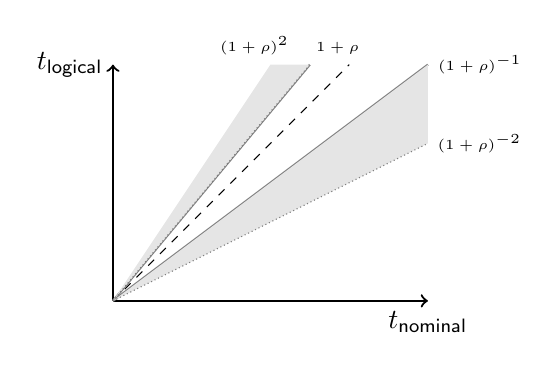
\begin{tikzpicture}
        \draw[->, thick] (0, 0) -- (4, 0) node[below] {$t_{\mathsf{nominal}}$};
        \draw[->, thick] (0, 0) -- (0, 3) node[left] {$t_{\mathsf{logical}}$};
        \draw[dashed] (0, 0) -- (3, 3);

        \draw[thick, color = gray] (0, 0) -- (4, 3) node[right, color = black] {\tiny $(1 + \clockDrift)^{-1}$};

        \draw[thick, color = gray] (0, 0) -- (2.5, 3) node[above, color = black, xshift = 1em] {\tiny $1 + \clockDrift$};

        \fill[fill = gray!20] (0, 0) -- (4, 3) -- (4, 2);
        \fill[fill = gray!20] (0, 0) -- (2, 3) -- (2.5, 3);

        \draw[densely dotted, color = gray] (0, 0)--(4, 2) node[right, color = black] {\tiny $(1 + \clockDrift)^{-2}$};
        \draw[densely dotted, color = gray] (0, 0)--(2.5, 3) node[above, color = black, xshift = -2em] {\tiny $(1 + \clockDrift)^2$};
    \end{tikzpicture}
    \caption{\sl An illustration of the logical time linear envelope (in gray) such that honest majority is necessary.}
    \label{fig:honest-majority}
\end{figure}


\begin{theorem} \label{thm:honest-majority-necessity}
    Any clock synchronization protocol running by parties with \clockDrift-linear-envelope physical clocks that achieves \maxSkew-bounded skews and $\varGamma$-accuracy such that $\maxSkew \in \mathbb{N}$ and $\clockDrift \le \varGamma < 2\clockDrift + \clockDrift^2$ must have a majority of honest parties.
\end{theorem}

\begin{proof}
    Let $D_i(r)$ denote the clock of party $\party_i$ at nominal time $r$ and $C_i(r)$ denote the (exported) logical time of party $\party_i$ at nominal time $r$.

    Assume $0 < \epsilon \ll \clockDrift$ and there exists a protocol that achieves  $((1 + \clockDrift)^{-1} (1 + \clockDrift - \epsilon)^{-1}, (1 + \clockDrift) (1 + \clockDrift - \epsilon))$-accuracy with dishonest majority.
    %
    We show that it is impossible by first considering a system with two parties $\party, \party'$ and the following three executions.
    %
    \begin{cccItemize}[noitemsep]
        \item \emph{Execution $E_1$.}
        %
        Both the parties follow the protocol, and party \party has the maximum clock speed (i.e., $D_1(r) = (1 + \clockDrift) r$); party $\party'$ has the minimum speed ($D'_1(r) = (1 + \clockDrift)^{-1} r$).
        %
        Moreover, all messages have delay exactly $\delay / (1 + \clockDrift)^2$.

        \item \emph{Execution $E_2$.}
        %
        Party \party is honest and has rate $R_2(r) = (1 + \clockDrift)^{-1} r$; party $\party'$ is corrupted and runs at $R'_2(r) = (1 + \clockDrift)^{-3} r$ but is otherwise correct.
        %
        Moreover, all messages have delay exactly \delay.

        \item \emph{Execution $E_3$.}
        %
        Party $\party'$ is honest and has rate $R'_3(r) = (1 + \clockDrift) r$; party $\party_1$ is corrupted and runs at $R_3(r) = (1 + \clockDrift)^3 r$ but is otherwise correct.
        %
        Moreover, all messages have delay exactly $\delay / (1 + \clockDrift)^4$.
    \end{cccItemize}
    %
    All these three executions follow the clock and network assumptions and are hence admissible.
    %
    In addition, executions $E_1$ and $E_2$ are indistinguishable for party \party; and executions $E_1$ and $E_3$ are indistinguishable for party $\party'$.
    %
    Since accuracy is achieved, \party in execution $E_1$ will report a time $C_1(r) \le (1 + \clockDrift)(1 + \clockDrift - \epsilon) r + b_1$.
    %
    Since $D_1(r) = (1 + \clockDrift) r$, we find that $C_1(r) \le (1 + \clockDrift - \epsilon) D_1(r) + b^1$.
    %
    Similarly, by considering execution $E_2$ we have $(1 + \clockDrift - \epsilon)^{-1} C_2(r) + a_2 \le C_2(r)$.
    %
    Since executions $E_1$ and $E_2$ are indistinguishable for party \party, the relation between its exported time and reading time must be the same in both executions.
    %
    Therefore, we have for $k = 1, 2$,
    %
    \[ (1 + \clockDrift - \epsilon)^{-1} D_k(r) + a_2 \le C_k(r) \le (1 + \clockDrift - \epsilon) D_k(r) + b_1. \]
    %
    I.e., in execution $E_1$ we can find a time $\tau_1$ such that for all $r > \tau_1$,
    %
    \[ (1 + \clockDrift - \epsilon)^{-1} (1 + \clockDrift) r + a_2 \le C_1(r) \le (1 + \clockDrift - \epsilon) (1 + \clockDrift) r + b_1. \]
    %
    Similarly, by considering party $\party'$ in executions $E_1$ and $E_3$, we see that there exist a time $\tau_2$ in execution $E_1$ such that for all $r > \tau_2$,
    %
    \[ (1 + \clockDrift - \epsilon)^{-1} (1 + \clockDrift)^{-1} r + a_1 \le C'_1(r) \le (1 + \clockDrift - \epsilon) (1 + \clockDrift)^{-1} r + b_3. \]
    %
    Hence, we find that there exist a time $\tau \ge \max \{ \tau_1, \tau_2 \}$ in execution $E_1$ such that for all $r > \tau$, the deviation between the exported time of two correct parties is greater than a constant \maxSkew, which violates the bounded skew condition.
\end{proof}

\subsection{The New State Machine Replication Protocol}
\label{subsec:new-smr-protocol}

The parallel blockchain framework that we have introduced, complemented with the clock synchronization mechanism, allow a varying number of parties to reach weak agreement sequentially at the end of each interval.
%
Based on this, we build permissionless Byzantine Agreement and state machine replication protocols.

Our approach in this section is based on the constructions in~\cite{EC:GarKiaShe24}, which provide a generic way of building BA that terminates in expected-constant time, and SMR that settles all incoming transactions in expected-constant time on top of parallel chains.
%
Their underlying parallel blockchains, however, are not truly permissionless, operate in a synchronous network and rely on a global clock, shortcomings that we overcome in this paper.

\paragraph{Permissionless BA in expected-constant time.}
%
We run ``Chain-King Consensus'' as introduced in~\cite{EC:GarKiaShe24} on top of our parallel blockchain.
%
At a high level, this protocol emulates the classical ``Phase-King Consensus'' \cite{ICALP:BerGar89,FOCS:BerGarPer89} with randomized king election \cite{PODC:FitGar03,C:KatKoo06} in the following way.

We map the $i$-th parallel chain to the $i$-th party in a classical randomized Phase-King protocol\footnote{A subtle difference compared with classical protocols is that in Chain-King Consensus, the set of chains that emulates an honest party keeps changing, while in classical protocols the set of honest parties remains the same (yet unknown). The protocol still works in that all state-update operations are based on counting the number of messages and has nothing to do with party identifiers.}.
%
For each interval, parties might share possibly different views on the output of a single chain, which emulates that parties share possibly different views on the message sent by a party in the classical protocol.
%
If a chain is good (i.e., honest parties share common views and the majority of the input blocks are honestly generated) then it emulates an honest party since its output is unanimous and validity holds.
%
Otherwise, a chain emulates a corrupted party as its output might differ among parties or validity might not hold.
%
The protocol runs in iterations by checking if parties start with the same input.
%
If this is not the case and parties are ``confused'' about the output, then they adopt the output of the king chain (set \emph{deterministically} as the first chain) as their new input (this mimics the oblivious king election in classical protocols).
%
Since the duration of intervals are of constant rounds, and the king chain yields a good chain with constant probability, the protocol terminates in expected-constant time.

In more detail, consider a BA invocation where a party \party starts with an input $v$.
%
Party \party maintains three internal variables:
%
(i) the suggestion of output $\val$ which is initialized as $v$ and can be modified at the end of each interval;
%
(ii) a bit variable \lock that indicates whether parties should take the output of king chain;
%
(iii) a bit variable \decide that indicates whether a party \party should decide on the current \val as output\footnote{Note that due to non-simultaneous termination, in~\cite{EC:GarKiaShe24}, for one-shot consensus, there is a fourth ``exit'' parameter indicating whether parties should drop from extending the blockchains. For simplicity, we avoid this part in our description and refer to~\cite{EC:GarKiaShe24} for more details.}.
%
The protocol proceeds in iterations where each iterations consists of three intervals.
%
In the first interval, parties will set both their \decide and \lock to \true if they have seen more than $3 m/ 4$ chains output the same value; and in the second interval, they set only \lock to \true if they have seen more than $3 m/ 4$ chains output the same value.
%
In both the first and second intervals, if the majority of chains output the same value, then parties will switch their \val to that output.
%
In the third interval, parties update their internal state based on \decide and \lock.
%
A party will replace \val with the output of the first (king) chain if both \decide and \lock remains \false; and it will terminate if \decide is \true;
when \decide remains \false however \lock is set to \true, it resets \lock back to \false.

A detailed description of the core state update algorithm in Chain-King Consensus is presented in~\cref{protocol:update-state-chain-king}.

\paragraph{Permissionless and self-sufficient SMR with fast fairness.}
%
Given that an invocation of permissionless BA can be run on top of our parallel chain framework, the translation to permissionless SMR works so long as (i) there are means to coordinate the second and later BA invocations that parties may start at different intervals; and (ii) an honest input is selected as output with \emph{constant} probability which guarantees liveness in expected-constant time.

At a high level, our approach here is reminiscent of that in~\cite{EC:GarKiaShe24}.
%
In order to coordinate parties that may start at different times, we employ
%
(i) the Bracha-style termination \cite{PODC:Bracha84} to let parties terminate in neighboring intervals at the end of a BA invocation;
%
and (ii) super-interval expansion (which mimics the classical super-round expansion in round-preserving sequential composition of BA \cite{JC:CCGZ19}) to allow parties expand normal interval to super-interval that consists of multiple intervals so that even if parties start non-simultaneous they still reach weak agreement on the output of this super interval.

Note that since parties in SMR use a sequence of transactions as their BA input, they are almost unlikely to start unanimously with the same set of transactions (as we will show soon, if parties also want to add the coinbase transaction, then they will never invoke BA with the same input).
%
In order to prevent the adversary from dominating the output all the time (due to the weak validity property), we proceed as follows.
%
Recall that Chain-King Consensus runs in iterations and each iteration consists of three intervals, when parties are in the first and second interval of an iteration, they decide the output of each chain as follows:
%
A party \party outputs $v$ for the $i$-th chain if the majority of input-blocks reports $v$; otherwise \party outputs $\bot$ (in this way, the adversary cannot let parties decide on a batch of transactions that is not an honest input in the first two stages).
%
When \party is in the third interval and about to switch her input, she replaces her BA input with the input-block of smallest hash value in the king chain.

We now show how parties can build an ever-growing log with fast fairness.
%
Once a block (a sequence of transactions from the BA output) is appended to the log in SMR, it sets up a public key $\mathsf{pk}$ such that the probability that $\mathsf{pk}$ belongs to an honest party is roughly proportional to the fraction of her computational among all protocol participants.
%
Upon joining the protocol, a party \party generates her own public-key pair $(\mathsf{pk}, \mathsf{sk})$ as her identifier (pseudonym).
%
Recall that our SMR is built on the sequential composition of BA invocations, and in each invocation parties prepare their own input using all unsettled transactions in their buffer.
%
We additionally introduce the following mechanism.

At the onset of a BA invocation, \party prepares a special transaction $\tx^{\text{base-tx}}$ that contains her public key $\mathsf{pk}$.
%
\party then appends all valid, unsettled transactions in the buffer after $\tx^{\text{base-tx}}(\mathsf{pk})$ as her BA input.
%
Moreover, we add an additional interval at the beginning of BA such that at the end of this interval, parties listen to the king chain and switch their \val to the block with minimum hash.
%
As a result, the output of each BA in our SMR protocol is a sequence of transactions, with the first transaction being coinbase of public key $\mathsf{pk}$.

Next, we provide some intuition on how the above mechanism helps to achieve fast fairness (refer to~\cref{sec:full-protocol-analysis} for more details).
%
We focus on the first interval which serves as a ``lottery''  letting parties replace their input with the block with minimum hash.
%
Suppose parties share a common view on the king chain until the end of that interval, if an honest party manages to produce an input-block with the minimum hash among all parties, this implies that she makes a RO query such that the RO response yields minimum among all hash queries made that can contribute to the king chain (that is, the output generation stage of that interval).
%
Also note that an input-block with minimum hash will be a valid block on the king chain (since it is definitely smaller than the mining target $T$).
%
Hence, the probability that a party wins the lottery is the same as winning the minimum block hash on king chain, and is (roughly) proportional to her computational power among all participants.
%
Even though the adversary can gain some bounded advantage by slightly cheating on the block timestamp, yet, since the honest parties share a common view of the king chain, the adversary can only keep including more input-blocks with bogus timestamps for a bounded amount of time.
%
In case the king chain is a bad chain, all bets are off.
%
Nonetheless, our analysis shows that the protocol can be parameterized so that the probability that the king chain is a bad chain is an arbitrarily small constant.
%
Combining these two bounded, constant errors together, we can conclude that whenever a new batch of transactions is to be appended to the SMR log, the probability a party gets selected is proportional to her relative computational power.

\subsection{Full Protocol Description}
\label{subsec:full-protocol-description}

\paragraph{Main protocol instance.}
%
We introduce the main \pSMR protocol instance that dispatches to the relevant subprocesses following the UC notions.

\begin{cccProtocol}
    {$\pSMR(\party, \sid; \funcDriftingClock, \funcRO, \funcDiffuse, \funcCRS)$}
    {main-protocol}
    {The main protocol instance of \pSMR.}

    \paragraph{Global Variables:}
    %
    \begin{cccItemize}[nosep]
        \item Read-only: \syncLen, \epochLen, $t_{\mathsf{off}}$, $t_{\mathsf{gather}}$

        \item Read-write: \localTime, \epoch, \parallelChainsLocal, \parallelTreesLocal, $T^{\epoch}$, $\mathtt{isInit}$, $t_{\mathsf{work}}$, \buffer, \inputBlockBuffer, \futureChains, \isSync, \fetchCompleted, $\mathsf{arrivalTime}(\cdot)$, \state, $\mathtt{snapshot}$
    \end{cccItemize}

    \paragraph{Registration / Deregistration:}
    %
    \begin{cccItemize}[nosep]
        \item Upon receiving input $(\textsc{register}, \mathcal{R})$, where $\mathcal{R} \in \{\funcLedger, \funcDriftingClock \}$ execute protocol $\mathsf{Registration}(\party,\allowbreak \sid, \mathtt{reg}, \mathcal{R})$.

        \item  Upon receiving input $(\textsc{de-register}, \mathcal{R})$, where $\mathcal{R} \in \{\funcLedger, \funcDriftingClock \}$ execute protocol $\mathsf{Deregistration}(\party, \sid,\allowbreak \mathtt{reg}, \mathcal{R})$.

        \item Upon receiving input $(\textsc{is-registered}, \sid)$ return $(\textsc{register}, \sid, 1)$ if the local registry $\mathtt{Reg}$ indicates that this party has successfully completed a registration with $\mathcal{R} = \funcLedger$ (and did not de-register since then).
        %
        Otherwise, return $(\textsc{register}, \sid, 0)$.
    \end{cccItemize}

    \paragraph{Interacting with the Ledger:}
    %
    Upon receiving a ledger-specific input $I \in \{(\textsc{submit}, \ldots), \allowbreak (\textsc{read}, \ldots), \allowbreak (\textsc{maintain-ledger}, \ldots) \}$ verify first that all resources are available.
    %
    If not all resources are available, then ignore the input; else (i.e., the party is operational and time-aware) execute one of the following steps depending on the input $I$:
    %
    \begin{cccItemize}[nosep]
        \item \textbf{If} $I = (\textsc{submit}, \sid, \tx)$ \textbf{then} set $\buffer \gets \buffer \concat \tx$, and send $(\textsc{diffuse}, \sid, \tx)$ to $\funcDiffuse^{\textsf{tx}}$.

        \item \textbf{If} $I = (\textsc{maintain-ledger}, \sid, \mathrm{minerID})$ \textbf{then} invoke protocol $\mathsf{LedgerMaintenance}(\party, \sid)$; \textbf{if} $\mathsf{LedgerMaintenance}$ halts \textbf{then} halt the protocol execution (all future input is ignored).

        \item \textbf{If} $I = (\textsc{read}, \sid)$ then invoke protocol $\mathsf{ReadState}(\party, \sid)$.

        \item \textbf{If} $I = (\textsc{export-time}, \sid)$ then do the following: if \isSync or $\mathtt{isInit}$ is false, then return $(\textsc{export-time}, \sid, \bot)$; otherwise call $\mathsf{UpdateLocalTime}(\party, \sid)$ and return $(\textsc{export-time}, \sid, \localTime)$ to the caller.
    \end{cccItemize}

    \paragraph{Handling calls to the shared setup:}
    %
    \begin{cccItemize}[nosep]
        \item Upon receiving $(\textsc{clock-tick}, \sid_C)$, forward it to \funcDriftingClock and output \funcDriftingClock's response.

        \item Upon receiving $(\textsc{clock-update}, \sid_C)$, record that a \textsc{clock-update} was received in the current round.
        %
        If the party is registered to all its setups, then do nothing further.
        %
        Otherwise, do the following operations before concluding this round:
        %
        \begin{enumerate}[label=\arabic*,leftmargin=*, nosep]
            \item If this instance is currently time-aware but otherwise stalled or offline, then call $\mathsf{UpdateLocalTime}(\party, \sid)$ to update \localTime.
                  %
                  If the party has passed a synchronization slot, then set $\isSync \gets \false$.

            \item If this instance is only stalled but $\isSync = \true$, then additionally execute $\mathsf{FetchInformation}(\party, \sid)$, extract all new input blocks (synchronization beacons) $IB$ from the fetched chains and record their arrival times and set $\fetchCompleted \gets \true$.
                  %
                  Also, any unfinished interruptible execution of this round is marked as completed.

            \item Forward $(\textsc{clock-update}, \sid_C)$ to \funcDriftingClock to finally conclude the round.
        \end{enumerate}
    \end{cccItemize}
\end{cccProtocol}

\paragraph{Registration / de-registration.}
%
In order to perform basic operations, a party \party needs to register to all resources.
%
Note that the protocol will initialize local time $\party.\localTime$ to \protocolTime{1}{1}, and \party is aware whether he is not synchronized not and will set the bit variable \isSync correspondingly.

\begin{cccProtocol}
    {$\mathsf{Registration}(\party, \sid, \mathtt{Reg}, \mathcal{G})$}
    {registration}
    {Parties register on necessary resources (functionalities) to run the protocol.}

    \begin{algorithmic}[1]
        \oneLineIf{$\mathcal{G} = \funcDriftingClock$}{send $(\textsc{register}, \sid)$ to $\mathcal{G}$, set registration status to registered with $\mathcal{G}$, and output the valued received by $\mathcal{G}$.}

        \If{$\mathcal{G} = \funcLedger$}

        \If{\party is not registered with \funcDriftingClock or already registered with all setups}

        \State{ignore this input}

        \Else

        \State{Send $(\textsc{clock-tick}, \sid_C)$ to \funcDriftingClock and receive $(\textsc{clock-tick}, \sid_C , \mathrm{tick})$}

        \State{Send $(\textsc{register}, \sid)$ to \funcDiffuse}

        \State{$\localTime \gets \protocolTime{1}{1}$ and $\isSync \gets \false$}

        \State{If this is the first registration invocation for this ITI, then set $\mathtt{isInit} \gets \false$.}

        \State{Output $(\textsc{register}, \sid, \party)$ once completing the registration with all the above resources \func}
        \EndIf
        \EndIf
    \end{algorithmic}
\end{cccProtocol}

The deregistration process is an analogous action that sets variables to the initial values.

\begin{cccProtocol}
    {$\mathsf{Deregistration}(\party, \sid, \mathtt{Reg}, \mathcal{G})$}
    {deregistration}
    {Parties de-register from corresponding resources.}

    \begin{algorithmic}[1]
        \If{$\mathcal{G} = \funcDriftingClock$}

        \State{Set $\isSync \gets \false$}

        \State{Send $(\textsc{de-register}, \sid)$ to $\mathcal{G}$ and set registration status as de-registered with $\mathcal{G}$}

        \State{Output the valued received by $\mathcal{G}$}

        \EndIf

        \If{$\mathcal{G} = \funcLedger$}

        \State{Set $\isSync \gets \false$}

        \State{Send $(\textsc{de-register}, \sid)$ to \funcDiffuse, set its registration status as de-registered with \funcDiffuse and output $(\textsc{de-register}, \sid, \party)$.}
        \EndIf
    \end{algorithmic}
\end{cccProtocol}

\paragraph{Ledger maintenance.}
%
The protocol $\mathsf{LedgerMaintenance}$ groups all the steps regarding the main ledger operation.
%
Note that, depending on a party is alert or not, she might execute different sub protocols.
%
For parties that are not synchronized, after querying \funcCRS, they first enter the bootstrapping mode by calling $\mathsf{JoiningProcedure}$.
%
By executing this sub protocol, they set their internal state \isSync to true and then start to execute the normal ledger maintenance operations.

\begin{cccProtocol}
    {$\mathsf{LedgerMaintenance}(\party, \sid)$}
    {ledger-maintenance}
    {The main operations for parties to maintain the ledger.}

    \begin{algorithmic}[1]
        \LineComment{The following steps are executed in an $(\textsc{maintain-ledger}, \sid, \mathrm{minerID})$-interruptible manner:}

        \If{$\mathtt{isInit} = \false$}
        \State{Send $(\textsc{Retrieve, \sid})$ to \funcCRS and set response as \textsf{CRS} and set $\mathtt{isInit} \gets \true$.}
        \EndIf

        \LineComment{Bootstrap if not synchronized.}
        \oneLineIf{\textbf{not} \isSync}{Call $\mathsf{JoiningProcedure}(\party, \sid)$}
        \Comment{\cref{protocol:joining-procedure}}

        \LineComment{Normal operations when alert.}

        \State{Invoke $\mathsf{FetchInformation}(\party, \sid)$ and denote the output by $(\chain_1, \ldots, \chain_N)$, $(\tx_1, \ldots, \tx_k)$}
        \State{$\buffer \gets \buffer \concat (\tx_1, \ldots, \tx_k)$ and $\futureChains \gets \futureChains \cup \{ \chain_1, \ldots, \chain_N \}$}

        \State{Call $\mathsf{UpdateLocalTime}(\party, \sid)$}
        \Comment{\cref{protocol:update-local-time}}

        \LineComment{Ensures the processing of new input-blocks arrived in chains only.}
        \State{Extract input-blocks $IB \gets \{ \inputBlock_1, \ldots , \inputBlock_n \}$ contained in $\chain_1, \ldots, \chain_N$ and not yet contained in \inputBlockBuffer.}

        \State{Call $\mathsf{ProcessInputBlocks}(P, \sid, IB)$}
        \Comment{\cref{protocol:process-input-blocks}}

        \State{Let $\mathcal{N}_0$ be a set of (single) chains s.t. $\chain \in \mathcal{N}_0 :\Leftrightarrow \chain \in \parallelChains \in \futureChains \wedge \forall \block \in \chain : \timestamp{\block} \le \localTime$}

        \State{Remove each $\chain \in \mathcal{N}_0$ from \futureChains}

        \State{$\fetchCompleted \gets \true$}

        \State{Call $\mathsf{UpdateLocalChain}(\parallelChainsLocal, \parallelTreesLocal, \mathcal{N}_0)$ to update \parallelChainsLocal and \parallelTreesLocal}

        \If{$t_{\mathsf{work}} < \localTime$}
        \State{Call $\mathsf{MiningProcedure}(\party, \sid, r)$}
        \Comment{\cref{protocol:mining-procedure}}

        \If{$\round = \interval \cdot \syncLen$}
        \State{Call $\mathsf{StateUpdate}(\party, \sid)$}
        \Comment{\cref{protocol:update-state}}
        \State{Call $\mathsf{SyncProcedure}(\party, \sid)$}
        \Comment{\cref{protocol:sync-procedure}}
        \EndIf

        \State{Set $t_{\mathsf{work}} \gets \localTime$}

        \EndIf

        \State{Call $\mathsf{FinishRound}(\party)$}
        \Comment{Mark normal round actions as finished}
    \end{algorithmic}
\end{cccProtocol}


\paragraph{Fetch information.}
%
Parties fetch block information from $\funcDiffuse^{\textsf{bc}}$ to learn new parallel chains (precisely, blocktrees) with possibly future timestamps.
%
Note that in order to simplify the chain validation and selection procedure, we let $\mathsf{FetchInformation}$ return all single chains $\chain_1, \ldots, \chain_N$ extracted from all received blocktrees\footnote{Parties associate all blocktrees/chains with their index $i \in [m]$ in parallel chains(trees), and thus apply chain validation and validation for chains with the same index. For brevity, we ignore these details in our protocol description and assume all chains are processed correspondingly.}.
%
Parties also fetch transactions from $\funcDiffuse^{\textsf{tx}}$ to learn new transactions.

\begin{cccProtocol}
    {$\mathsf{FetchInformation}(\party, \sid)$}
    {fetch-information}
    {Fetching new blocks and transactions from the diffusion functionality.}

    \begin{algorithmic}[1]
        \oneLineIf{\fetchCompleted}{\Return}
        \Comment{Fetch once per round and never catch up missed round.}

        \LineComment{Fetch blocks on $\funcDiffuse^{\textsf{bc}}$}

        \State{Send $(\textsc{fetch}, \sid)$ to $\funcDiffuse^{\textsf{bc}}$; denote the response by $(\textsc{fetch}, \sid, bc)$.}

        \State{Extract blocktrees $\blockTree_1, \ldots \blockTree_n$ from $bc$}

        \State{Extract chains $\chain_1, \ldots \chain_N$ from $\blockTree_1, \ldots \blockTree_n$}

        \LineComment{Fetch transactions on $\funcDiffuse^{\textsf{tx}}$}

        \State{Send $(\textsc{fetch}, \sid)$ to $\funcDiffuse^{\textsf{tx}}$; denote the response by $(\textsc{fetch}, \sid, tx)$.}

        \State{Extract transactions $(\tx_1, \ldots \tx_k)$ from $tx$}

        \If{\textbf{not} \isSync or \party is stalled}
        \State{$\buffer \gets \buffer \concat (\tx_1, \ldots \tx_k)$}
        \State{$\futureChains \gets \futureChains \cup \{ \parallelChains_1, \ldots \parallelChains_N \}$}
        \EndIf
    \end{algorithmic}

    \textsc{Output:} The protocol outputs $(\chain_1, \ldots , \chain_N)$ and $(\tx_1, \ldots, \tx_k)$ to its caller (but not to \Z).
\end{cccProtocol}

\paragraph{Chain and input block validation.}
%
We present the chain and input block validation procedure in \pSMR respectively.
%
Note that, different from the single chain protocols where the validity of each chain can be attested independently, chains in \pSMR need to be verified per interval (see the chain selection procedure in~\cref{algorithm:update-local-chain}).
%
Hence the algorithm $\mathsf{IsValidChain}$ takes as input a chain \chain, an integer $i$ the index of \chain in parallel chains, a parallel blocktree \parallelTrees that \chain is associate with and an integer $itvl$ the target interval on \chain to be verified.

The blocks (input-blocks) in \pSMR are of form
%
\[ \block = \langle ctr, \protocolTime{itvl}{r}, h, st, h^\ast, h', val \rangle, \]
%
where $ctr$ is the nonce for PoW, \protocolTime{itvl}{r} shows the block timestamp, $h$ is the hash pointer to the previous block, $st$ represents the block content (note that $h$ and $st$ are meaningful only for a block \block), $h^\ast$ is the fresh randomness when mining input-blocks, and $h', val$ is the chain reference for previous intervals (cf.~\cref{subsec:new-parallel-blockchain}) and input-block content respectively.

The following functions help us simplify the validation process:
%
\begin{cccItemize}[noitemsep]
    \item We use \textsf{ValidBlock} to verify if a block is a successful PoW on the $i$-th chain (that is, the nonce $ctr$ is valid and the block hash --- $i$-th segment of the RO output is less than target $T$).
    %
    \[ \mathsf{ValidBlock}(\block, i, T) \triangleq \stringSegment{H(\block)}{i}{m} < T \wedge \block.ctr < 2^{32}. \]

    \item Analogously, we use use \textsf{ValidInputBlock} to verify if a synchronization beacon is a successful PoW on its associated chain by checking the reverse of the string segment.
    %
    I.e.,
    %
    \begin{equation*}
        \mathsf{ValidInputBlock}(\inputBlock, i, T) = \stringSegmentRev{H(\inputBlock)}{i}{m} < T \wedge \inputBlock.ctr < 2^{32}
    \end{equation*}

    \item We adopt \textsf{isStageOG} as a predicate to justify if a timestamp $r$ is in the output generation stage of interval $itvl$.
    %
    Precisely,
    %
    \begin{equation*}
        \mathsf{isStageOG}(itvl, r) \triangleq r \in [(itvl - 1) \cdot \syncLen + \syncLen_{\mathsf{VC}}, itvl \cdot \syncLen - \syncLen_{\mathsf{RC}}].
    \end{equation*}
\end{cccItemize}

Given the above, \cref{algorithm:isvalidchain} presents a full specification of the chain validation procedure.

\begin{cccAlgorithm}
    {$\mathsf{IsValidChain}(\chain, i, \parallelTrees, itvl)$}
    {isvalidchain}
    {The chain validation procedure.}

    \newcommand*{\goodHash}{\mathEnv{\mathsf{goodHash}}}
    \newcommand*{\goodNonce}{\mathEnv{\mathsf{goodNonce}}}
    \newcommand*{\goodTime}{\mathEnv{\mathsf{goodTime}}}
    \newcommand*{\goodInputBlock}{\mathEnv{\mathsf{goodInputBlock}}}
    \newcommand*{\goodCRS}{\mathEnv{\mathsf{goodCRS}}}

    \begin{algorithmic}[1]
        \LineComment{This algorithm has five internal Boolean variables \goodHash, \goodNonce, \goodTime, \goodCRS and \goodInputBlock, all initialized as \true.}

        \oneLineIf{\chain starts with a block with hash reference other than $\mathsf{CRS}$}{$\goodCRS \gets \false$}

        \oneLineIf{\isSync \textbf{and} $\exists \block \in \chain$ s.t. $\mathsf{validOrder}(\timestamp{\block}, \localTime) = \false$}{$\goodTime \gets \false$}

        \LineComment{Derive fresh randomness for $itvl$ as indicated by \chain}
        \State{Extract $h^\ast_{itvl}$ from $\chainHead{\chainPrefixUB{\chain}{(itvl - 1) \cdot \syncLen + \syncLen_{\mathsf{VC}}}}$}

        \For{each block \block in \chain from interval $itvl$}

        \State{Parse \block as $\langle ctr, \protocolTime{itvl}{r}, h, st, \cdot, \cdot, \cdot \rangle$}

        \State{Set $T_\block \gets \mathsf{ExtractMiningTarget}(\chain, \lceil itvl / (\epochLen / \syncLen) \rceil)$.}
            \Comment{Extract mining difficulty set for \block}

            \LineComment{Check hash}
            \State{Let $\block^{-1}$ be the last block in \chain before \block}
            \State{Set $\goodHash \gets (\stringSegment{h}{i}{m} = \stringSegment{H(\block^{-1})}{i}{m})$}

            \LineComment{Check nonce}
            \State{Set $\goodNonce \gets \mathsf{ValidBlock}(\block, i, T_\block)$}

            \LineComment{Check input blocks}

            \If{$\neg \mathsf{isStageOG}(itvl, r)$ \textbf{and} $\exists \inputBlock \in \block$}
            \State{Set $\goodInputBlock \gets \false$}
            \Comment{Block should include \inputBlock only in \textsf{OG}}
            \Else

            \For{each input block $\inputBlock \in \block$}
            \State{Parse \inputBlock as $\langle ctr', \protocolTime{itvl'}{r'}, \cdot, \cdot, h^\ast_\inputBlock, \cdot, \cdot \rangle$}

            \oneLineIf{$\mathsf{isStageOG}(itvl, r) = \false$ \textbf{or} $\timestamp{\inputBlock} > \timestamp{\block}$}{$\goodInputBlock \gets \false$}

            \oneLineIf{\chain contains duplicate \inputBlock \textbf{or} $\stringSegment{h^\ast_\inputBlock}{i}{m} \neq \stringSegment{h^\ast_{itvl}}{i}{m}$}{$\goodInputBlock \gets \false$}

            \State{Set $T_\inputBlock \gets \mathsf{ExtractMiningTarget}(\chain, \lceil itvl' / (\epochLen / \syncLen) \rceil)$.}
        \State{Set $\goodInputBlock \gets \mathsf{ValidInputBlock}(\inputBlock, i, T_{\inputBlock})$}

        \EndFor

        \EndIf

        \EndFor

        \oneLineIf{$\goodHash \wedge \goodNonce \wedge \goodInputBlock \wedge \goodTime \wedge \goodCRS$}{\Return \true}
        \State{\Return \false}
    \end{algorithmic}
\end{cccAlgorithm}

Regarding input blocks that have not yet been included in chains, the validity of an \inputBlock with respect to a chain index $i$ is checked only when the party's local time has forwarded to at least the same interval as \inputBlock (if not, this procedure returns ``undecided'' which defers the validity check).

\begin{cccAlgorithm}
    {$\mathsf{IsValidInputBlock}(\inputBlock, \chain, i, \parallelTrees)$}
    {isValidInputBlock}
    {The input-block validation procedure.}

    \begin{algorithmic}[1]
        \LineComment{Precondition: Chain \chain is valid. Returns \true if the beacon is a valid beacon w.r.t. \chain, $\mathsf{undecided}$ if no judgement is possible, and \false if the beacon is invalid w.r.t. \chain.}

        \State{Parse \inputBlock as $\langle ctr, \protocolTime{itvl}{r}, \cdot, \cdot, h^\ast_\inputBlock, \cdot, \cdot \rangle$}

        \oneLineIf{\chain contains no block in interval $itvl$}{\Return $\mathsf{undecided}$}
        \Comment{no judgement possible}

        \LineComment{Check nonce value and freshness}
        \State{Extract $h^\ast_{itvl}$ from $\chainHead{\chainPrefixUB{\chain}{(itvl - 1) \cdot \syncLen + \syncLen_{\mathsf{VC}}}}$}
        \State{Set $T_\inputBlock \gets \mathsf{ExtractMiningTarget}(\chain, \lceil itvl / (\epochLen / \syncLen) \rceil)$.}
        \oneLineIf{$\mathsf{ValidInputBlock}(\inputBlock, i, T_{\inputBlock}) = \true$ \textbf{and} $\stringSegment{h^\ast_\inputBlock}{i}{m} \neq \stringSegment{h^\ast_{itvl}}{i}{m}$}{\Return \true}

        \State{\Return \false}
    \end{algorithmic}
\end{cccAlgorithm}

\paragraph{Extract mining target.}
%
We adopt algorithm $\mathsf{ExtractMiningTarget}$ to calculate the mining difficulty set for an epoch index $ep$ on a single chain \chain.
%
Starting from the initial target $T_0$, this algorithm iteratively calculates targets from the first epoch to the targeted one, based on the number of blocks in each epoch and \cref{eq:target-recalc}.

\begin{cccAlgorithm}
    {$\mathsf{ExtractMiningTarget}(\chain, ep)$}
    {extract-mining-target}
    {Extracting the mining target for a given epoch.}

    \begin{algorithmic}[1]
        \oneLineIf{$ep = 1$}{\Return $T_0$} \Comment{Return initial target}
        \For{$i$ \textbf{from} $2$ to $ep$}
        \State{$\varLambda_i = |\{ \block \mathbin| \block \in \chain \wedge \lceil \timestamp{\block} / (\epochLen / \syncLen) \rceil = i \}|$}

        \State{$T_i = \min \{ \max \{ \varLambda_{\mathsf{epoch}} / \varLambda_i \cdot T_{i - 1}, 1 / \tau \}, \tau \}$}
        \Comment{\cref{eq:target-recalc}}
        \EndFor
        \State{\Return $T_{ep}$}
    \end{algorithmic}
\end{cccAlgorithm}

\paragraph{Update local time.}
%
Parties will send \textsc{clock-tick} to \funcDriftingClock to check if it receives a $\mathrm{tick} = 0$, which indicates the beginning of a new (local) round.

\begin{cccProtocol}
    {$\mathsf{UpdateLocalTime}(\party, \sid)$}
    {update-local-time}
    {Parties update their local clock due to \funcDriftingClock.}
    
    \begin{algorithmic}[1]
        \LineComment{Precondition: Only executed if time-aware.}
        \State{Send $(\textsc{clock-tick}, \sid)$ to \funcDriftingClock and receive $(\textsc{clock-tick}, \sid , \mathrm{tick})$}

        \If{$\mathrm{tick} = 0$}
        \State{$\localTime \gets \localTime + 1$}
        \State{$\fetchCompleted \gets \false$}
        \EndIf
        \State{$\epoch \gets \lceil \interval / (\epochLen / \syncLen) \rceil$}
    \end{algorithmic}

    \textsc{Output:} The protocol outputs \localTime, \epoch to its caller (but not to \Z)
\end{cccProtocol}

\paragraph{Process input blocks and arrival times.}
%
The following procedure processes incoming input blocks, bookkeeps their arrival times and filters out duplicate ones.
%
The predicate to verify input-block validity is presented in~\cref{algorithm:isValidInputBlock}.
%
Regarding the duplicate beacons, only one with the earliest arrival time will be preserved.

\begin{cccProtocol}
    {$\mathsf{ProcessInputBlocks}(\party, \sid, IB)$}
    {process-input-blocks}
    {Parties filter invalid input blocks.}

    \begin{algorithmic}[1]
        \oneLineIf{$\fetchCompleted = \true$}{\Return}

        \State{Send $(\textsc{fetch}, \sid)$ to $\funcDiffuse^{\textsf{input}}$ and denote the response by $(\textsc{fetch}, \sid, b)$}

        \State{Extract all received input blocks $(\inputBlock_1, \ldots , \inputBlock_k)$ contained in $b \cup IB$.}

        \For{each $\inputBlock_i$ with $\mathsf{arrivalTime}(\inputBlock) = \bot$}
        \State{$\inputBlockBuffer \gets \inputBlockBuffer \cup \{ \inputBlock \}$}

        \State{Parse $\timestamp{\inputBlock}$ as \protocolTime{itvl'}{r'}}

        \If{$\isSync \wedge (\interval \ge itvl')$}

        \State{Set $\mathsf{arrivalTime}(\inputBlock_i) \gets (\localTime, \mathsf{final})$}
        \Comment{The measurement is final.}

        \Else \Comment{Will be adjusted upon next time shift.}
        \State{$\mathsf{arrivalTime}(\inputBlock_i) \gets (\localTime, \mathsf{temp})$}

        \EndIf
        \EndFor

        \LineComment{Buffer cleaning.}

        \If{\isSync}

        \For{each $\inputBlock \in \inputBlockBuffer$}

        \oneLineIf{\timestamp{\inputBlock} has timestamp later than \interval}{skip \inputBlock}

        \State{$\mathsf{goodInputBlock} \gets \false$}

        \For{$i$ \textbf{from} $1$ \textbf{to} $m$}

        \oneLineIf{$\exists \chain \in \parallelTreesLocal$ s.t. $\mathsf{IsValidInputBlock}(\inputBlock, \chain, i, \parallelTreesLocal) = \true$}{$\mathsf{goodInputBlock} \gets \true$}

        \EndFor

        \oneLineIf{$\mathsf{goodInputBlock} = \false$}{Remove \inputBlock from \inputBlockBuffer}

        \EndFor

        \EndIf
    \end{algorithmic}

    \textsc{Output:} The protocol outputs \ok to its caller (but not to \Z).
\end{cccProtocol}

\paragraph{Chain selection.}
%
Our chain selection rule (which should only be used by time-aware parties) works in two steps.
%
First, it filters all invalid chains, by verifying them in an interval-by-interval fashion.
%
I.e., chains are split into intervals and the $(i + 1)$-th interval is checked after the $i$-th interval of all chains has been checked.
%
An invalid chain $\chain^*$ is removed out of the chain buffer once any interval of $\chain^*$ fails the $\mathsf{IsValidChain}$ verification.
%
And all valid chains are added to \parallelTrees as a fork (we do this interval-by-interval as well).
%
After filtering all invalid chains, the next step runs the chain selection procedure for every chain index in the current interval, and replaces each chain in \parallelChains with the longest fork in the corresponding tree in \parallelTrees.

\begin{cccAlgorithm}
    {$\mathsf{UpdateLocalChain}(\parallelChains, \parallelTrees, \mathcal{N}_0 = \{ \chain_1, \ldots, \chain_N \})$}
    {update-local-chain}
    {Parties filter invalid chains and select the heaviest one.}

    \begin{algorithmic}[1]
        \LineComment{This algorithm should only be called by fully-synchronized parties.}

        \For{$itvl$ \textbf{from} $1$ \textbf{to} \interval}
        \For{each $\chain \in \mathcal{N}_0$}
        \State{Let $i$ be the chain index of \chain}
        \If{$\mathsf{IsValidChain}(\chain, i, \parallelTrees, itvl) = \true$}
        \State{Add $\chainPrefixUB{\chain}{itvl \cdot \syncLen}$ to the $i$-th tree in \parallelTrees}
        \Else \Comment{invalid chain from $itvl$}
        \State{Remove \chain from $\mathcal{N}_0$}
        \EndIf
        \EndFor
        \EndFor

        \For{$i$ \textbf{from} $1$ \textbf{to} $m$}
        \State{Set $\chain_{\mathrm{max}} \gets \parallelChains_i$}
        \For{each $\chain \in \parallelTrees_i$}
        \oneLineIf{$\chainDiff{\chain} > \chainDiff{\chain_{\mathrm{max}}}$}{$\chain_{\mathrm{max}} \gets \chain$}
        \EndFor
        \State{Replace the $i$-th chain in \parallelChains by $\chain_{\mathrm{max}}$}
        \EndFor

        \State{\Return $\parallelChains, \parallelTrees$}
    \end{algorithmic}
\end{cccAlgorithm}

\paragraph{Mining procedure.}
%
Once a party \party has prepared all information and updated its state, she can run the core mining procedure in~\cref{protocol:mining-procedure}.
%
When \localTime reports in the output generation phase, \party will include the fresh input blocks and check if she succeeds in the input-block mining procedure.
%
At the onset of a BA invocation (when internal variable \val is set to $\bot$), \party starts to build her own input, starting from a coinbase transaction $\tx_\party^{\text{base-tx}}$ that contains her public key $\mathsf{pk}$ and she also signs this transaction.

Note that, for simplicity, we adopt two functions \blockify and $\mathsf{ValidTx}$ (cf.~\cite{C:BMTZ17}) that translates a sequence of transactions to the ledger state and verifies an incoming transaction w.r.t. a ledger state respectively, which we omit the details.

\begin{cccProtocol}
    {$\mathsf{MiningProcedure}(\party, \sid)$}
    {mining-procedure}
    {The mining procedure of $m$ parallel blocks/input-blocks.}

    \begin{algorithmic}[1]
        \LineComment{The following steps are executed in an (maintain-ledger, sid, minerID)-interruptible manner:}


        \State{$h \gets \varepsilon$}
        \Comment{Prepare chain head}

        \For{$i$ \textbf{from} $1$ \textbf{to} $m$}
        \State{Parse the last block of $i$-th chain in \parallelChainsLocal as \block}
        \Comment{Possibly genesis block (CRS)}
        \State{$h \gets h \concat \stringSegment{H(\block)}{i}{m}$}
        \EndFor


        \If{$\mathsf{isStageOG}(\localTime)$}

        \State{Set $h^\ast \gets \varepsilon$ and $st \gets \varepsilon$}

        \LineComment{Prepare fresh randomness}
        \For{$i$ \textbf{from} $1$ \textbf{to} $m$}
        \State{Parse the last block in the \textsf{VC} stage of $i$-th chain in \parallelChainsLocal as \block}
        \State{$h^\ast \gets h^\ast \concat \stringSegment{H(\block)}{i}{m}$}
        \EndFor

        \LineComment{Prepare block content}
        \State{$\mathbf{N} \gets \varepsilon$}
        \For{$i$ \textbf{from} $1$ \textbf{to} $m$}
        \State{Parse the $i$-th chain in \parallelChainsLocal as \chain}
        \State{Set $IB \gets \{\inputBlock' \in \inputBlockBuffer \mathbin| \mathsf{IsValidInputBlock}(\inputBlock', \chain, i, \parallelTreesLocal) = \true \}$}
        \State{Set $IB' \gets \{ \inputBlock' \in IB \mathbin| \inputBlock' \in \block' \in \chain \}$}
        \State{$\mathbf{N} \gets \mathbf{N} \concat (IB \backslash IB')$}
        \EndFor
        \State{$st \gets \mathsf{blockify}(\mathbf{N})$}

        \Else
        \State{Set $h^\ast \gets 0^\kappa$ and $st \gets 0^\kappa$}
        \EndIf

        \LineComment{Prepare chain reference $h'$}
        \State{Set $h' \gets \mathtt{snapshot}[\interval - 1]$}

        \LineComment{Prepare input \val}

        \If{$\val = \bot$}
        \State{Set $\buffer' \gets \buffer$, $\vec{N} \gets \tx^{\text{base-tx}}_\party(\mathsf{pk})$, and $\val \gets \blockify(\vec{N})$}
        \Repeat
        \State{Parse $\buffer'$ as sequence $(\tx_1, \ldots, \tx_n)$}
        \For{i \textbf{from} $1$ \textbf{to} $n$}
        \If{$\mathsf{ValidTx}(\tx_i, \state \concat \val) = 1$}
        \State{Set $\vec{N} \gets \vec{N} \concat \tx_i$}
        \State{Remove $\tx_i$ from $\buffer'$}
        \State{Set $\val \gets \blockify(\vec{N})$}
        \EndIf
        \EndFor
        \Until{$\vec{N}$ does not increase any more}
        \EndIf


        \LineComment{\mforone PoW mining}
        \State{$u \gets H(ctr, \localTime, h, st, h^\ast, h', \val)$}

        \State{Set $\mathsf{newChain}, \mathsf{newIB}$ as \false}

        \For{$i = 1$ \textbf{to} $m$}

        \State{Set $T_i \gets \mathsf{ExtractMiningTarget}(\chain, \epoch)$ where \chain is the $i$-th chain in \parallelChainsLocal}

        \If{$\stringSegment{u}{i}{m} < T_i$}
        \Comment{Extend $i$-th chain}
        \State{Set $\block \gets \langle ctr, \localTime, h, st, h^\ast, h', \val \rangle$ and $\mathsf{newChain} \gets \true$}
        \State{Append \block to the $i$-th chain of \parallelChainsLocal and \parallelTreesLocal}
        \EndIf

        \If{$\mathsf{isStageOG}(\localTime)$ \textbf{and} $\stringSegmentRev{u}{i}{m} < T_i$}
        \State{Set $\inputBlock \gets \langle ctr, \localTime, h, st, h^\ast, h', \val \rangle$ and $\mathsf{newIB} \gets \true$}
        \EndIf
        \EndFor

        \LineComment{Diffuse the extended chain and wait}
        \oneLineIf{$\mathsf{newChain} = \true$}{send $(\textsc{diffuse}, \sid, \parallelTreesLocal)$ to $\funcDiffuse^{\textsf{bc}}$ and set anchor here.\footnote{Upon next activation of this procedure, it resumes from the anchor set last time.}}

        \oneLineIf{$\mathsf{newIB} = \true$}{Send $(\textsc{diffuse}, \sid, \inputBlock)$ to $\funcDiffuse^{\textsf{input}}$ and set anchor here.}
        \State{Set $ctr \gets ctr + 1$, give up activation and set anchor here.}
    \end{algorithmic}
\end{cccProtocol}

\paragraph{Interval output algorithm.}
%
The following algorithm, on input parallel chains \parallelChains and a target interval $itvl$, outputs a triple $(\{ val_i \}_{i \in [m]}, \{ ref_i \}_{i \in [m]}, king)$.
%
The $i$-th element in the first vector $val_i$ is the output of the $i$-th chain in interval $itvl$ (i.e., the majority value of all input-blocks); and the $i$-th element in the second vector $ref_i$ is the reference to $i$-th chain in the previous interval (possibly being $\bot$); and $king$ is a single value extracted from the input block with minimum hash from the first chain.

Note that, each $ref_i$ is extracted by observing an invocation of weak agreement over the parallel chains in this interval.
%
I.e., we run $m$ weak agreement protocol instances in parallel, where each one follows \cref{protocol:approximate-consensus} in~\cref{subsec:apa-honst-majority}.

\begin{cccAlgorithm}
    {$\mathsf{ExtractIntervalOutput}(\parallelChains, itvl)$}
    {extract-interval-output}
    {Parties extract the output of a given interval.}

    \begin{algorithmic}[1]
        \State{Initialize $\{ val_i \}_{i \in [m]}, \{ ref_i \}_{i \in [m]}$ and $king$}

        \State{Initialize $m$ empty vectors $\{ \mathbf{R}_i \}_{i \in [m]}$}

        \For{$i$ \textbf{from} $1$ \textbf{to} $m$}
        \State{Initialize an empty vector $\mathbf{V}$ and $m$ empty vectors $\{ \mathbf{R}'_i \}_{i \in [m]}$}
        \For{each $\inputBlock \in \{\block \mathbin| \block \in \parallelChains_i \wedge \mathsf{isStageOG}(\block)\}$}
        \State{Parse \inputBlock as $\langle \cdot, \cdot, \cdot, \cdot, \cdot, h', val \rangle$}
        \State{Append $val$ to $\mathbf{V}$}
        \State{\textbf{For} $i$ \textbf{from} $1$ \textbf{to} $m$ \textbf{do} Append $\stringSegment{h'}{i}{m}$ to $\mathbf{R}'_i$}
        \EndFor

        \oneLineIf{$v'$ accounts for majority in $\mathbf{V}$}{$val_i \gets v'$}
        \State{\textbf{For} $i$ \textbf{from} $1$ \textbf{to} $m$ \textbf{do} Sort $\mathbf{R}'_i$ non-decreasingly then append $\med(\mathbf{R}'_i)$ to $\mathbf{R}_i$}

        \EndFor

        \For{$i$ \textbf{from} $1$ \textbf{to} $m$}
        \If{$\exists v$ that account for more than $3m/4$ elements in $\mathbf{R}_i$}
        \State{Set $ref_i \gets v$}
        \Else
        \State{Set $ref_i \gets \bot$}
        \EndIf
        \EndFor

        \State{Choose $\inputBlock^*$ s.t. $H(\inputBlock^*) = \min \{ H(\inputBlock) \mathbin| \inputBlock \in \block \in \parallelChains_1 \wedge \mathsf{isStageOG}(\block) \}$}
        \State{Set $king \gets \inputBlock^*.val$}

        \State{\Return $(\{ val_i \}_{i \in [m]}, \{ ref_i \}_{i \in [m]}, king)$}
    \end{algorithmic}
\end{cccAlgorithm}

\paragraph{State update procedure.}
%
We first present the basic state update algorithm in Chain-King Consensus.

\begin{cccProtocol}
    {$\mathsf{ChainKingUpdateState}(\party, \sid)$}
    {update-state-chain-king}
    {The state update procedure for Chain-King Consensus.}

    \begin{algorithmic}[1]
        \LineComment{This algorithm is called once in each interval.}
        \State{Set $(\{ val_i \}_{i \in [m]}, \cdot, king) \gets \mathsf{ExtractIntervalOutput}(\parallelChainsLocal, \interval)$}

        \State{Let $v$ denote the most frequent element in $\{ val_i \}_{i \in [m]}$ and $c$ its frequency}

        \If{$\interval \mod 3 = 1$}

        \oneLineIf{$c > m / 2$}{set $\val \gets v$}
        \oneLineIf{$c > 3m / 4$}{set $\decide \gets \true, \lock \gets \true$}

        \ElsIf{$\interval \mod 3 = 2$}

        \oneLineIf{$c > m / 2$}{set $\val \gets v$}
        \oneLineIf{$c > 3m / 4$}{set $\lock \gets \true$}

        \Else

        \oneLineIf{$\lock = \false$}{set $\val \gets king$}
        \oneLineIf{$\decide = \true$}{set $\state \gets \state \concat \val$ and $\val \gets \bot$}
        \oneLineIf{$\decide = \false$ \textbf{and} $\lock = \true$}{set $\lock \gets \false$}

        \EndIf
    \end{algorithmic}
\end{cccProtocol}

Note that in our SMR protocol, when a party \party is about to finish local interval \interval, she first stores her local view of the chains in this interval into $\mathtt{snapshot}$ and then run Chain-King Consensus with super-interval expansion and an additional lottery stage at the beginning which we detail below (cf.~\cref{subsec:new-smr-protocol}).
%
We omit the details on super-phase expansion and use $itvl$ to denote the super-interval index in a BA invocation.

\begin{cccProtocol}
    {$\mathsf{UpdateState}(\party, \sid)$}
    {update-state}
    {The state update procedure for \pSMR with fast fairness.}

    \begin{algorithmic}[1]
        \LineComment{This algorithm is called once in each interval.}

        \LineComment{Bookkeep local view of current interval}
        \State{Set $\mathtt{snapshot}[\interval] \gets \varepsilon$}
        \label{code:state-update-snapshot-start}
        \For{$i$ \textbf{from} $1$ \textbf{to} $m$}
        \State{Parse the $i$-th chain in \parallelChainsLocal as \chain}
        \State{Parse hash of last block on $\chainPrefixUB{\chain}{\interval \cdot \syncLen - \syncLen_{\mathsf{RC}}}$ as $h$}
        \State{$\mathtt{snapshot}[\interval] \gets \mathtt{snapshot}[\interval] \concat \stringSegment{h}{i}{m}$}
        \EndFor
        \label{code:state-update-snapshot-end}

        \LineComment{Update internal ledger states}
        \State{Let $\mathbf{V} = (v_1, \ldots, v_n)$ denote the output of $m$ chains respectively in super-interval $itvl$ and $king$ the minimum hash from the first chain}

        \State{Let $v$ denote the most frequent element in $\mathbf{V}$ and $c$ its frequency}

        \If{$\interval \mod 3 = 1$} \Comment{Lottery first.}

        \oneLineIf{$\lock = \false$}{set $\val \gets king$}
        \oneLineIf{$\decide = \true$}{set $\gets \state \concat \val$ and $\val \gets \bot$}
        \oneLineIf{$\decide = \false$ \textbf{and} $\lock = \true$}{set $\lock \gets \false$}


        \ElsIf{$\interval \mod 3 = 2$}

        \oneLineIf{$c > m / 2$}{set $\val \gets v$}
        \oneLineIf{$c > 3m / 4$}{set $\decide \gets \true, \lock \gets \true$}

        \Else

        \oneLineIf{$c > m / 2$}{set $\val \gets v$}
        \oneLineIf{$c > 3m / 4$}{set $\lock \gets \true$}

        \EndIf
    \end{algorithmic}
\end{cccProtocol}


\paragraph{Synchronization procedure.}
%
Parties call $\mathsf{SyncProcedure}$ when their local clock enters the last round in an interval and adjusts their clock by computing \shift based on their local parallel chains.
%
Note that the ``retorted'' timestamps are marked explicitly with the next interval index.
%
Thus, for each interval, this procedure is called only once.

\begin{cccProtocol}
    {$\mathsf{SyncProcedure}(\party, \sid)$}
    {sync-procedure}
    {Parties update their local clocks.}
    
    \begin{algorithmic}[1]
        \LineComment{Only called when: \party is alert, $\localTime = \protocolTime{\interval}{\interval \cdot \syncLen}$ and $\interval > 0$}

        \State{Initialize $\{ \mathtt{clockShift}_i \}_{i \in [m]}$ as an empty vector}
        \For{$i = 1$ \textbf{to} $m$}
        \State{Set \chain as $i$-th chain in \parallelChainsLocal}
        \State{$B \gets \{ \block \mathbin| (\block \in \chain) \wedge \mathsf{isStageOG}(\timestamp{\block}) = \true \}$}

        \State{$IB \gets \{\inputBlock \mathbin| (\inputBlock \in \block \in B) \wedge (\timestamp{\inputBlock} = \protocolTime{\interval}{\cdot}) \}$}

        \LineComment{Find representative beacon and compute recommendation.}

        \For{each $\inputBlock \in IB$}

        \State{Find unique $\inputBlock' \in \inputBlockBuffer$ s.t. $\inputBlock' = \inputBlock$. If inexistent, set $\inputBlock' \gets \bot$.}

        \If{$\inputBlock' \neq \bot$}
        \State{Set $\mathsf{arrivalTime}(\inputBlock) \gets \mathsf{arrivalTime}(\inputBlock')$}

        \State{$\textsf{recom}(\inputBlock, i) \gets \timestamp{\inputBlock} - \mathsf{arrivalTime}(\inputBlock)$}
        \Else
        \State{$IB \gets IB \mathbin \backslash \{ \inputBlock \}$}
        \EndIf
        \EndFor

        \State{$\mathtt{clockShift}_i \gets \med \{ \textsf{recom}(\inputBlock, i) \mathbin| \inputBlock \in IB \}$}
        \EndFor

        \LineComment{Compute interval shift using \cref{eq:sync-shift}}
        \State{$\shift_{\interval} \gets \mathsf{avg}(\mathsf{select}(\mathsf{reduce}(\mathtt{clockShift}, \eta), \eta))$}

        \LineComment{Update beacon registry}
        \For{each \inputBlock with $\mathsf{arrivalTime}(\inputBlock) = (a, \mathsf{temp})$}
        \State{$\mathsf{arrivalTime}(\inputBlock) \gets (a + \shift_{\interval}, \mathsf{final})$}
        \EndFor

        \LineComment{Update local time}
        \State{Set $\localTime \gets (\interval + 1, \round + \shift_{\interval})$}

        \State{Let $\mathcal{N}_0$ be the subsequence of \futureChains s.t. $\chain \in N_0 : \Leftrightarrow \forall \block \in \chain : \timestamp{\block} < \localTime$}

        \State{Remove each $\chain \in \mathcal{N}_0$ from \futureChains}

        \State{Call $\textsf{updateLocalChain}(\parallelChainsLocal, \parallelTreesLocal, \mathcal{N}_0)$ to update \parallelChainsLocal and \parallelTreesLocal}

        \State{Send $(\textsc{diffuse}, \sid, \parallelTreesLocal)$ to $\funcDiffuse^{\textsf{bc}}$ and proceed from here upon next activation of this procedure}
    \end{algorithmic}

    \textsc{Output:} The protocol outputs \ok to its caller (but not to \Z).
\end{cccProtocol}


\paragraph{Finishing a round.}
%
Once a party \party has done its actions in a round, \party claims finishing current round by calling $\mathsf{FinishRound}$ and sending \textsc{clock-update} to \funcDriftingClock.

\begin{cccProtocol}
    {$\mathsf{FinishRound}(\party, \sid)$}
    {round-finish}
    {Finishing a round.}

    \begin{algorithmic}[1]
        \While{A $(\textsc{clock-update}, \Z)$ has not been received during the current round}
        \State{Give up activation (set the anchor here)}
        \EndWhile
        \State{Send $(\textsc{clock-update}, \sid_C)$ to \funcDriftingClock.}
    \end{algorithmic}
\end{cccProtocol}

\paragraph{The joining procedure.}
%
Honest yet un-synchronized parties run the $\mathsf{JoiningProcedure}$ to synchronize their internal state (i.e., their local clock and blockchain state).
%
Parties run this procedure for constantly many rounds, by passively listen to the protocol execution, bootstrap the blockchain, keep track of the input-block local arrival time, and then adjust their local clock based on these information.

\begin{cccProtocol}
    {$\mathsf{JoiningProcedure}(\party, \sid)$}
    {joining-procedure}
    {The joining procedure for a fresh new party.}

    \begin{algorithmic}[1]
        \LineComment{Phase A: state-reset}
        \State{Call $\mathsf{UpdateLocalTime}(\party, \sid)$} \Comment{Align with newest round}
        \If{$\localTime > \protocolTime{1}{1}$}
        \State{$\localTime \gets \protocolTime{1}{1}$}
        \State{$\fetchCompleted \gets \false, \futureChains \gets \emptyset, \inputBlockBuffer \gets \emptyset, \buffer \gets \emptyset$}
        \State{Set input-block arrival timetable as empty array}
        \EndIf

        \LineComment{Phase B: chain-convergence}
        \While{$\localTime < \protocolTime{1}{1} + t_{\mathsf{off}}$}
        \If{$\fetchCompleted = \false$}
        \State{Call $\mathsf{FetchInformation}(\party, \sid)$ and denote the fetched chains by $\mathcal{N} = (\chain_1, \ldots , \chain_N)$}
        \State{Call $\mathsf{UpdateLocalChain}(\parallelChainsLocal, \parallelTreesLocal, \mathcal{N})$ to update \parallelChainsLocal and \parallelTreesLocal}
        \State{$\fetchCompleted \gets \true$}
        \State{Call $\mathsf{FinishRound}(\party, \sid)$}
        \EndIf
        \State{Call $\mathsf{UpdateLocalTime}(\party, \sid)$ to update \localTime}
        \EndWhile

        \LineComment{Phase C: input-block gathering}
        \While{$\localTime < \protocolTime{1}{1} + t_{\mathsf{off}} + t_{\mathsf{gather}}$}

        \If{$\fetchCompleted = \false$}

        \State{Call $\mathsf{FetchInformation}(\party, \sid)$ and denote output by $(\chain_1, \ldots, \chain_N)$, $(\tx_1, \ldots, \tx_k)$}
        \State{Set $\buffer \gets \buffer \concat (\tx_1, \ldots, \tx_k)$}
        \State{Set $\futureChains \gets \futureChains \concat (\chain_1, \ldots, \chain_N)$}
        \State{Call $\mathsf{ProcessInputBlocks}(\party, \sid, \emptyset)$ and mark all arrival time with $\mathsf{temp}$}
        \State{Call $\mathsf{UpdateLocalChain}(\parallelChainsLocal, \parallelTreesLocal, \futureChains)$ to update \parallelChainsLocal and \parallelTreesLocal}

        \State{Let \parallelChains denotel the paralle chains after pruning \kbootstr blocks on all chains in \parallelChainsLocal}
        \State{Set $\protocolTime{itvl^*}{\cdot} \gets \med \{ \timestamp{\block} \mathbin| \block~\text{is the tip block of}~\chain \wedge \chain \in \parallelChains \}$}

        \oneLineIf{$\mathtt{snapshot}[itvl^*] = \bot$}{set $\mathtt{snapshot}[itvl^*]$ using \cref{protocol:update-state} Line~\ref*{code:state-update-snapshot-start} to \ref*{code:state-update-snapshot-end}}

        \State{$\fetchCompleted \gets \true$}
        \State{Call $\mathsf{FinishRound}(\party, \sid)$}

        \EndIf

        \State{Call $\mathsf{UpdateLocalTime}(\party, \sid)$ to update \localTime}

        \EndWhile

        \LineComment{Phase D: synchronization and state-update}

        \State{Set $i$ as the second minimum positive integer s.t. $\mathtt{snapshot}[i] \neq \bot$}

        \While{$\mathtt{snapshot}[i] \neq \bot$}
        \State{Initialize $\{ \mathtt{clockShift}_j \}_{j \in [m]}$ as an empty vector}
        \For{$j$ \textbf{from} $1$ \textbf{to} $m$}
        \State{Set \chain as $j$-th chain in \parallelChainsLocal}
        \State{$B \gets \{ \block \mathbin| (\block \in \chain) \wedge \mathsf{isStageOG}(\timestamp{\block}) = \true \}$}

        \State{$IB \gets \{\inputBlock \mathbin| (\inputBlock \in \block \in B) \wedge (\timestamp{\inputBlock} = \protocolTime{i}{\cdot}) \}$}

        \LineComment{Find representative beacon and compute recommendation.}

        \For{each $\inputBlock \in IB$}

        \State{Find unique $\inputBlock' \in \inputBlockBuffer$ s.t. $\inputBlock' = \inputBlock$. If inexistent, set $\inputBlock' \gets \bot$.}

        \If{$\inputBlock' \neq \bot$}

        \State{Set $\mathsf{arrivalTime}(\inputBlock) \gets \mathsf{arrivalTime}(\inputBlock')$}

        \State{$\textsf{recom}(\inputBlock, j) \gets \timestamp{\inputBlock} - \mathsf{arrivalTime}(\inputBlock)$}
        \Else
        \State{$IB \gets IB \mathbin \backslash \{ \inputBlock \}$}
        \EndIf
        \EndFor

        \State{$\mathtt{clockShift}_i \gets \med \{ \textsf{recom}(\inputBlock, j) \mathbin| \inputBlock \in IB \}$}
        \EndFor

        \LineComment{Compute interval shift using \cref{eq:sync-shift}}
        \State{$\shift_i \gets \mathsf{avg}(\mathsf{select}(\mathsf{reduce}(\mathtt{clockShift})))$}

        \For{each \inputBlock with $\mathsf{arrivalTime}(\inputBlock) = (a, \mathsf{temp})$}
        \State{Set $\mathsf{arrivalTime}(\inputBlock) \gets (a + \shift_i, \mathsf{temp})$}
        \EndFor

        \State{Set $\localTime \gets \localTime + \shift_i$}

        \State{Set $i \gets i + 1$}
        \EndWhile

        \State{Set $\isSync \gets \true$ and $t_{\mathsf{work}} \gets \localTime - 1$}
        \State{Run \textsf{UpdateLocalChain} to filter chains with future timestamps}

        \For{each beacon $\inputBlock \in \inputBlockBuffer$ with $\timestamp{\inputBlockBuffer} \le (i + 1) \cdot \syncLen$}
        \State{Parse $\mathsf{arrivalTime}(\inputBlock)$ as $(a, \mathsf{temp})$ and define $\mathsf{arrivalTime}(\inputBlock) = (a, \mathsf{final})$}
        \EndFor
    \end{algorithmic}

    \textsc{Output:} The protocol outputs \ok to its caller (but not to \Z)
\end{cccProtocol}


\section{Full Protocol Analysis}
\label{sec:full-protocol-analysis}

\paragraph{Concentration bounds.}
%
In our analysis we apply a variety of large deviation bounds, assuming finite probability spaces and random variables with finite means.

\begin{theorem}[Chernoff bounds] \label{thm:chernoff-bounds}
    Suppose $\{X_i: i \in [n]\}$ are mutually independent Boolean random variables, with $\Pr[X_i = 1] = p$, for all $i \in [n]$. Let $X =\sum^n_{i = 1} X_i$ and $\mu = pn$.
    %
    Then, for any $\delta \in (0, 1]$, it holds that
    %
    \[ \Pr [X \le (1 - \delta) \mu] \le e^{- \delta^2 \mu / 2} ~\text{and}~ \Pr [X \ge (1 + \delta) \mu] \le e^{- \delta^2 \mu / 3}. \]
    %
    Also, for all $t > 0$,
    %
    \[ \Pr[X \ge \mu + t] \le e^{-2 t^2 n}. \]
\end{theorem}

\begin{definition} \label{def:martingale-sequence}
    \emph{\cite[Definition 5.3]{DubPan09}}
    A sequence of random variables $(X_0, X_1, \ldots)$ is a martingale with respect to the sequence $(Y_0, Y_1, \ldots)$, if, for all $n \ge 0$, $X_n$ is determined by $Y_0, \ldots , Y_n$ and $\EX [X_{n+1} \mathbin| Y_0, \ldots , Y_n] = X_n$.
\end{definition}

\begin{theorem} \label{thm:martingale-bound}
    \emph{\cite[Theorem 3.15]{McDiarmid98}}
    Let $(X_0, X_1, \ldots)$ be a martingale with respect to the sequence  $(Y_0, Y_1, \ldots)$. Suppose an event $G$ implies
    %
    \[ X_k - X_{k - 1} \le b \text{ (for all $k$) and } V = \sum_k \Var [X_k - X_{k - 1} \mathbin| Y_1, \ldots, Y_{k - 1}] \le v. \]
    %
    Then, for non-negative $n$ and $t$,
    %
    \[ \Pr [X_n \ge X_0 + t \wedge G] \le \exp \Big\{ - \frac{t^2}{2v + 2bt / 3} \Big\}. \]
\end{theorem}

\paragraph{Other useful inequalities.}
%
Our analysis also employs the following inequalities.

\begin{fact} \label{fact:geometric-series-limit}
    When $|r| \le 1$, $\lim_{k = 0}^\infty a r^k = a / (1 - r)$.
\end{fact}

\begin{fact} \label{fact:seq-med}
    \emph{\cite{EC:BGKRZ21}}
    %
    Let $(a_i)^n_{i = 1}$ and $(b_i)^n_{i = 1}$ be two sequences of $n$ integers
    each, with the property that $\forall i \in [n], |a_i - b_i| \le \varPhi$.
    %
    Then we have $| \med((a_i)^n_{i = 1}) - \med((a_i)^n_{i = 1})| \le \varPhi$.
\end{fact}

\subsection{Preliminary Notations, Definitions and Parameters}
\label{subsec:preliminary-notations-and-definitions}

Our probability space is over all executions of length at most some polynomial in $\kappa$; we use \Pr to denote the probability measure of this space.
%
Furthermore, let \E be a random variable taking values on this space and with a distribution induced by the random coins of all entities (adversary, environment, parties) and the random oracle.

For the sake of convenience, we define a \emph{nominal time} that coincides with the internal variable $\tau_\sid$ in \funcDriftingClock, indicating how many times the functionality ``ticks'' to all registered honest parties.

\begin{definition}[Nominal time]
    Given an execution of \pSMR, any prefix of the execution can be mapped deterministically to an integer $r$, which we call \emph{nominal time}, as follows: $r$ is the value of variable $\tau$ in the clock functionality at the final step of the execution prefix which is obtained by parsing the prefix from the genesis block and keeping track of the honest party set registered with the clock functionality (bootstrapped with the set of inaugural alert parties).
    %
    In case no honest party exists in the execution, $r$ is undefined.
\end{definition}

Recall that our parallel chain construction binds $m$ independent mining procedures using \mforone PoW, we revisit the analytical frameworks in~\cite{C:GarKiaLeo17,EPRINT:GarKiaLeo20} and re-define all preliminary notations in the new context.

On the $i$-th single chain among $m$ parallel chains, if at a nominal time $r$ exactly $h$ (alert) parties query the oracle with target $T^i$ , the probability of at least one of them will succeed is
%
\[ f(T^i, h) = 1 - (1 - p T^i)^h \le p T^i h, ~\text{where}~ p = 1 / 2^{\kappa / m}. \]
%
At nominal time $r$, alert parties might be querying the random oracle for various targets.
%
We denote by $T^{i, \mathrm{min}}_r$ and $T^{i, \mathrm{max}}_r$ the minimum and maximum of those targets.
%
Moreover, the initial target $T_0$ (which is the same for all chains) implies in our model an initial estimate of the number of honest RO queries $h_0$; specifically, $h_0 = 2^{\kappa / m} \varLambda_{\mathsf{epoch}} / (T_0 \epochLen)$, i.e., the number of parties it takes to produce $\varLambda_{\mathsf{epoch}}$ blocks of difficulty $1 / T_0$ in time \epochLen.
%
For convenience, we denote $f_0 = f (T_0, h_0)$ and simply refer to it as $f$. %
%
Also note that the ideal number of blocks $\varLambda_{\mathsf{epoch}} = \epochLen \cdot f$, so in the analysis we will use $\epochLen \cdot f$ to represent $\varLambda_{\mathsf{epoch}}$.

Recall that our protocol runs in a $(\gamma, s)$-respecting requirement, for the ease of presentation, we introduce another parameter $\lambda$ such that $\lambda + 2 \delay = \epsilon \epochLen / [2 (1 + \delta) \gamma^2]$.

\paragraph{``Good'' properties.}
%
we present some definitions which will allow us to introduce a few
(“good”) properties, serving as an intermediate step towards proving the desired clock properties.
%
Note that after switching to the new target recalculation function where blocks are counted to different epochs based on their timestamps, and parties forward epochs based on their local view, the original analytical framework~\cite{C:GarKiaLeo17,EPRINT:GarKiaLeo20} is infeasible to apply.
%
Hence, following the treatment in~\cite{TCC:GarKiaShe22}, we make necessary adaptions to consider the \emph{target recalculation zone} --- a sequence of consecutive nominal-time steps where alert parties may enter the next epoch in their local view.

\begin{cccItemize}[noitemsep]
    \item Nominal-time step $r$ is \emph{good} w.r.t. the $i$-th chain if $f /2\gamma^2 \le p h_r T^{i, \mathrm{min}}_r$ and $p h_r T^{i, \mathrm{max}}_r \le (1 + \delta) \gamma^2 f$.

    \item Nominal-time step $r$ is \emph{good} if for any $i \in [m]$ it holds that $f /2\gamma^2 \le p h_r T^{i, \mathrm{min}}_r$ and $p h_r T^{i, \mathrm{max}}_r \le (1 + \delta) \gamma^2 f$.

    \item A logical round \protocolTime{\interval}{\round} is a \emph{target recalculation point} w.r.t. epoch $ep$ if $(\round = \interval \cdot \syncLen) \wedge [\interval \mod (\epochLen / \syncLen) = 0]$.

    \item A sequence of consecutive nominal-time steps $Z_{ep} = \{ r_u, \ldots, r_v \}$ is a \emph{target recalculation zone} w.r.t. target recalculation epoch $ep$ if $r_u$ ($r_v$ resp.) is the smallest (largest resp.) time step s.t. some subset of synchronized parties are in the logical round that is a target recalculation point w.r.t. $ep - 1$.

    \item A target-recalculation zone $Z_{ep}$ is \emph{good} if for all $h_r, r \in Z_{ep}$ the target $T_{ep}$ satisfies $f / 2\gamma \le p h_r T_{ep} \le (1 + \delta) \gamma f$.

    \item A chain is \emph{good} if all its target recalculation zones are good.

    \item A chain is $\ell$-\emph{stale} for some nominal time $u$ if it does not contain an honest block computed after nominal time $u - \ell - 2\delay$.

    \item The \emph{blocklength} of an epoch $ep$ on $i$-th chain \chain is the number of blocks in \chain with timestamp \protocolTime{itvl}{\cdot} such that $\lceil itvl / (\epochLen / \syncLen) \rceil = ep$.
\end{cccItemize}

Our goal is to prove that, at a certain nominal time $r$ of the protocol execution, alert parties enjoy good properties on all parallel chains in their local view and reported timestamps.
%
Thus, for each chain index $i$ we extract all chains that either belong to alert parties at $r$ or have accumulated sufficient difficulty and thus might be adopted in the future.
%
We denote the chain set on $i$-th chain by $\mathcal{S}^i_r$:
%
\begin{equation*}
    \mathcal{S}^i_r \triangleq
    \left\{
    \chain \in E_r
    \left|
    \begin{aligned}
         & ``\chain \text{ belongs to an alert party'' or}                                                                           \\
         & ``\exists \chain'\in E_r \text{ that belongs to an alert party and } \chainDiff{\chain} > \chainDiff{\chain'} \text{ or } \\
         & ``\exists \chain'\in E_r \text{ that belongs to an alert party and } \chainDiff{\chain} = \chainDiff{\chain'}             \\
         & \qquad \qquad \qquad \text{ and \chainHead{\chain} was computed no later than \chainHead{\chain'}}
    \end{aligned}
    \right.
    \right\}.
\end{equation*}


Next, we define a series of useful predicates with respect to the potential chain set $\mathcal{S}_r$ and parties' local clocks at nominal time $r$.
%
For a nominal-time step $r$, let:
%
\begin{cccItemize}[noitemsep]
    \item $\textsc{GoodChains}(r) \triangleq$ ``For all $u \le r$ and $i \in [m]$, every chain in $\mathcal{S}^i_u$ is good.''

    \item $\textsc{GoodTimesteps}(r) \triangleq$ ``All time steps $u \le r$ are good.''

    \item $\textsc{NoStaleChains}(\lambda, r) \triangleq$ ``For all $u \le r$ and $i \in [m]$, there is no $\lambda$-stale chains in $\mathcal{S}^i_u$.''

    \item $\textsc{NoStaleChains}^\ast(\ell, i, r) \triangleq$ ``There is no $\ell$-stale chains in $\mathcal{S}^i_r$.''

    \item $\textsc{BlockLength}(r) \triangleq$ ``For all $u \le r$ and $i \in [m]$, for all chain $\chain \in \mathcal{S}^i_u$ the blocklength $\varLambda$ of any epoch $ep$ in \chain satisfies $\frac{1}{2(1 + \delta) \gamma^2} \cdot \epochLen f \le \varLambda \le 2(1 + \delta) \gamma^2 \cdot \epochLen f$.''

    \item $\textsc{GoodSkew}(r) \triangleq$ ``For all alert parties in nominal time $r$, their local time differs by at most \maxSkew if they are in the same interval.''
\end{cccItemize}

\paragraph{Random variables and \delay-isolated success.}
%
For the purpose of estimating the difficulty acquired by alert parties during a time window on each chain, we define the following random variables w.r.t. nominal time $r$ and chain index $i$.
%
\begin{cccItemize}[noitemsep]
    \item $D^i_r$: the sum of the difficulties of all blocks computed by alert parties at nominal time $r$ on the $i$-th chain.

    \item $Y^i_r$: the maximum difficulty of all blocks computed by alert parties at nominal time $r$ on the $i$-th chain.

    \item $Q^i_r$: equal to $Y^i_r$ when $D^i_u = 0$ for all $r < u < r + \delay$ and 0 otherwise.
\end{cccItemize}
%
We call a nominal time $r$ such that $D^i_r > 0$ \emph{successful} w.r.t. the $i$-th chain and one wherein $Q_r > 0$ \emph{isolated successful} w.r.t. the $i$-th chain.
%
An isolated successful time step guarantees the irreversible progress of the honest parties on the corresponding chain (except for honest parties in different stages, see~\cref{subsec:chain-growth-lemma}).
%
We also note that isolated success is defined by not having any honest success in the future \delay nominal time steps, which is justified by our new timestamp scheme presented in~\cref{subsec:new-parallel-blockchain}.

Recall that the total number of hash queries alert parties (resp., the adversary) can make at nominal time $r$ is denoted by $h_r$ (resp., $t_r$).
%
For a sequence of time steps $S$ we write $h(S) = \sum_{r \in S} h_r$ and similarly $t(S)$, $D^i(S)$, $Q^i(S)$ where the superscript indicates the corresponding chain index.

Regarding the adversary \adv, while \adv may query the random oracle for an arbitrarily low target and obtain blocks with arbitrarily high difficulty, we wish to upper-bound the difficulty it can accrue during a set of $J$ queries.
%
Consider, with respect to the $i$-th chain, a set of consecutive adversarial queries $J$ and associate it with the target of the first query and denote it by $T^i(J)$.
%
We define $A^i(J)$ and $B^i(J)$ to be equal to the sum of the difficulties of all blocks computed by the adversary on chain $i$ during queries in $J$ for target at least $T^i(J) / \tau$ and $T^i(J)$, respectively.
%
That is, queries in $J$ for targets less than $T^i(J) / \tau$ (resp. $T^i (J)$) do not contribute to $A^i (J)$ (resp. $B^i (J)$).
%
While considering consecutive epochs of a particular chain, the target can either increase by at most $\tau$ (and $B^i (J)$ will be appropriate), or decrease by at most $\tau$ (and $A^i (J)$ will be useful).

Let $\E_{r - 1}$ fix the execution just before time $r$.
%
In particular, a value $E_{r - 1}$ of $\E_{r - 1}$ determines the adversarial strategy and so determines the targets against which every party will query the oracle at time $r$ and the number of parties $h_r$ and $t_r$ , but it does not determine $D_r$ or $Q_r$.
%
For an adversarial query $j$ we will write $E_{j - 1}$ for the execution just before this query.

\begin{fact}
    [\cite{EPRINT:GarKiaLeo20}]
    \label{fact:respecting-env-inequalities}

    Let $U$ be a set of at most $s$ consecutive time steps in a $(\gamma, s)$-respecting environment and $S \subseteq U$.
    %
    \begin{enumerate}[label=(\alph*),leftmargin=*,nosep]
        \item For any $h \in \{h_r : r \in U \}$, $\frac{h}{\gamma} \le \frac{h(S)}{|S|} \le \gamma h$.

        \item $h(U) \le \big(1 + \frac{\gamma |U \backslash S|}{|S|} \big) h(S)$.
    \end{enumerate}
\end{fact}

\paragraph{Protocol parameters and their conditions.}
%
We summary all \pSMR parameters in~\cref{table:main-parameters-protocol} in~\cref{sec:glossray}.
%
Especially, in our analysis we consider a consecutive set of $\ell$ time steps where $\ell$ is set as a constant and holds the following relation with other protocol parameters (which are also constants in our analysis).
%
\begin{equation} \label{eq:ell-definition}
    \ell = \mathsf{\Theta} \bigg( \frac{4(1 + 5\epsilon)}{\epsilon^2 f [1 - (1 + \delta) \gamma^2 f]^{\delay + 1}} \cdot \gamma^3 \cdot \max \{ \delay, \tau \} \bigg)
\end{equation}
%
Next, we consider intervals and epochs with durations that are set relatively large with respect to $\ell$.
%
Regarding the duration of an interval and three stages \textsf{VC}, \textsf{OG} and \textsf{RC} inside, they are all constant parameters independent of the security parameter and we require that
%
\begin{equation} \label{eq:sync-duration}
    \syncLen_{\mathsf{VC}} = \syncLen_{\mathsf{RC}} \ge 2(\ell + 2 \delay)
    ~\mathrm{and}~
    \syncLen_{\mathsf{OG}} = (\frac{\gamma}{\epsilon} - 4) \cdot (\ell + 2\delay)
    ~\mathrm{and}~
    \syncLen \ge \frac{\gamma}{\epsilon} \cdot (\ell + 2\delay).
\end{equation}
%
We also require that an epoch consists of poly-logarithmically many intervals $ \epochLen = \bigTheta(\syncLen \log^2 \kappa)$.

We assume the following conditions on protocol parameters to be satisfied:
%
First, the advantage of the honest parties $\delta$ is large enough to absorb error from the convergence quality $\epsilon$.
%
Specifically,
%
\begin{equation} \tag{C1} \label{condition:error}
    \epsilon \le \delta / 24 \le 1 / 24.
\end{equation}
%
Next, network delay \delay, party fluctuation ratio $\gamma$ are well set with respect to $\epsilon$.
%
\begin{equation} \tag{C2} \label{condition:mining-rate}
    [1 - (1 + \delta)\gamma^2 f]^\delay \ge 1 - \epsilon.
\end{equation}
%
We also require that the bound on clock drift rate \clockDrift is set relatively small.
%
\begin{equation} \tag{C3} \label{condition:clock-drift}
    \clockDrift < \frac{f}{8 \gamma^4} \cdot \epsilon^2(1 - \epsilon)^2.
\end{equation}
%
Note that, the clock drift \maxSkew and interval duration \syncLen also gives us the maximum skew that parties may deviate in an interval with initial skew \initSkew, and we write $2 \clockDrift \syncLen + (2 + \frac{1}{1 + \clockDrift}) \cdot \delay = \initSkew / 2 = \maxSkew / 3$.

\subsection{Properties of Protocol Executions}
\label{subsec:properties-of-protocol-executions}

\paragraph{Honest convergence probability.}
%
We first show that the probability that good concentrations on random variables (specifically, lower bound on $Q(S)$ and upper/lower bound on $D(S)$) will happen except with error that decreases exponentially with respect to the length of time step sequences that we concern.

\begin{definition}
    [Ideal-convergence events]
    \label{def:ideal-conv-events}

    We define the following ideal-convergence events with respect to a chain index $i \in [m]$.
    %
    \begin{cccItemize}[noitemsep]
        \item For a set $S$ of consecutive time steps, let $\mathsf{goodConv}^i_{\honestPartySet}(S)$ denote the event that $Q^i(S)$ and $D^i(S)$ stays close to their expected value.
        %
        \[ \mathsf{goodConv}^i_{\honestPartySet}(S) \triangleq (1 - \epsilon)[1 - (1 + \delta)\gamma^2 f]^{\delay} p h(S) < Q^i(S) \wedge (1 - \epsilon) p h(S) < D^i(S) < (1 + \epsilon) p h(S). \]

        \item For a set $J$ of consecutive adversarial queries and
        %
        \begin{equation} \label{eq:alpha-j-k}
            \alpha(J, k) = \frac{\epsilon f [1 - (1 + \delta) \gamma^2 f]^{\delay}}{2 (1 + 4\epsilon) \gamma^3 \tau} \cdot  \frac{k}{T(J)},
        \end{equation}
        %
        let $\mathsf{goodConv}_{\adv}(J, k)$ denote the event that $A^i(J)$ and $B^i(J)$ are well upper bounded.
        %
        \[ \mathsf{goodConv}^i_{\adv}(J) \triangleq A^i(J) < p|J| + \max \{ \epsilon p|J|, \tau \alpha(J) \} \wedge B^i(J) < p|J| + \max \{ \epsilon p|J|, \alpha(J) \}. \]

        \item  For nominal time $r$ and $S = \{1, \ldots r\}$, let $\mathsf{goodConv}^i(r, k)$ denote the event where, for any time $u \le r - k$, $\mathsf{goodConv}^i_{\honestPartySet}$ holds for $S[u : r]$ and $\mathsf{goodConv}_{\adv}$ holds for $J[u : r]$ and $k = r - u$.
        %
        Precisely,
        %
        \[ \mathsf{goodConv}^i(r, k) \triangleq \bigwedge_{u \in [r - k]} \Big( \mathsf{goodConv}^i_{\honestPartySet}(S[u : r]) \wedge \mathsf{goodConv}^i_{\adv}(J[u : r], r - u) \Big), \]
        %
        where $S = \{u, \ldots, r\}$ and $J$ the set of adversarial queries in $S$.
    \end{cccItemize}
\end{definition}

The following proposition, considers the basic bounds on the expectation and variance of random variables $D_r, Y_r$ (due to~\cite{EPRINT:GarKiaLeo20}), and apply them per chain index.

\begin{proposition} \label{proposition:random-variable-bounds-preliminary}
    For any time step $r$ and any chain index $i \in [m]$, it holds that
    %
    \begin{enumerate}[label=(\alph*), leftmargin=*, nosep]
        \item $[1 - f (T^{i, \mathrm{max}}_r, h_r )] p h_r \le \EX[Y^i_r |\E_{r - 1} = E_{r - 1}] \le \EX[D^i_r |\E_{r - 1} = E_{r - 1}] = p h_r$.

        \item $\EX[(Y^i_r)^2 | \E_{r - 1} = E_{r - 1}] \le p h_r /T^{i, \mathrm{min}}_r.$

        \item $\Var[D^i_r | \E_{r - 1} = E_{r - 1}] \le p h_r / T^{i, \mathrm{min}}_r$.
    \end{enumerate}
\end{proposition}

\begin{proof}
    Let us drop the superscript $i$ on targets and random variables, and subscript $r$ on number of parties for convenience.

    (a) Suppose that the $h$ honest parties at time $r$ query for targets $T_1, \ldots , T_n$.
    %
    Observe that all these variables are determined by $\E_{r - 1}$. We have
    %
    \begin{equation*}
        \begin{aligned}
            \EX [Y_r | \E_{r - 1} = E_{r - 1}]
             & =
            \sum_{i \in [h]} \frac{1}{T_i} \cdot \frac{T_i}{2^{\kappa / m}} \prod_{i < j} [1 - f(T_j, 1)]
            \ge
            \sum_{i \in [h]} p \prod_{j \in [h]} [1 - f(T_j, 1)]
            \\
             & \overset{(\ast)}{\ge}
            \sum_{i \in [h]} p \prod_{j \in [h]} \big[ 1 - f(T^{\mathrm{max}}, 1) \big]
            =
            \sum_{i \in [h]} p \big[ 1 - f(T^{\mathrm{max}}, h) \big]
            =
            ph \big[ 1 - f(T^{\mathrm{max}}, h) \big]
        \end{aligned}
    \end{equation*}
    %
    where inequality~$(\ast)$ holds because $f(T, n)$ is increasing in $T$.

    For (b) and (c), it holds that
    %
    \[ \Var[D_r | \E_{r - 1} = E_{r - 1}] \le \sum_{i \in [h]} \frac{1}{T^2_i} \cdot \frac{T_i}{2^{\kappa / m}} = \sum_{i \in [h]} \frac{p}{T_i} \le \frac{pn}{T^{\mathrm{min}}}, \]
    %
    and $\EX[Y_r^2 | \E_{r - 1} = E_{r - 1}]$ is upper-bounded alike.
\end{proof}

The following theorem gives an upper bound, as a function of $k$, on the event that $\mathsf{goodConv}_{\honestPartySet}(S)$ does not hold for a consecutive $S$ time steps with $|S| = k$.

\begin{theorem} \label{thm:honest-convergence-prob}
    In a $(\gamma, \sigma)$-respecting environment, for any chain $i$ and any set $S$ of at least $k \ge \ell$ consecutive \emph{good} time steps, $\mathsf{goodConv}^i_{\honestPartySet}(S)$ holds except with probability no more than $\epsilon_\honestPartySet(k)$ where
    %
    \[ \epsilon_\honestPartySet(k) \triangleq \exp \bigg\{ \ln (\delay + 2) - \frac{\epsilon^2 f [1 - (1 + \delta) \gamma^2 f]^{\delay + 1}}{4 \gamma^3 \delay (1 + \epsilon / 3)} \cdot \min \{k, s \} \bigg\}. \]
\end{theorem}

\begin{proof}
    Fix a chain index and drop all related superscripts on random variables.
    %
    Fix an execution $E_0$ just before the beginning of $S$.

    We first consider the lower bound on $Q(S)$.
    %
    For each nominal time $i \in S$, define a Boolean random variable $F_i$ equal to $1$ exactly when all $h_i$ queries of the honest parties yield evaluations above $\min \{T : f (T, h_i) \ge (1 + \delta) \gamma^2 f \}$; define $Z_i = Y_i \cdot F_{i + 1} \cdots F_{i + \delay - 1}$.
    %
    Let $G$ denote the event that the time steps in $S$ are good.
    %
    Given $G$, for any $i \in S, (F_i = 1) \implies (D_i = 0)$ and so $Q_i \ge Z_i$.
    %
    For any $d$, it holds that
    %
    \[ \Pr \Big[ G \wedge \sum_{i \in [k]} Q_i \le d \Big] \le \Pr \Big[ G \wedge \sum_{i \in [k]} Z_i \le d \Big] \]
    %
    thus we now work on $Z_i$.

    Identify $S$ with $\{1, \ldots, |S|\}$ and partition it with sets of the form $S_j = \{j, j + \delay, j + 2\delay, \ldots \}$ for $j \in \{ 0, 1, \ldots, \delay - 1 \}$.
    %
    Fix a set $S_j = \{s_1, s_2, \ldots , s_\nu \}$, with $\nu \ge \lceil |S| / \delay \rceil$, and define the event $G_t$ as the conjunction of the events $G$ and $t = \epsilon(1 - 2\gamma^2f )^\delay p h(S_j)$.
    %
    We consider the following event:
    %
    \[ G_t \wedge \sum_{i \in S_j} Z_i \le [1 - (1 + \delta) \gamma^2 f]^\delay p \sum_{i \in S_j} h_i - t. \]
    %
    To that end, consider the sequence of random variables
    %
    \[ X_0 = 0; X_u = \sum_{i \in [u]} Z_{s_i} - \sum_{i \in [u]} \EX[Z_{s_i} | \E_{s_i - 1}], u \in [\nu]. \]
    %
    This is a martingale with respect to the sequence $\E_{s_1 - 1}(\E_0 = E_0), \ldots, \E_{s_\nu - 1}, \E$ because, following the linearity of conditional expectation and the fact that $X_{u - 1}$ is a deterministic function of $\E_{s_{u - 1} + \delay - 1} = \E_{s_u - 1}$, it holds that
    %
    \[ \EX[X_u | \E_{s_u - 1}] = \EX \big[ Z_{s_u} - \EX [ Z_{s_u} | \E_{s_u - 1}] \big| \E_{s_u - 1} \big] + \EX [X_{u - 1} | \E_{s_u - 1}] = X_{u - 1}. \]
    %
    In addition, given an execution $E$ satisfying $G_t$,
    %
    \[ \epsilon \sum_{i \in S_j} \EX [Z_i | \E_{s_u - 1} = E_{s_u - 1}] \ge \epsilon \sum_{i \in S_j} [1 - (1 + \delta) \gamma^2 f]^\delay p h_i = t. \]

    Now, consider the details relevant to~\cref{thm:martingale-bound}.
    %
    For an execution $E$ satisfying $G_t$, let $B$ denote the event $\E_{s_u - 1} = E_{s_u - 1}$.
    %
    Note that $Z^2_{s_u} = Y^2_{s_u} \cdot F_{s_u + 1} \cdots F_{s_u + \delay - 1}$ and all these random variables are independent given $B$.
    %
    Since $X_u - X_{u - 1} = Z_{s_u} - \EX [Z_{s_u} |\E_{s_u - 1}]$, let $S^{(u)}_j$ denote a sub sequence of $S_j$ of length $\min \{ \nu, s / \delay \}$ such that $s_u \in S^{(u)}_j$.
    %
    It holds that
    %
    \begin{equation} \label{eq:b-def-qs-lb}
        Z_{s_u} - \EX [Z_{s_u} |B] \le \frac{1}{T^{\mathrm{min}}_{s_u}} \le \frac{p h_{s_u}}{{ph_{s_u}} T^{\mathrm{min}}_{s_u}} \le \frac{\gamma p h(S^{(u)}_j)}{{ph_{s_u}} T^{\mathrm{min}}_{s_u} |S^{(u)}_j|} \le \frac{2\gamma^3 t}{\epsilon (1 - 2\gamma^2 f)^\delay f \cdot \min\{ \nu, s / \delay \}} \defeq b.
    \end{equation}
    %
    The third inequality holds due to~\cref{fact:respecting-env-inequalities}(a); and the next one is because $s_u$ is a good time step.
    %
    We see that the event $G$ implies $X_u - X_{u - 1} \le b$.

    With respect to $V = \sum_u \Var [X_u - X_{u - 1} | \E_{s_u - 1}] \le \sum_u \EX [Z^2_{s_u} | \E_{s_u - 1}]$, first recall~\cref{fact:respecting-env-inequalities}(a), we have
    %
    \[ \sum_{u \in [\nu]} \big( p h_{s_u} \big)^2 \le \sum_{u \in [\nu]} p h_{s_u} \frac{p \gamma h(S^{(u)}_j)}{|S^{(u)}_j|} \le \frac{\gamma}{\min \{ \nu, s / \delay \}} \big( p h(S_j) \big)^2. \]
    %
    Then, using the independence of the random variables it holds that
    %
    \begin{align}
        \sum_{u \in [\nu]} \EX [Z^2_{s_u - 1} | B]
         & \le
        [1 - (1 + \delta) \gamma^2 f]^{\delay - 1} \sum_{u \in [\nu]} \frac{ \big( p h_{s_u} \big)^2}{p h_{s_u} T^{\mathrm{min}}_{s_u}}
        \le
        \frac{2\gamma^3 [1 - (1 + \delta) \gamma^2 f]^{\delay - 1}}{f \cdot \min \{ \nu, s / \delay \}} \cdot \big( p h(S_j) \big)^2
        \nonumber \\
        \label{eq:v-def-qs-lb}
         & \le
        \frac{2 \gamma^3 t^2}{\epsilon^2 f (1 - 2\gamma^2 f)^{\delay + 1} \cdot \min\{ \nu, s / \delay \}} \defeq v.
    \end{align}
    %
    The first inequality holds due to~\cref{proposition:random-variable-bounds-preliminary}(b); the second one is because the inequality above and that all time steps in $S_j$ are good; and the last one is acquired by substituting $t$.

    After applying \cref{thm:martingale-bound}, we have
    %
    \[ \Pr[- X_{\nu} \ge t \wedge G_t] \le \exp \Big\{ - \frac{t^2}{2v(1 + \epsilon / 3)} \Big\} \le \exp \bigg\{ - \frac{\epsilon^2 f [1 - (1 + \delta) \gamma^2 f]^{\delay + 1}}{4\gamma^3 \delay (1 + \epsilon / 3)} \cdot \min \{k, s \} \bigg\}. \]
    %
    Note that the first inequality follows $bt < \epsilon v$; and the next one holds by substituting $b, v$ as in~\cref{eq:b-def-qs-lb,eq:v-def-qs-lb} and $\nu \le k / \delay$.
    %
    Finally, we apply the union probability to all $j \in \{ 0, 1, \ldots, \delay - 1 \}$ thus
    %
    \[ \Pr \Big [G \wedge \sum_{i \in [k]} Q_i \le (1 - \epsilon)(1 + \delta \gamma^2 f)^\delay p h(S) \Big] \le \exp \bigg\{ \ln \delay - \frac{\epsilon^2 f [1 - (1 + \delta) \gamma^2 f]^{\delay + 1}}{4 \gamma^3 \delay (1 + \epsilon / 3)} \cdot \min \{k, s \} \bigg\} \defeq \epsilon_Q(k). \]

    Regarding the bounds on $D(S)$, we consider per honest query.
    %
    Let $J$ denote the queries in $S$ ($\nu = |J|$), and $Z_i$ the difficulty of any block obtained from query $i \in J$.
    %
    For the lower bound, define the martingale sequence
    %
    \[ X_0 = 0; X_u = \sum_{i \in [u]} Z_i - \sum_{i \in [u]} \EX [Z_i | \E_{i - 1}], u \in [\nu] \]
    %
    and let $t = \epsilon p \nu$.
    %
    Analogously, by considering a sub sequence of $S$ of length $\min \{ \nu, s \}$, we have
    %
    \[ X_u - X_{u - 1}  \le \frac{2 \gamma^3 t}{\epsilon f \cdot \min\{ \nu, s \}} \defeq b ~\mathrm{and}~ V \le \frac{2\gamma^3 t^2}{\epsilon^2  f \cdot \min\{ \nu, s \}} \defeq v. \]
    %
    After applying \cref{thm:martingale-bound}, it holds that
    %
    \[ \Pr \Big [G \wedge \sum_{i \in [k]} D_i \le (1 - \epsilon) p h(S) \Big] \le \exp \Big\{ - \frac{t^2}{2v(1 + \epsilon / 3)} \Big\} \le \exp \Big\{ - \frac{\epsilon^2 f}{4\gamma^3 (1 + \epsilon / 3)} \cdot \min \{ k, s \} \Big\} \defeq \epsilon_D(k). \]
    %
    The error probability on violating the upper bound on $D(S)$ can be computed in the same way, and yields the same as $\epsilon_D(k)$.
    %
    To compute $\epsilon_\honestPartySet$, we consider the union bound that $Q(S)$ and $D(S)$ yields good concentration.
    %
    Specifically, let $G_{Q,D}(S)$ denote the event $(1 - \epsilon)[1 - (1 + \delta)\gamma^2 f]^{\delay} p h(S) < Q^i(S) \wedge (1 - \epsilon) p h(S) < D^i(S) < (1 + \epsilon) p h(S)$, it holds that
    %
    \begin{align*}
        \Pr[\neg G_{Q,D}(S)]
         & =
        1 - [1 - \epsilon_Q(k)] [1 - \epsilon_{D}(k)]^2
        \le
        \epsilon_Q(k) + 2 \epsilon_{D}(k) \\
         & \le
        \exp \bigg\{ \ln (\delay + 2) - \frac{\epsilon^2 f [1 - (1 + \delta) \gamma^2 f]^{\delay + 1}}{4 \gamma^3 \delay (1 + \epsilon / 3)} \cdot \min \{k, s \} \bigg\},
    \end{align*}
    %
    which defines $\epsilon_\honestPartySet(k)$.
\end{proof}

Next, consider a sequence of adversarial queries $J$.
%
We show that the probability of the event regarding the violation of $\mathsf{goodConv}_\adv(J, k)$ is also upper-bounded as a function of $k$.

\begin{theorem} \label{thm:adversarial-convergence-prob}
    For any chain $i$ and any set $J$ of consecutive adversarial queries and $\alpha(J, k)$ as defined in~\cref{eq:alpha-j-k}, it holds that
    %
    \[ A^i(J) < p|J| + \max \{ \epsilon p|J|, \tau \alpha(J) \} ~~\mathrm{and}~~ B^i(J) < p|J| + \max \{ \epsilon p|J|, \alpha(J) \} \]
    %
    except with probability no more than $\epsilon_\adv(k)$ where
    %
    \[ \epsilon_\adv(k) \triangleq \exp \bigg\{ - \frac{\epsilon^2 f [1 - (1 + \delta) \gamma^2 f]^{\delay}}{4 \gamma^3 \tau (1 + 5\epsilon)} \cdot k \bigg\}. \]
\end{theorem}

\begin{proof}
    For each $j \in J$, let $A_j$ be equal to the difficulty of the block obtained with the $j$-th query as long as the target was at least $T (J)/\tau$; thus, $A(J) = \sum_{j \in J} A_j$.
    %
    If $|J| = \nu$, identify $J$ with $[\nu]$ and define the martingale
    %
    \[ X_0 = 0;~ X_u = \sum_{j \in [u]} A_j - \sum_{j \in [u]} \EX [A_i | \E_{j - 1}], u \in [\nu]. \]
    %
    For all $u \in [\nu]$ we have $X_u - X_{u - 1} \le \tau /T (J)$, $\Var[X_u - X_{u - 1} | \E_{u - 1}] \le p\tau / T(J)$, and $E[A_j | \E_{j - 1}] \le p$.

    We now apply \cref{thm:martingale-bound} with $b = \tau / T(J)$, $v = bp \nu \le bt / \epsilon$; and since $\epsilon < 1 / 2$ due to Condition~\eqref{condition:error}, we have $(1 + 4\epsilon)(1 + \frac{\epsilon}{3}) < (1 + 5\epsilon)$ hence set
    %
    \[ t = \max \bigg\{ \epsilon p \nu, 2 (\frac{1}{\epsilon} + \frac{1}{3}) b \cdot \frac{\epsilon^2 f [1 - (1 + \delta) \gamma^2 f]^{\delay}}{4 \gamma^3 \tau (1 + 5\epsilon)} \cdot k \bigg\}. \]
    %
    We have
    %
    \[ \Pr \Big[ \sum_{j \in J} A_j \ge p \nu + t \Big] \le \exp \Big\{ - \frac{t}{2b (\frac{1}{3} + \frac{1}{\epsilon})} \Big\} \le \exp \bigg\{ - \frac{\epsilon^2 f [1 - (1 + \delta) \gamma^2 f]^{\delay}}{4 \gamma^3 \tau (1 + 5\epsilon)} \cdot k \bigg\}, \]
    %
    which defines $\epsilon_\adv(k)$.
\end{proof}

Given the convergence error $\epsilon_\honestPartySet(k)$ and $\epsilon_\adv(k)$, we now consider the event $\mathsf{goodConv}(r, k)$.
%
Note that, since $s = \bigTheta(\log^2 \kappa)$ thus $\epsilon_\honestPartySet(s)$ and $\epsilon_\adv(s)$ are both negligible, we may consider $\mathsf{goodConv}(r, k)$ for $k < s$.

\begin{lemma} \label{lemma:good-conv-single-chain}
    Let $E$ be a typical execution in a $(\gamma, s)$-respecting environment.
    %
    If the execution $E_{r - 1}$ is good with respect to chain $i$, then $\mathsf{goodConv}^i(r, k)$ holds except with probability no more than $\epsilon_{\mathsf{conv}}(k)$ where
    %
    \[
        \epsilon_{\mathsf{conv}}(k) \triangleq \frac{1}{1 - c} \cdot \exp \bigg\{ \ln (\delay + 3) - \frac{\epsilon^2 f [1 - (1 + \delta) \gamma^2 f]^{\delay + 1}}{4 \gamma^3 (1 + 5\epsilon) \cdot \max \{ \delay, \tau \}} \cdot k \bigg\}
        ~~\text{and}~~
        c =  \exp \bigg\{- \frac{\epsilon^2 f [1 - (1 + \delta) \gamma^2 f]^{\delay + 1}}{4 \gamma^3 (1 + 5\epsilon) \cdot \max \{ \delay, \tau \}} \bigg\}.
    \]
\end{lemma}

\begin{proof}
    Fix a time step $u \le r - k$ and $S = \{u, \ldots, r \}$ and $J$ the adversarial queries in $S$.
    %
    It holds that $\Pr[\neg (\mathsf{goodConv}_{\honestPartySet}(S) \wedge \mathsf{goodConv}_{\adv}(J))] \le 1 - (1 - \epsilon_\adv(k))(1 - \epsilon_{\honestPartySet}(k)) \le \epsilon_\adv(k) + \epsilon_\honestPartySet(k)$.

    Consider a new function $\epsilon^*(k)$ such that
    %
    \[ \epsilon_\adv(k) + \epsilon_\honestPartySet(k) \le \exp \bigg\{ \ln (\delay + 3) - \frac{\epsilon^2 f [1 - (1 + \delta) \gamma^2 f]^{\delay + 1}}{4 \gamma^3 (1 + 5\epsilon) \cdot \max \{ \delay, \tau \}} \cdot \min \{k, s\} \bigg\} \defeq \epsilon^*(k). \]
    %
    Since $\epsilon^*(k)$ is an exponential function when $k \le s$, it holds that for any $k \le s$, there exist a constant $c \in (0, 1)$ such that
    %
    \[ \frac{\epsilon^*(k + 1)}{\epsilon^*(k)} = \exp \bigg\{- \frac{\epsilon^2 f [1 - (1 + \delta) \gamma^2 f]^{\delay + 1}}{4 \gamma^3 (1 + 5\epsilon) \cdot \max \{ \delay, \tau \}} \bigg\} = c \]

    Therefore, consider the union probability for all time steps in $\{ \max\{ 1, r - s\}, \ldots, r - k\}$ and using \cref{fact:geometric-series-limit}, it holds that
    %
    \begin{align*}
        \Pr[\neg \mathsf{goodConv}(r, \ell)]
         & =
        1 - \prod_{1}^{r - \ell} (1 - \Pr[\neg (\mathsf{goodConv}_{\honestPartySet}(S) \wedge \mathsf{goodConv}_{\adv}(J))])
        \\
         & \le
        \sum_{1}^{r - \ell} \Pr[\neg (\mathsf{goodConv}_{\honestPartySet}(S) \wedge \mathsf{goodConv}_{\adv}(J))]
        \\
         & \le
        \epsilon^*(k) \cdot (1 + c + c^2 + \ldots)
        \le
        \frac{ \epsilon^*(k) }{1 - c},
    \end{align*}
    %
    which defines $\epsilon_{\mathsf{conv}}(k)$.
\end{proof}

\begin{corollary} \label{corollary:conv-interval-length}
    For any $c \in (0, 1)$, there exists $\ell \in \mathbb{N}^+$ such that for any sequence $S$ of consecutive time steps with $|S| = \poly(\ell)$, $\mathsf{goodConv}^i(r, \ell)$ holds for all time steps in $S$ except with probability no more than $c$.
\end{corollary}

\begin{proof}
    We apply the union probability to all time steps $r \in S$ which yields
    %
    \[ 1 - \prod_{r \in S} \big(1 - \epsilon_{\mathsf{conv}}(\ell) \big) \le \poly(\ell) \cdot \epsilon_{\mathsf{conv}}(\ell). \qedhere \]
\end{proof}

\begin{corollary} \label{corollary:conv-interval-m}
    Let $E$ be a typical execution in a $(\gamma, s)$-respecting environment.
    %
    If the execution $E_{r - 1}$ is good with respect to chain $i$, then there exist a subset $\mathcal{I} \subseteq [m]$ of size at least $(1 - \epsilon)(1 - \epsilon_{\mathsf{conv}}(k)) m$ such that for all $i \in \mathcal{I}$, $\mathsf{goodConv}^i(r, k)$ holds.
\end{corollary}

\begin{proof}
    Given that the executions on each chain are mutually independent and the number of chains $m = \bigTheta(\log^2 \kappa)$, we prove this corollary using Chernoff bound (\cref{thm:chernoff-bounds}).
    %
    In more details, let $X_i$ denote the random variable such that if $\mathsf{goodConv}^i(r, k)$ holds then $X_i = 1$; and otherwise $X_i = 0$.
    %
    Also let $X = \sum_{i \in [m]} X_i$.
    %
    Due to~\cref{lemma:good-conv-single-chain}, $\Pr[X_i = 1] \ge 1 - \epsilon_{\mathsf{conv}}(k)$ We have $\EX[X] \ge (1 - \epsilon_{\mathsf{conv}}(k))m$.
    %
    Hence, it holds that
    %
    \[ \Pr \big[ X \le (1 - \epsilon)(1 - \epsilon_{\mathsf{conv}}(k))m \big] \le \Pr \big[ X \le (1 - \epsilon) \EX[X] \big] \le \exp \big\{ - \epsilon^2 (1 - \epsilon_{\mathsf{conv}}(k))m / 2 \big\}. \]
    %
    Note that $m = \bigTheta(\log^2 \kappa)$, the event such that good convergence does not hold on sufficiently many chains happens with probability negligible in terms of the security parameter.
\end{proof}

\paragraph{Bad events with respect to the random oracle.}
%
Following~\cite{EPRINT:GarKiaLeo14}, we consider three bad events --- namely, block insertions, copies and predictions --- with respect to the random oracle.
%
An \emph{insertion} happens when a block $\block^*$, created after two consecutive blocks \block and $\block'$ on chain \chain, yields $\block, \block^*, \block'$ three consecutive blocks of a valid chain; a \emph{copy} occurs if the same block exists in two different positions; a \emph{prediction} occurs when a block extends one with later creation time.

Note that, with parallel chains and \mforone PoW, these bad events ought to be reasoned per chain index (while in previous works the entire RO output is assigned to the only single chain).
%
For example, an insertion with respect to chain index $i \in [m]$ happens if the $i$-th segment of hash of block $\block^*$ is identical to the $i$-th segment of hash of block \block, implying a ``partial'' collision on two different RO queries.
%
We show in the following theorem that for all parallel chains, bad events happen with only negligible probability.

\begin{theorem} \label{thm:no-bad-ro-events}
    Consider an execution $E$ of $L = \poly (\kappa)$ time steps.
    %
    No insertions, no copies, and no predictions occurred in $E$, except with probability negligibly small in $\kappa$.
\end{theorem}

\begin{proof}
    Let $Q$ denote the total number of random oracle queries all parties made in $L = \poly \kappa$ time steps.
    %
    We consider the partial collision which happens when there exist two RO outputs $h, h'$ and an integer $i \in [m]$ such that $\stringSegment{h}{i}{m} = \stringSegment{h'}{i}{m}$.
    %
    Fix $i$, a partial collision with respect to $i$ happens with probability $Q^2 / 2^{\kappa / m} = \exp(2\log Q - \omega(\log \kappa))$ which is negligible in $\kappa$.
    %
    Since $m = \bigTheta(\log^2 \kappa)$, the probability that no partial collision happens for any $i \in [m]$ yields $1 - (1 - \exp(2\log Q - \omega(\log \kappa)))^m \le m \cdot \exp(2\log Q - \omega(\log \kappa)) = \exp(2\log Q - \omega(\log \kappa))$.
\end{proof}

\subsection{Averaged Chain Growth Lemma}
\label{subsec:chain-growth-lemma}

We consider in this section the Chain Growth lemma, which provides a lower bound on the progression of accumulated difficulty of the honest parties that holds irrespective of the adversary.
%
Note that this lemma has been proved in various settings:
%
In~\cite{EPRINT:GarKiaLeo14} with fixed number of parties and synchronous network; in~\cite{C:GarKiaLeo17} with dynamic participation and synchronous networks; in~\cite{EPRINT:GarKiaLeo20} with dynamic participation and bounded-delay networks; and in~\cite{TCC:GarKiaShe22} with additionally the imperfect local clocks.

Recall that we are in a dynamic, bounded-delay setting with drifting clocks and our timestamp scheme in~\cref{subsec:new-parallel-blockchain} does not ask for monotonically increasing timestamps for blocks in the same stages.
%
This implies that during any period of time, as long as all honest local clocks are in the same stage, an isolated success guarantees the progression on honest chains regardless of the honest block difficulty and adversarial behavior.
%
Hence, Chain-Growth lemma still applies \emph{unconditionally} in the same stage which we state as Same-stage Chain Growth lemma as follows.

\begin{lemma}[Same-stage Chain Growth]
    Let $u, v$ be two nominal time steps of an execution $E$ such that all honest local clocks stay in the same stage during time $[u, v]$.
    %
    If at time $u$ an honest party diffuses a chain of difficulty $d$ with chain index $i$, then by time $v$ every honest party has received a chain of difficulty at least $d + Q^i(S)$ where $S = \{r : u + \delay \le r \le v - \delay \}$.
\end{lemma}

In our analysis, we will concern sequence of time steps that span among different stages.
%
Yet, we highlight that the unconditional Chain-Growth lemma does not apply when honest local clocks split in different stages.
%
This is because timestamp monotonicity is required for blocks in different stages, which implies that when honest parties stay in different stages, an isolated success does not necessarily contribute to the progress of honest chains.
%
For example, suppose that party \party at nominal time $r$ produces a block \block extending a chain \chain, with timestamp of the second stage of the first interval, followed by \delay time steps that no honest block being produced.
%
Then, another party $\party'$ at time $r' = r + \delay'$ ($\delay' > \delay$) produces another block $\block'$, extending the same chain \chain with timestamp of the first stage of the same interval, also followed by \delay time steps that no honest block being produced.
%
Such event happens in that $\party'$ defers the processing of block \block due to clock drifts.
%
As a result, while each time $r$ and $r'$ qualifies for an isolated success, honest chains progresses by only $\max \{Q(r), Q(r')\}$.

To address this issue and simplify our analysis, we now prove a \emph{conditional} variant of the Chain-Growth lemma.
%
Specifically, we show the lower bound on honest progression after dropping all isolated successes during nominal time steps that honest parties split in different stages.
%
Such approach works so long as (i) the number of nominal time steps that parties stay in different stages (and therefore the number of isolated success) is bounded with respect to clock drift rate \clockDrift and the length of an interval; and (ii) the difference of honest block difficulty is bounded in neighboring stages.
%
Note that the above two aspects implicitly requires certain pre-conditions.
%
First, the length of time-step sequences that we concern should be relatively large compared with the upper bound on time steps that parties split, otherwise the impact of trimming those time steps might be unbounded.
%
Next, in a sequence of fixed number of time steps honest parties should always query blocks with targets close to each other.

To this end, we revise the Chain Growth lemma and apply these two pre-conditions.
%
Intuitively, this can be viewed as counting all isolated success for steps that parties do not split and then ``averaging'' them to all time steps.
%
We now state this ``averaged'' variant of Chain Growth as follows.

\begin{lemma}[Averaged Chain Growth] \label{lemma:averaged-chain-growth}
    In a $(\gamma, s)$-respecting environment, let $u, v$ be two nominal time steps of an execution $E$ such that all time steps in $[u, v]$ are good.
    %
    If at time $u$ an honest party diffuses a chain of difficulty $d$ with chain index $i$, then by time $v$ every honest party has received a chain of difficulty at least
    %
    \[ d + Q^i(S) - \epsilon(1 - \epsilon)(1 - (1 + \delta) \gamma^2 f)^\delay p h(S), \]
    %
    where $S = \{r : u + \delay \le r \le v - \delay \}$.
    %
    If additionally $v - u \ge \ell$ and $Q^i(S) > (1 - \epsilon)[1 - (1 + \delta)\gamma^2 f]^{\delay} p h(S)$, then by time $v$ every honest party has received a chain of difficulty at least
    %
    \[ d + Q^{i, \mathrm{avg}}(S), \]
    %
    where $Q^{i, \mathrm{avg}}(S) \triangleq (1 - \epsilon) Q^i(S)$.
\end{lemma}

\begin{proof}
    Let us drop the chain-index superscript $i$ for convenience.
    %
    If two blocks are obtained at time steps which are at distance at least \delay and all parties are in the same stage in between, then we are certain that the later block increased the accumulated difficulty.
    %
    Consider $S' \subseteq S$ such that for all $i, j \in S'$, $|i - j| \ge \delay$ and $Y_i > 0$ and $S'' \subseteq S'$ such that for all $i \in S''$ all parties stay in the same stage.
    %
    We argue that, by time $v$, every honest party has a chain of difficulty at least $d + Y(S'') \le d + Q(S'') = d + Q(S) - Y(S' \backslash S'')$.
    %
    This is because every honest party will receive the chain of difficulty $d$ by time $u + \delay$ and so the first block obtained in $S''$ extends a chain of weight at least $d$.
    %
    Next, note that if a block obtained in $S''$ is the head of a chain of weight at least $d'$, then the next block in $S''$ extends a chain of weight at least $d'$.

    Regarding $Y(S' \backslash S'')$, we may consider $S'$ of size between $\ell / 2$ and $\syncLen / 2$ with at most one sub-sequence of consecutive time steps that parties split in different stages.
    %
    Such partition always works in that the duration of each stage is larger than $\ell$ but small than \syncLen.

    Fix a partition $S'$ and denote $S' \backslash S'' = \{s_1, \ldots, s_n \}$ ($n < \maxSkew$).
    %
    It holds that
    %
    \begin{equation*}
        Q(S' \backslash S'')
        \le
        \sum_{i \in [n]} \frac{1}{T^{\mathrm{min}}_{s_i}}
        \le
        \maxSkew \cdot \frac{2 \gamma^3 p h(S)}{f |S|}
        \le
        \frac{4 \gamma^3 \maxSkew}{f \ell} ph(S)
        \le
        \epsilon(1 - \epsilon)(1 - (1 + \delta) \gamma^2 f)^\delay p h(S).
    \end{equation*}
    %
    The last inequality follows Condition~\eqref{condition:clock-drift}.
\end{proof}


\begin{lemma} \label{lemma:random-variable-bounds}
    Let $S = \{r : u \le r \le v \}$ be a set of consecutive at least $\ell$ time steps and $J$ the set of adversarial queries in $U = \{r : u - \delay \le r \le v + \delay \}$.
    %
    \begin{cccItemize}[nosep]
        \item $\mathsf{goodConv}^i_{\honestPartySet}(U) \implies (1 + \epsilon) p|J| \le Q^{i, \mathrm{avg}}(S) \le Q^i(S) \le D^i(U)$.

        \item If $\mathsf{goodConv}^i_{\adv}(J, k)$ holds, then either $A(J) < (1 + \epsilon)p|J|$ or
        %
        \[ T(J)A(J) < (1 - \epsilon)^2 \cdot \frac{[1 - (1 + \delta) \gamma^2 f]^{\delay} f}{2  \gamma^3} \cdot k. \]
    \end{cccItemize}
\end{lemma}

\begin{proof}
    (a) The middle inequality follows directly with the definitions.
    %
    For the other two, let us first verify the following inequalities:
    %
    \[ h(U) = h(S) + h(U \backslash S) \le \Big(1 + \frac{2\gamma \delay}{\ell} \Big) h(S) < (1 + \frac{\epsilon^2}{2}) h(S). \]
    %
    The first inequality comes from~\cref{fact:respecting-env-inequalities}(b); and the next one

    (b) Either $\epsilon p|J| \ge \tau \alpha(J)$ and~\cref{def:ideal-conv-events} applies directly, or $p|J| < \tau \alpha(J) / \epsilon$ thus we get the inequalities by substituting $\alpha(J, k)$ as defined in~\cref{eq:alpha-j-k}.
    %
    \[ T(J)A(J) <  (1 + \frac{1}{\epsilon}) \cdot \frac{\epsilon [1 - (1 + \delta) \gamma^2 f]^\delay f k}{2(1 + 4\epsilon) \gamma^3} < (1 - \epsilon)^2 \cdot \frac{[1 - (1 + \delta) \gamma^2 f]^{\delay} f}{2  \gamma^3} \cdot k. \]
    %
    The second inequality follows $(1 + 4\epsilon)(1 - \epsilon)^2 > 1 + \epsilon$ and Condition~\eqref{condition:error}.
\end{proof}
\subsection{Steady Block Generation Rate and Bounded Skews}

All statements in this section assume a $(\gamma, s)$-respecting environment, and the Conditions are assumed to hold for the initialization parameters $n_0$ and $T_0$.

We first prove that long forks appears on only a bounded number of parallel chains.

\begin{lemma} \label{lemma:no-short-stale-chains}
    Assuming $\textsc{GoodTimesteps}(r - 1)$, for any $i \in [m]$, $\textsc{NoStaleChains}^\ast(\ell, i, r - 1)$ holds except with probability no more than $\epsilon_{\mathsf{conv}}(\ell)$.
\end{lemma}

\begin{proof}
    Recall \cref{lemma:good-conv-single-chain} where $\mathsf{goodConv}^i(r)$ holds with probability no more than $\epsilon_{\mathsf{conv}}(\ell)$, it suffices to show that when $\mathsf{goodConv}^i(r)$ holds, $\mathcal{S}^i_r$ contains no stale chains with probability $1$.

    Suppose $\mathsf{goodConv}^i(r)$ holds and, towards a contradiction, $\chain \in \mathcal{S}^i_r$ and has not been extended by an honest party for at least $\ell + 2\delay$ time steps and $r$ is the least (nominal) time with this property.
    %
    Let \block be the last honestly-generated block of \chain (possibly the genesis) and let $w$ be the (nominal) time it was computed.
    %
    We consider $S = \{ u : w + \delay \le u \le r - \delay \}$ and $U = \{u : w \le u \le r\}$ ($|S| \ge \ell$ by assumption).
    %
    Suppose that the blocks of \chain after \block (we denote these blocks by $B$) span $k$ epochs.
    %
    For $i \in [k]$ let $m_i$ be the number of blocks in epoch $i$.
    %
    We denote the target in the $i$-th epoch with $T_i$ and set $M = m_1 + \ldots + m_k$  and $d = \sum_{i \in [k]} T_i$.
    %
    Our plan is to contradict the assumption that $\chain \in \mathcal{S}^i_r$ by showing that all chains in $\mathcal{S}^i_r$ have more difficulty than \chain.
    %
    By Averaged Chain-Growth \cref{lemma:averaged-chain-growth}, all the honest parties have advanced (in difficulty) during the time steps in $U$ by $Q^{\mathrm{avg}}(S)$.
    %
    Therefore, to reach a contradiction it suffices to show that $d < Q^{\mathrm{avg}}(S)$.

    Consider the following partition on $B$: we partition $B$ into $u$ sections $B_v, v \in [u]$ and associate each section $B_v$ with the target of its first block $T_v$.
    %
    Section $B_v$ starts with either the block after \block (if $v = 1$) or the $\lceil m_i / 2 \rceil$-th block in an epoch (if $v > 1$); it ends at either the last block of the chain (if $v = u$) or the $(\lceil m_i / 2 \rceil + 1)$-th block such that in epoch $i + 1$ the target is less than $T_v / \tau$.
    %
    Under such partition, the next block after partition $B_v$ is exactly the first block of partition $B_{v + 1}$.

    For $u \ge 2$, we claim that for partition $B_v$, it has the following properties: (1) for all blocks in $B_v$, their target is at least $T_v / \tau$; and (2) the number of blocks in $B_v$ is at least $\epochLen f / 2$.
    %
    Property (1) holds because of the strategy of our partition that will stop before it exceeds the lower bound for the targets and thanks to~\cref{eq:target-recalc} we need to pass at least two boundaries of epochs so the circumstance that no blocks exist in such partition will never happen.
    %
    To reason why property (2) stands, consider those epochs that are split into two different sections.
    %
    For an epoch $ep$ whose blocks are split into two sections $B_v, B_{v + 1}$, since in epoch $ep + 1$ the target is larger than that in $ep$ (if not, it does not satisfy the criteria of the partition), there are at least $\epochLen f$ blocks in epoch $ep$.
    %
    Otherwise, \cref{eq:target-recalc} will raise the target.
    %
    By the rule of partition, at least $\epochLen f / 2$ blocks are in each sections.
    %
    Hence for every partition, either its head or tail has at least $\epochLen f / 2$ blocks in the same epoch, and this implies the lower bound of the total number of blocks.

    For each $v \in [u]$, let $j_v \in J$ denote the index of the query during which the first block of the $v$-th section was computed and set $J_v = \{j : j_v \le j < j_{i+1} \}$ (\cref{thm:no-bad-ro-events}) assures $j_i < j_{i + 1}$.
    %
    We have
    %
    \[ d = \sum_{i \in [k]} T_i < \sum_{v \in [u]} (1 + \epsilon) |J_v| \le (1 + \epsilon) |J| \le Q^{\mathrm{avg}}(S). \]
    %
    The first inequality holds because by setting $k = \lambda$ and due to~\cref{lemma:random-variable-bounds}(b) we get either $A(J) < (1 + \epsilon) p |J|$ or $T(J) A(J) \le \syncLen f / [2(1 + \delta) \gamma^3]$ with overwhelming probability (and note that $\syncLen f / [2(1 + \delta) \gamma^3] \le \syncLen f / 2$).
    %
    The last inequality is due to~\cref{lemma:random-variable-bounds}(a).

    If $u = 1$, let $J$ denote the queries in $U$ starting from the first adversarial query attempting to extend \block.
    %
    Then, $T_1 = T(J)$ and $T_2 \ge T(J) / \tau$ thus $d < A(J)$.
    %
    If $A(J) < (1 + \epsilon) p |J|$, then $A(J) < Q^{\mathrm{avg}}(S)$ is obtained by~\cref{lemma:random-variable-bounds}(a).
    %
    Otherwise, first observe that $pn(S) \ge p T_w h_w |S| / (\gamma T_w) \ge f |S| / (2\gamma^3 T_w)$; by considering the first $\min \{k, \lambda \}$ time steps, it holds that
    %
    \[ Q^{\mathrm{avg}}(S) \ge (1 - \epsilon)^2(1 - (1 + \delta) \gamma^2 f)^\delay \cdot \frac{f |S|}{2\gamma^3 T_w} > A(J). \]
    %
    The last inequality holds because we apply \cref{lemma:random-variable-bounds}(b) by setting $k = |S|$.
\end{proof}

Note that, when \cref{lemma:no-short-stale-chains} holds for a chain $i$ throughout an interval, it implies that by pruning $\kbootstr$ blocks from each honest party's local chain $i$ we achieve common prefix~\cite{EC:GarKiaLeo15}.
%
Due to the similar argument in~\cite{EPRINT:GarKiaLeo20} we set $\kbootstr = 2 \ell f$.

Additionally, if we replace $\ell$ in \cref{lemma:no-short-stale-chains} with any integer larger than $\lambda = \bigTheta(\log^2 \kappa)$, we get the following corollary.
%
Note that now $\epsilon_{\mathsf{conv}}(\lambda)$ is negligibly small in the security parameter hence no $\lambda$-stale chains holds throughout the execution.

\begin{corollary} \label{corollary:no-long-stale-chains}
    $\textsc{GoodTimesteps}(r - 1) \implies \textsc{NoStaleChains}(\lambda, r)$.
\end{corollary}

The two lemmas below shows that by adopting the target recalculation function in~\cref{eq:target-recalc} independently on each chain, they all maintain good block length in each epoch and good block generation rate in each target recalculation zone.
%
Note that these the proof of these two lemmas (on each chain) can be viewed as a reminiscent of the proofs in~\cite{TCC:GarKiaShe22} where they use the same function to adjust mining difficulty on a single chain, hence we omit them and refer to~\cite{TCC:GarKiaShe22} for more details.

\begin{lemma} \label{lemma:good-block-length}
    $\textsc{GoodTimesteps}(r - 1) \wedge \textsc{GoodChains}(r - 1) \wedge \textsc{GoodSkew}(r - 1) \implies \textsc{BlockLength}(r)$.
\end{lemma}

\begin{lemma} \label{lemma:good-chains}
    $\textsc{GoodTimesteps}(r - 1) \implies \textsc{GoodChains}(r)$.
\end{lemma}

Given that parties maintain good block generation rates in each target recalculation zone and the fact that $s \ge (1 + \clockDrift) \syncLen$, we show that good block generation rate is maintained throughout the execution.

\begin{corollary}
    $\textsc{GoodTimesteps}(r - 1) \implies \textsc{GoodTimesteps}(r)$.
\end{corollary}

\begin{proof}
    Consider any $i \in [m]$ thus any chain $\chain \in \mathcal{S}^i_r$.
    %
    Let $Z_{ep}$ be its last target recalculation zone before $r$.
    %
    If $r \in Z_{ep}$, it follows directly by~\cref{lemma:good-chains} that it is good.
    %
    Otherwise, consider a time $w \in Z_{ep}$ (recall that $f /2\gamma \le p h_w T_{ep} \le (1 + \delta) \gamma f$).
    %
    Since the duration of an epoch implies $r - w < s$, we have $h_r / \gamma \le h_w \le \gamma h_r$.
    %
    Combining these two bounds we obtain the desired inequality.
\end{proof}

Given that long forks could only happen in a bounded fraction of parallel chains, we then show that for any honest party, their view of current interval contains sufficiently many chains with two good properties at the end of an interval --- first, parties share a common view on that chain, and second the majority of input blocks included in that chain are generated by honest parties.
%
Also note that we can parameterize our protocol to make $\eta$ an arbitrarily small constant.

\begin{theorem} \label{thm:interval-oblivious-agreement}
    Let \parallelChains and $\parallelChains'$ denote the parallel chains held by two honest parties \party and $\party'$ at the end of an interval $itvl$, respectively.
    %
    There exists a subset $S \subseteq \{1, 2, \ldots, m \}$, $|S| > m - \eta$, such that for all $i \in S$, the following properties hold on chains $\chain = \parallelChains_i$ and $\chain' = \parallelChains'_i$:
    %
    \begin{cccItemize}[nosep]
        \item \emph{\bf Agreement}: $\chainPrefixUB{\chain}{\syncLen \cdot itvl - \syncLen_{\mathsf{RC}}} = \chainPrefixUB{\chain'}{\syncLen \cdot itvl - \syncLen_{\mathsf{RC}}}$.

        \item \emph{\bf Honest input-block majority}: More than half of the PoW transactions included in $\chainPrefixUB{\chain}{\syncLen \cdot itvl - \syncLen_{\mathsf{RC}}}$ and $\chainPrefixUB{\chain'}{\syncLen \cdot itvl - \syncLen_{\mathsf{RC}}}$ are produced by honest parties.
    \end{cccItemize}
\end{theorem}

\begin{proof}
    Recall \cref{corollary:conv-interval-length} and \cref{lemma:no-short-stale-chains}, agreement holds due to the fact that $\textsc{NoStaleChains}^\ast(\ell,\allowbreak i, r)$ holds for any $i \in S$ and time $r$ that parties stay in interval $itvl$.

    We now prove that honestly generated input blocks that are included on chain account for the majority.
    %
    Let $u$ denote the first (nominal) time such that all alert parties are mining input blocks w.r.t. interval $itvl$.
    %
    Consider a set of consecutive nominal time steps $S = \{i : u \le i \le v \}$ where where all the honest queries in $S$ are doing 2-for-1 PoW w.r.t. interval $itvl$ and hence contribute to the honest beacon set.
    %
    Let \block be the last block produced by honest parties before time $v$ and denote its production time by $w$ (in terms of the nominal time index).
    %
    Since \chain will become stale if there is no honest block since $w$ for $\ell + 2\delay$ time steps, we get that $w < v - (\ell + 2\delay)$.

    Let $S_1 = \{i : u \le i \le w - \delay \}$ and $S_2 = \{i : u - (2\ell + 4\delay ) \le i \le w + (\ell + 2\delay)\}$.
    %
    $S_1$ is the time interval that honest success can contribute to the beacon set w.r.t. interval $itvl$; and $S_2$ is for the adversary.
    %
    The earliest time step of $S_1$ is derived from the definition of $u$ and the largest time is because it will take up to \delay time steps for all beacons to be diffused to and accepted by all alert parties.
    %
    The earliest time step of $S_2$ is acquired due to the unpredictability of an honest block (cf.~\cref{lemma:no-short-stale-chains}).
    %
    Regarding the largest time step of $S_2$, it is achieved by considering the first honest block $\block'$ after $v$, which is produced no later than $w' = w + \ell + 2\delay$ (otherwise it violates ``no stale chains'').
    %
    The adversary can no longer include beacons to the output generation stage after $w'$ as it can no longer revert $\block'$ before the end of the interval, so all the subsequent beacons produced after $w'$ are invalid w.r.t. the current chain.
    %
    Note that $|S_1| \ge [\syncLen - (5\ell + 11 \delay)] / (1 + \clockDrift)$ and $|S_2 \backslash S_1| \le (1 + \clockDrift)(3\ell + 7 \delay)$.

    Let $J$ denote the adversarial queries associated with $S_2$.
    %
    In order to prove that alert parties can produce at least half of synchronization beacons, it suffices to show that
    %
    \[ D(S_1) > d / 2. \]

    We first show that the number of RO queries alert parties can make during $S_2$ is at most $10\epsilon$ more than those in $S_1$.
    %
    We have
    %
    \[ h(S_2) \le \bigg( 1 + \frac{\gamma |S_2 \backslash S_1|}{S_1} \bigg) h(S_1) \le \bigg( 1 + \frac{\gamma (1 + \clockDrift)^2 (3\ell + 7\delay)}{\syncLen - (5\ell + 11 \delay)} \bigg) \le \bigg( 1 + \frac{4(1 + \epsilon) \epsilon }{1 - 6 \epsilon / \gamma}\bigg) < (1 + 10\epsilon)h(S_1). \]
    %
    The first inequality follows from~\cref{fact:respecting-env-inequalities}(b); the third one holds due to~\cref{eq:sync-duration} and Condition~\eqref{condition:error}; and the last one is by Condition~\eqref{condition:error} ($\epsilon < 1 /12$).
    %
    Next,
    %
    \begin{align*}
        D(S_1) \ge (1 - \epsilon) ph(S_1) & > (1 - 11 \epsilon) ph(S_2) > \frac{1 - 11 \epsilon}{2 - \delta} p [h(S_2) + |J|]               \\
                                          & > \frac{1 - 12\epsilon}{2 - \delta}[D(S_2) + A(J)] > \frac{1}{2} [D(S_1) + A(J)] = \frac{d}{2}.
    \end{align*}
    %
    The first inequality follows \cref{thm:honest-convergence-prob}; the second one is achieved by substituting $h(S1)$ with $h(S2)$; the next inequality follows from the honest majority assumption; the last inequality holds due to Condition~\eqref{condition:error} $(\delta \ge 24\epsilon)$.
\end{proof}

\paragraph{Bounded skews.}
%
We now show that the synchronization procedure run at the end of each interval helps parties tighten their clock skews and stay in a good linear envelope with respect to real time.

\begin{lemma} \label{lemma:good-skew}
    $\textsc{GoodSkew}(r - 1) \wedge \textsc{GoodChains}(r - 1) \implies \textsc{GoodSkew}(r)$.
\end{lemma}

\begin{proof}
    For nominal-time steps that all alert parties stay in the first interval, their local clock can differ with each other for up to $(1 + \clockDrift) \syncLen - (1 + \clockDrift)^{-1} \syncLen + \initSkew \le 2 \clockDrift \syncLen + \initSkew \le \maxSkew$ time steps in that no clock synchronization happened.

    Next, suppose that honest local clocks deviate from each other for at most \maxSkew in interval $itvl$.
    %
    We consider the nominal time $r$ such that at least one alert party enters the next interval $itvl + 1$.
    %
    We show that for those parties that have finished adjusting their clock, the logical time that they report can deviate from each other for up to \maxSkew.

    Let $\shift_i$ denote the the shift computed by a party \party on its $i$-th chain at the end of interval $itvl$.
    %
    We first show that if good properties holds on chain $j$, then all honest parties (if they adjust time based on chain $j$) will adjust their clock back to $\initSkew / 2$ after they enter interval $itvl + 1$.
    %
    Consider the first nominal time step such that at least one honest party enters interval $itvl + 1$.
    %
    Let $\mu$ denote the timestamp of \party after adding the adjusted shift computed from~\cref{eq:sync-shift} to its local time in interval $itvl$; and let $(\mu_1, \ldots, \mu_m)$ denote the set of timestamps held by a party \party acquired by adding $(\shift_1, \ldots, \shift_m)$ to its local time respectively.
    %
    Consider the following claim.

    \begin{claim}
        For any two honest parties \party and $\party'$, there exist a set $S \subseteq [m]$ with $|S| \ge m - \eta$ such that for any $k \in S$, we have $|\mu_k - \mu'_k | \le \initSkew / 2$.
    \end{claim}

    \begin{proof}
        Fix $i \in S$ such that on the $i$-th chain,  $\parallelChains^{itvl, \party}_i = \parallelChains^{itvl, \party'}_i$ and the majority of the input-blocks in $\parallelChains^{itvl, \party}_i$ are produced by honest parties.
        %
        I.e., honest parties share a unanimous view of the input-block set $IB$.
        %
        For each $\inputBlock \in IB$, let $\mu_i(\inputBlock)$ denote the time after using beacon \inputBlock to update local time; we have $\mu_i(\inputBlock) = \round_i + \timestamp{\inputBlock} - \party.\mathsf{arrivalTime}(\inputBlock)$.
        %
        We are going to show that for any two honest parties \party and $\party'$, $|\mu_i(\inputBlock) - \mu'_i(\inputBlock)| \le \initSkew - (1 + \clockDrift) \delay$.

        Notice that the arrival time of \inputBlock in the view of party \party can be represented as
        %
        \[ \party.\mathsf{arrivalTime}(\inputBlock) = \round_i - \clockDrift^\party(r - r_\inputBlock) + \delay_{\party, \inputBlock}, \]
        %
        where $r_\inputBlock$ is the nominal time that \inputBlock is emitted to the network if \inputBlock is honest, and is the first nominal time step such that at least one honest party receives \inputBlock if \inputBlock is adversarial.
        %
        And $\clockDrift^\party$ is the clock speed of party \party during nominal time $r$ and $r_\inputBlock$.
        %
        The quantity $\delay_{\party, \inputBlock} \in [\delay]$ is the time elapsed (counted by nominal-time steps) for \inputBlock to be delivered to \party.
        %
        By substituting we get
        %
        \begin{equation*}
            \mu_i(\inputBlock) = \timestamp{\inputBlock} + \clockDrift^\party(r - r_\inputBlock) - \delay_{\party, \inputBlock}.
        \end{equation*}
        %
        Note that for different parties, $|\mu_i(\inputBlock) - \mu'_i(\inputBlock)| \le 2 \clockDrift \syncLen + (1 + \clockDrift) \delay$.

        Now consider the tuples $(\mu_i(\inputBlock))_{\inputBlock \in IB}$ and $(\mu'_i(\inputBlock))_{\inputBlock \in IB}$.
        %
        By applying \cref{fact:seq-med} and Condition~\eqref{condition:clock-drift}, we get
        %
        \[ \bigg| \med \Big((\mu_i(\inputBlock))_{\inputBlock \in IB} \Big) - \med \Big((\mu'_i(\inputBlock))_{\inputBlock \in IB} \Big) \bigg| \le 2 \clockDrift \syncLen + (1 +  \clockDrift) \delay \le \initSkew / 2. \]

        The similar argument works for any $i \in S$ which concludes the proof.
    \end{proof}

    Now for each party \party we construct a new array $(\hat{\mu}_1, \ldots \hat{\mu}_m)$ such that if $i \in S$, $\hat{\mu}_i = \max_{\party \in \mathcal{H}} \mu^\party_i \qquad$ is the maximum of $\mu_i$ among all honest parties; and $\hat{\mu}_i = \mu_i$ otherwise.
    %
    $\hat{\mu}_i$ shares a subset of size at least $m - \eta$.
    %
    Hence, the following inequality holds for any (possibly the same) $\party_1, \ldots, \party_k \in \honestPartySet$.
    %
    \[ \min \hat{\mu} \le \hat{\mu}^{\party_1}_{\eta + 1} \le \hat{\mu}^{\party_2}_{2\eta + 1} \le \ldots \le \hat{\mu}^{\party_k}_{m - \eta} \le \max \hat{\mu}. \]

    Notice that the shift calculation algorithm can be re-written by first compute the time after adding the shifts on each chain, and then apply the array operations, we have
    %
    \begin{equation*}
        \mu \triangleq \mathsf{avg}(\mathsf{select} (\mathsf{reduce} ( \{ \mu_i \}_{i \in [m]}, \eta ), \eta ))
        ~\text{and}~
        \hat{\mu} \triangleq \mathsf{avg}(\mathsf{select} (\mathsf{reduce} ( \{ \hat{\mu}_i \}_{i \in [m]}, \eta ), \eta )).
    \end{equation*}
    %
    When $m \ge 5\eta$, it holds that for any two parties \party and $\party'$, $|\hat{\mu} - \hat{\mu}'| < (1 / 3) (\max \hat{\mu}_{m - \eta} - \min \hat{\mu}'_{\eta + 1}) = \initSkew / 2$.
    %
    Also notice that for a party \party, $\mu \ge \hat{\mu} \ge \mu - \initSkew / 2$.
    %
    Combining them together we get for any two parties \party and $\party'$, $|\mu - \mu'| < \initSkew$.
\end{proof}

\begin{lemma} \label{lemma:good-accuracy}
    $\textsc{GoodSkew}(r) \implies$ for any alert party \party and its local time \round, it holds that $\frac{1}{1 + \varGamma} \cdot r \le \round \le (1 + \varGamma) \cdot r$ for $\varGamma = \clockDrift + \epsilon$.
\end{lemma}

\begin{proof}
    Consider two ``virtual'' parties $\party^{\mathsf{virt}}_{\mathsf{fast}}$ and  $\party^{\mathsf{virt}}_{\mathsf{slow}}$.
    %
    They are parties that passively listen to the protocol execution and update their logical clock, yet they do not perform any mining operations (thus an execution with virtual parties is indistinguishable from another one without them).

    Fix an interval $i$ and let $\party^{\mathsf{virt}}_{\mathsf{fast}}$ start the interval at the same time as the first alert party enters this interval, and her clock always runs at rate $1 + \clockDrift$ (i.e., the fastest speed); and $\party^{\mathsf{virt}}_{\mathsf{slow}}$ starts the $i$-th interval with the last alert party that enters this interval, and her clock always runs at rate $(1 + \clockDrift)^{-1}$ (the slowest speed).

    Let $\{ \chain_j \}_{j \in S} (S \subseteq [m])$ denote the chains where parties share the common view and acquires majority of input blocks at the end of interval $i$.
    %
    For any chain $\chain_j$ and any honestly generated beacon $\inputBlock \in \chain_j$, the following holds due to the honest majority of input blocks and the fact that $\party^{\mathsf{virt}}_{\mathsf{fast}}$ ($\party^{\mathsf{virt}}_{\mathsf{slow}}$ resp.) maintains the largest (smallest resp.) local time throughout the interval.
    %
    \begin{equation*}
        - \delay \le \med\{ \timestamp{\inputBlock} - \mathsf{arrivalTime}_{\party^{\mathsf{virt}}_{\mathsf{slow}}}(\inputBlock) \}
        ~\mathrm{and}~
        \med\{ \timestamp{\inputBlock} - \mathsf{arrivalTime}_{\party^{\mathsf{virt}}_{\mathsf{fast}}}(\inputBlock) \} \le 0
    \end{equation*}
    %
    Recall \cref{eq:sync-shift}, we have $ - \delay \le \shift_{\party^{\mathsf{virt}}_{\mathsf{slow}}}$ and $\shift_{\party^{\mathsf{virt}}_{\mathsf{fast}}} \le 0$.
    %
    Thus, for any party $\party \in \honestPartySet$ at the end of interval $i$, their local clock stays in the $\varGamma$-linear envelope where $\varGamma = \clockDrift + (\delay / \syncLen) \le \clockDrift + \epsilon$.
\end{proof}
\subsection{State Machine Replication}

Regarding the fast fairness property, we show that any party that controls $\alpha$ fraction of the computational power has probability $(1 - \epsilon')\alpha$ to get selected as the output for any constant $\epsilon' > 0$.
%
Note that $\epsilon$ is the protocol parameter on ideal convergence quality, and $\epsilon' = 12 \epsilon$ can be tuned to be an arbitrarily small constant.

\begin{lemma} \label{lemma:fast-fairness}
    Consider a BA invocation that outputs $(\tx_1, \ldots, \tx_n)$ at time $r$ and let $W$ denote the time window of the first interval where parties replace their input with a block with minimum hash.
    %
    Assume a party \party makes $h$ random oracle queries during $W$ and let $n$ denote the number of total random oracle queries made by all parties in $W$.
    %
    The probability that $tx_1$ contains \party's public key is $(1 - \epsilon')(h / n)$ for $\epsilon' = 12\epsilon$.
\end{lemma}

\begin{proof}[Proof(sketch)]
    First note that due to~\cref{thm:no-bad-ro-events} that collision on RO queries happen with only negligible probability.
    %
    Suppose the king chain in the first interval is a good chain - i.e., honest parties share common view on the chain.
    %
    Following a similar argument in~\cref{thm:interval-oblivious-agreement}, we learn that honest parties can contribute to  the probability that one of $h$ queries yield the minimum hash among $n$ queries is $(1 - \epsilon)(h / n) / (1 + 10 \epsilon) \ge (1 - 11 \epsilon) (h / n)$.
    %
    Now, under the protocol parametrization that king chain yields a bad chain with $\epsilon$ probability, it holds that $tx_1$ contains \party's public key is at least $(1 - 12\epsilon)(h / n)$.
\end{proof}

In~\cref{thm:state-machine-replication} we conclude that when the clock drift, network latency and all other protocol parameters satisfy certain conditions, our protocol \pSMR solves the clock synchronization problem achieves all desired properties.

\medskip\noindent\textbf{\cref{thm:state-machine-replication}.}\textit{
    In a $(\gamma, s)$-respecting environment, assume that honest majority holds throughout the execution, all parties are equipped with physical clocks with \clockDrift-bounded rate and the diffusion network is \delay-bounded.
    %
    If all protocol parameters are well-set under Condition~\eqref{condition:error}, \eqref{condition:mining-rate} and \eqref{condition:clock-drift}, then \pSMR (\cref{protocol:main-protocol}) solves the state machine replication problem and achieves consistency, expected-constant liveness, \maxSkew-bounded skews and $(\clockDrift + \epsilon)$-accuracy; and fast fairness, except with probability negligibly small with respect to the security parameter.
}

\begin{proof}
    Regarding consistency and expected-constant liveness, our proof is a reminiscent of the Chain-King Consensus in~\cite{EC:GarKiaShe24}.
    %
    For the clock skew and accuracy part, it follows directly with~\cref{lemma:good-skew,lemma:good-accuracy}.
    %
    The fast fairness property follows \cref{lemma:fast-fairness}.
\end{proof}


\section*{Acknowledgements}

Juan Garay's research has been supported in part by NSF grants no. 2001082 and 2055694.
%
Yu Shen's research has been supported by Input Output (\url{iohk.io}) through their funding of the University of Edinburgh Blockchain Technology Lab.


\bibliographystyle{bibliography/ccc-alphaurl}
{
    \small
    \bibliography{bibliography/cite,bibliography/cryptobib/abbrev0,bibliography/cryptobib/crypto}
}

\appendix

\section{Glossary}
\label{sec:glossray}

\paragraph{\pSMR parameters.}
%
In~\cref{table:main-parameters-protocol}, we list all the protocol parameters and their explanation.

\begin{tabularx}{\textwidth}{c  X}
    \toprule
    \textbf{Variable}
     & \textbf{Description}
    \\ \midrule[.3mm]
    $\kappa$
     & Security parameter; length of the random oracle output.
    \\ \midrule
    $m$
     & The number of parallel chains ($m = \bigTheta(\log^2 \kappa)$).
    \\ \midrule
    \syncLen
     & The length of a synchronization interval in number of rounds; each interval consists of three stages: (i) view convergence of length $\syncLen_{\mathsf{VC}}$ rounds; (ii) input-block generation of length $\syncLen_{\mathsf{OG}}$ rounds; and (iii) reference convergence of length $\syncLen_{\mathsf{RC}}$ rounds.
    \\ \midrule
    \epochLen
     & The length of a target recalculation epoch in number of rounds.
    \\ \midrule
    $T$
     & The target to successfully solve a PoW.
    \\ \midrule
    $h_r$
     & Number of RO queries made by honest parties at (nominal) time $r$.
    \\ \midrule
    $t_r$
     & Number of RO queries made by corrupted parties at (nominal) time $r$.
    \\ \midrule
    $\delta$
     & Advantage of honest parties $(t \le (1 - \delta) h)$.
    \\ \midrule
    $f$
     & Initial (and ideal) block generation rate.
    \\ \hline
    $\epsilon$
     & Ideal quality of concentration of random variables.
    \\ \midrule
    \initSkew
     & The initial skew (i.e., difference in nominal time) that parties may start at the beginning of each interval.
    \\ \bottomrule
    \caption{Main parameters of \pSMR.}
    \label{table:main-parameters-protocol}
\end{tabularx}

\paragraph{Main state variables of \pSMR participants.}
%
We summarize the internal state variables of a protocol participant as follows.

\begin{tabularx}{\textwidth}{c  X}
    \toprule
    \textbf{Variable}
     & \textbf{Description}
    \\ \midrule[.3mm]
    \localTime
     & Party \party's local time in the form of interval index and round index $\localTime = \protocolTime{\interval}{\round}$.
    \\ \midrule
    \epoch
     & Party \party's local epoch index.
    \\ \midrule
    \parallelChainsLocal
     & Party \party's local working parallel chains (which \party tries to extend).
    \\ \midrule
    \parallelTreesLocal
     & Party \party's local parallel tree (all valid chains that \party has seen so far).
    \\ \midrule
    \futureChains
     & The buffer that stores all incoming new parallel-chains.
    \\ \midrule
    \buffer
     & The buffer that stores all incoming transactions.
    \\ \midrule
    \inputBlockBuffer
     & The buffer that stores all incoming input blocks.
    \\ \midrule
    \isSync
     & A bit variable to store the synchronization status
    \\ \midrule
    \fetchCompleted
     & A variable to store whether the round messages have been
    fetched.
    \\ \midrule
    $\mathsf{arrivalTime}(\cdot)$
     & A mapping from input-blocks to their corresponding local arrival time.
    \\ \midrule
    \state
     & The ledger state.
    \\ \midrule
    $\mathtt{snapshot}$
     & A mapping from interval index to party's local view (represented by $m$ block hashes) at the end of that interval.
    \\ \bottomrule
    \caption{Main state variables in \pSMR.}
\end{tabularx}



\end{document}
